% !TeX program = xelatex
% Standalone paper source; compile from this directory with XeLaTeX twice.
\documentclass[11pt,a4paper]{article}
\usepackage[margin=24mm]{geometry}
\usepackage{fontspec}
\setmainfont{Times New Roman}
\usepackage{amsmath,amssymb,mathtools}
\usepackage{graphicx,adjustbox,booktabs,tabularx,array,multirow}
\usepackage{caption,placeins,float}
\usepackage[hidelinks,unicode]{hyperref}
\usepackage{enumitem}
\captionsetup{font=small,labelfont=bf,justification=justified,singlelinecheck=false}
\setlength{\parindent}{1.2em}
\setlength{\parskip}{3pt}
\setlength{\emergencystretch}{2em}
\setlength{\textfloatsep}{14pt plus 3pt minus 3pt}
\setlength{\floatsep}{12pt plus 3pt minus 3pt}
\renewcommand{\topfraction}{.92}
\renewcommand{\bottomfraction}{.85}
\renewcommand{\textfraction}{.08}
\renewcommand{\floatpagefraction}{.65}
\setcounter{topnumber}{4}
\setcounter{bottomnumber}{3}
\setcounter{totalnumber}{6}
\newcolumntype{Y}{>{\raggedright\arraybackslash}X}
\newcommand{\paperdisplay}[2]{%
  \begin{equation*}
  \adjustbox{max width=.91\linewidth}{$\displaystyle #1$}#2
  \end{equation*}}
\begin{document}
 
{\centering\LARGE\bfseries Integrable semi-discretization and numerical approximation of the (2+1)-dimensional dispersive long-wave system\par}
\vspace{1.2em}
  
\FloatBarrier
\section*{Abstract}

Exact solutions of the \((2+1)\)-dimensional dispersive long-wave (DLW) system provide a detailed description of nonlinear wave propagation and interaction. Extending these solutions to a spatial lattice brings their integrable structure into a discrete setting and raises the question of how the lattice changes the physical waves. In this work, we develop two related integrable semi-discretizations to study this connection between lattice construction and wave approximation. Starting from the Hirota–Miwa equation, a Miwa expansion gives an endpoint formulation (Endpoint-SD). A half-step parameter shift and a staggered placement of the \(\tau\) functions then yield a centered formulation (Centered-SD). Both admit explicit Gram determinant solutions and nonlinear physical-field equations with compatible Darboux–Lax representations, allowing the effects of lattice placement to be studied within a common integrable framework. To quantify these effects, we first examine how the equations and their exact wave fields approach their continuous counterparts. Endpoint-SD is second-order consistent in the first field equation and first-order consistent in the second, while Centered-SD achieves second-order consistency in both. Under suitable regularity and positivity assumptions, we further establish second-order approximation of the exact Centered-SD wave fields. Together with the leading correction to the Endpoint-SD equation residual, this relates the lattice construction to its continuum approximation. These analytical comparisons provide a basis for numerical experiments with soliton, Gaussian and sinusoidal profiles. Through these experiments, we show how lattice placement, wave profile and field reconstruction jointly influence computational accuracy, with the consistency analysis helping to interpret the behavior at finite lattice spacing. Building on this spatial comparison, we then examine how the errors develop during numerical evolution under different time integrators. The semi-discrete structure also offers a way to improve the resolution of the waves. Specifically, we establish a conservation law and use it to construct a self-adaptive moving mesh, improving the accuracy of both fields in the soliton tests at a fixed node count. These results clarify how the arrangement of an integrable lattice and the reconstruction of its physical fields influence the approximation of continuous waves. By tracing these choices from the bilinear equations to the evolving field errors, the study provides a basis for understanding and improving numerical accuracy within a common integrable framework.

\FloatBarrier
\section*{1. Introduction}

The propagation and interaction of shallow-water waves have long attracted interest in the study of nonlinear wave phenomena. Nonlinearity and dispersion shape the evolving wave profiles, and their balance can support coherent waves that persist during propagation. Nonlinear long-wave equations describe these effects in a reduced form, allowing wave motion to be studied without retaining the full complexity of the underlying fluid equations. Within this class, integrable models provide exact solutions through which individual waves and their interactions can be examined, together with bilinear formulations and Lax representations that describe the structures governing their evolution. These analytical results also provide reference solutions for numerical computation. Representing the waves on a spatial lattice introduces choices that affect both their approximation and the structure of the governing equations. Integrable discretization brings these questions together by constructing discrete equations alongside their exact solutions and continuum limits.

The \((2+1)\)-dimensional dispersive long-wave (DLW) system extends the dispersive long-wave equation to two spatial dimensions [1] and has been studied in connection with wave motion in wide channels and open seas of finite depth [3,4]. Since its introduction by Boiti, Leon and Pempinelli, its solutions have been investigated through several related analytical approaches. The inverse spectral transform, Bäcklund transformation and superposition formula established in the original work [1] were followed by nonlinear transformations [2] and bilinear methods [3], providing further ways to construct wave solutions and understand their relations. Determinant representations give these solution families an explicit form. Hu, Xu and Yu developed Grammian and Wronskian solutions [4], while Sheng and Yu used a KP-hierarchy reduction to obtain Gram determinant solutions describing solitons, line breathers and rational waves on constant and periodic backgrounds [5]. Their bilinear formulation and determinant construction provide the continuous starting point for the present study.

The bilinear relations underlying these solutions also offer a starting point for introducing a spatial lattice [15]. Bäcklund transformations can relate neighbouring lattice values, while expansions of the Hirota–Miwa equation connect discrete bilinear relations to equations with continuous variables. These approaches have been developed for semi-discrete soliton equations [7] and extended to systems with two spatial dimensions [8]. For the DLW system, a further connection comes from its bilinear relation to the \((2+1)\)-dimensional sinh-Gordon equation [5], whose integrable discretizations admit determinant solutions and Bäcklund–Lax structures [6]. Together with earlier studies of discrete DLW systems [11], these developments provide a basis for carrying continuous wave families onto a spatial lattice. They also invite a closer examination of what this passage means for the physical waves, whose approximation depends on both the lattice equations and the reconstruction of the physical fields.

Building on this work, we wish to understand how the preservation of integrable structure can contribute to the approximation and computation of continuous waves. We seek a semi-discrete setting in which the bilinear equations, exact solutions, and reconstructed physical fields can be studied together, allowing us to trace the effect of introducing a lattice from the analytical construction to the resulting wave profiles. In particular, we ask how different lattice arrangements within a common integrable framework affect the accuracy of the physical fields, and how the available analytical structure can guide their numerical computation. These questions connect the construction of integrable lattices with the broader task of understanding and improving numerical approximations of nonlinear waves.

To investigate these questions, we construct two integrable semi-discretizations of the DLW system from the Hirota–Miwa equation. The endpoint construction, denoted by Endpoint-SD, follows from a Miwa expansion. Starting from this lattice, we introduce a shift of the parameter reference and a staggered placement of the \(\tau\) functions to obtain the centered construction, denoted by Centered-SD. We establish their Gram determinant solutions and Darboux–Lax representations, and show how the lattice arrangement enters the reconstructed physical-field equations. Endpoint-SD has second-order consistency in the first equation and first-order consistency in the second, whereas Centered-SD achieves second-order consistency in both. We derive the leading correction to the Endpoint-SD equation residual and establish second-order approximation of the exact Centered-SD wave fields under the stated assumptions. These results show how two constructions with shared integrable structures can produce different approximation properties, and identify the role of lattice placement and field reconstruction in determining those properties.

The exact solutions provide benchmarks for examining how the analytical approximation properties are reflected in numerical computation. We compare initial time-derivative errors and follow the physical-field errors through time on soliton, Gaussian, and sinusoidal backgrounds. These experiments, together with the spatial error analysis, help explain how the formulation and time integrator affect the accuracy of the evolving waves. The semi-discrete conservation law also supports a shared-node moving mesh, which reduces the errors in both fields at a fixed node count in the soliton tests. Independent initial perturbations extend the study to the development of coupled responses within each formulation. Through these investigations, we seek to clarify how the analytical structure of an integrable semi-discretization can help us understand numerical behavior and improve the computation of nonlinear waves.

The paper is organized as follows. Section 2 introduces the continuous DLW bilinear system and develops the Endpoint-SD and Centered-SD constructions, together with their Gram determinant solutions and positivity conditions. Section 3 reconstructs the nonlinear physical-field equations, establishes their Darboux–Lax representations, and examines the continuum limits of the equations and exact wave fields. Building on these formulations, Section 4 describes the spatial discretization, initial and boundary data, time integration, and conservation-based moving mesh. Section 5 presents the numerical experiments on physical-field accuracy, mesh adaptation, and the evolution of independent initial perturbations. Section 6 summarizes the main findings.

\FloatBarrier
\section*{2. Integrable semi-discrete formulations and exact solutions}

In this section, we develop a bilinear lattice description of the DLW system that connects the continuous equations, the arrangement of the \(\tau\) functions and the construction of exact solutions. In Section 2.1, we recall the continuous system and its bilinear representation, fixing the parameters and the transformation to the physical fields. In Section 2.2, we derive an unreduced bilinear lattice from the Hirota–Miwa equation and establish a unified Gram determinant family through an adjacent-layer identity. Section 2.3 specializes this construction to the endpoint and centered formulations, compares their bilinear consistency, and gives a positive real solution class.

\FloatBarrier
\subsection*{2.1 The continuous DLW system and its bilinear representation}

We begin with the continuous DLW system and its bilinear representation. Specifically, we seek a description in which the physical fields and their explicit solutions can be obtained from a common pair of \(\tau\) functions. With real parameters \(a\) and \(\lambda\), the continuous equations are 
\paperdisplay{u_{yt}+v_{xx}+[(u+2a)u_y]_x=0,\qquad v_t+u_{xxy}+[(u+2a)v+2\lambda u]_x=0.}{\tag{1}}
 For positive, sufficiently smooth functions \(f,g\), we use the transformation 
\paperdisplay{u=2\partial_x\log(f/g),\qquad v=2\partial_{xy}\log(fg).}{\tag{2}}
 Hirota's bilinear derivatives are defined by 
\paperdisplay{D_x^mD_y^nD_t^\ell f\cdot g= \left.(\partial_x-\partial_{x'})^m(\partial_y-\partial_{y'})^n (\partial_t-\partial_{t'})^\ell f(x,y,t)g(x',y',t')\right|_{(x',y',t')=(x,y,t)}.}{\tag{3}}
 Writing \(B_a=D_x^2+D_t+2aD_x\), the bilinear equations are 
\paperdisplay{B_af\cdot g=0,\qquad (D_yB_a+2\lambda D_x)f\cdot g=0.}{\tag{4}}
 Their logarithmic expansion, followed by (2), gives the continuous field equations (1). In the work of Sheng and Yu [5], we have the bilinear representation above and the continuous Gram determinant solutions given below.

For the lattice construction, we fix \(\lambda=-2\). This replaces \(2\lambda u\) by \(-4u\) in the second field equation and \(2\lambda D_x\) by \(-4D_x\) in the second bilinear equation. Thus 
\paperdisplay{B_af\cdot g=0,\qquad (D_yB_a-4D_x)f\cdot g=0.}{\tag{5}}
 The first relation describes the \(x,t\) dependence on each fixed-\(y\) slice, while the second connects these slices through the \(y\) derivative. We therefore consider a lattice in \(y\), keeping \(x\) and \(t\) continuous. When the operator parameter varies, we write \(B_s=D_x^2+D_t+2sD_x\).

The continuous Gram family can be written as 
\paperdisplay{\tau_n^{(0)}=\det_{1\le i,j\le N}\left[ \delta_{ij}+\frac{\rho_i}{p_i+q_j} \left(-\frac{p_i-a}{q_j+a}\right)^n e^{\xi_i+\eta_j}\right], \qquad f=\tau_1^{(0)},\quad g=\tau_0^{(0)},}{\tag{6}}
 where 
\paperdisplay{\xi_i=p_ix-p_i^2t+\frac{y}{p_i-a},\qquad \eta_j=q_jx+q_j^2t+\frac{y}{q_j+a}.}{\tag{7}}
 The parameters are chosen so that the denominators are nonzero. On regions where \(\tau_1^{(0)}\) and \(\tau_0^{(0)}\) are positive, (2) gives smooth real physical fields. These \(\tau\) functions solve the bilinear equations (5).

\FloatBarrier
\subsection*{2.2 An unreduced bilinear lattice and its Gram determinant solutions}

We seek a lattice description of the bilinear system (5) in which the transverse variable is discrete and the longitudinal variable and time remain continuous. To construct it, we start from the Hirota–Miwa equation and take a continuous limit in two lattice directions. The remaining directions will supply the pairings between neighbouring lattice functions. We then give a unified Gram determinant family for this lattice and establish its bilinear identities by a direct adjacent-layer calculation.

Following the inverse-spacing convention in [15], let \(T_\alpha,T_\beta,T_\gamma\) denote commuting shifts, with \(\tau_\alpha=T_\alpha\tau\) and \(\tau_{\alpha\beta}=T_\alpha T_\beta\tau\). The Hirota–Miwa equation is
\paperdisplay{(\gamma-\beta)\tau_\alpha\tau_{\beta\gamma} +(\alpha-\gamma)\tau_\beta\tau_{\alpha\gamma} +(\beta-\alpha)\tau_\gamma\tau_{\alpha\beta}=0.}{\tag{8}}

This relation applies to any triple of directions in the multidimensional lattice. We use two directions, labelled by \(\alpha\) and \(\beta\), to introduce continuous variables, and initially leave the third parameter \(\gamma\) arbitrary. We will then apply the resulting relation to each of the two directions retained in the semi-discrete system.

A Miwa shift expresses one lattice step as simultaneous translations of the hierarchy variables \(\boldsymbol X=(X_1,X_2,\ldots)\). With \([\varepsilon]=(\varepsilon,\varepsilon^2/2,\varepsilon^3/3,\ldots)\), set
\paperdisplay{\alpha=\varepsilon_1^{-1},\qquad\beta=\varepsilon_2^{-1}, \qquad T_{\varepsilon_i^{-1}}:X_m\mapsto X_m+\frac{\varepsilon_i^m}{m}.}{\tag{9}}

Thus \(T_{\varepsilon^{-1}}\tau(\boldsymbol X)=\tau(\boldsymbol X+[\varepsilon])\). The associated differential expansion is
\paperdisplay{\begin{aligned} T_{\varepsilon^{-1}}&=\exp\!\left(\sum_{m\ge1}\frac{\varepsilon^m}{m}\partial_{X_m}\right),\\ T_{\varepsilon^{-1}}\tau&=\tau+\varepsilon\tau_{X_1}+\frac{\varepsilon^2}{2}\left(\tau_{X_1X_1}+\tau_{X_2}\right)+O(\varepsilon^3). \end{aligned}}{\tag{10}}

In particular, the second-order displacement contains both a second derivative in \(X_1\) and a first derivative in \(X_2\). This linked dependence is what allows a lattice relation to produce a bilinear equation involving two continuous variables. We expand formally in the two small parameters \(\varepsilon_1,\varepsilon_2\); the rational shift factors of the Gram family below are analytic in these parameters near zero.

To express the three products in (8) in the same pair of functions, write \(F(\boldsymbol X)=\tau(\boldsymbol X)\) and \(G(\boldsymbol X)=(T_\gamma\tau)(\boldsymbol X)\). The retained shift is thus included in \(G\), while the two Miwa shifts act on the arguments of \(F\) and \(G\). Since the shifts commute, their products become

\paperdisplay{\begin{aligned}
\tau_\alpha\tau_{\beta\gamma}&=F(\boldsymbol X+[\varepsilon_1])G(\boldsymbol X+[\varepsilon_2]),\\
\tau_\beta\tau_{\alpha\gamma}&=F(\boldsymbol X+[\varepsilon_2])G(\boldsymbol X+[\varepsilon_1]),\\
\tau_\gamma\tau_{\alpha\beta}&=F(\boldsymbol X+[\varepsilon_1]+[\varepsilon_2])G(\boldsymbol X).
\end{aligned}}{\tag{11}}

Substituting (11) into (8) and multiplying by \(\varepsilon_1\varepsilon_2\) gives

\paperdisplay{\begin{aligned}
0={}&(\gamma\varepsilon_1\varepsilon_2-\varepsilon_1)F(\boldsymbol X+[\varepsilon_1])G(\boldsymbol X+[\varepsilon_2])\\
&+(\varepsilon_2-\gamma\varepsilon_1\varepsilon_2)F(\boldsymbol X+[\varepsilon_2])G(\boldsymbol X+[\varepsilon_1])\\
&+(\varepsilon_1-\varepsilon_2)F(\boldsymbol X+[\varepsilon_1]+[\varepsilon_2])G(\boldsymbol X).
\end{aligned}}{\tag{12}}

Each product in (12) has the same mean argument. With

\paperdisplay{\boldsymbol Y=\boldsymbol X+\frac{[\varepsilon_1]+[\varepsilon_2]}2,\qquad
\boldsymbol a=\frac{[\varepsilon_1]-[\varepsilon_2]}2,\qquad
\boldsymbol b=\frac{[\varepsilon_1]+[\varepsilon_2]}2,}{\tag{13}}

the three products are \(F(\boldsymbol Y+\boldsymbol a)G(\boldsymbol Y-\boldsymbol a)\), \(F(\boldsymbol Y-\boldsymbol a)G(\boldsymbol Y+\boldsymbol a)\), and \(F(\boldsymbol Y+\boldsymbol b)G(\boldsymbol Y-\boldsymbol b)\), respectively. Opposite translations of the two arguments are generated by Hirota derivatives. More precisely, with \(\boldsymbol\delta=(\delta_1,\delta_2,\ldots)\),

\paperdisplay{\begin{aligned}
\exp\!\left(\sum_{m\ge1}\delta_mD_{X_m}\right)F\cdot G\big|_{\boldsymbol Y}
&=F(\boldsymbol Y+\boldsymbol\delta)G(\boldsymbol Y-\boldsymbol\delta),\\
\mathcal S_i&=\sum_{m\ge1}\frac{\varepsilon_i^m}{m}D_{X_m},\qquad i=1,2.
\end{aligned}}{\tag{14}}

Applying (14) to the relative displacements in (13) yields

\paperdisplay{\begin{aligned}
F(\boldsymbol X+[\varepsilon_1])G(\boldsymbol X+[\varepsilon_2])
&=e^{(\mathcal S_1-\mathcal S_2)/2}F\cdot G\big|_{\boldsymbol Y},\\
F(\boldsymbol X+[\varepsilon_2])G(\boldsymbol X+[\varepsilon_1])
&=e^{-(\mathcal S_1-\mathcal S_2)/2}F\cdot G\big|_{\boldsymbol Y},\\
F(\boldsymbol X+[\varepsilon_1]+[\varepsilon_2])G(\boldsymbol X)
&=e^{(\mathcal S_1+\mathcal S_2)/2}F\cdot G\big|_{\boldsymbol Y}.
\end{aligned}}{\tag{15}}

The common centre \(\boldsymbol Y\) may now be renamed \(\boldsymbol X\). Setting \(A=(\mathcal S_1-\mathcal S_2)/2\) and \(B=(\mathcal S_1+\mathcal S_2)/2\), equation (12) takes the operator form

\paperdisplay{\big[-\varepsilon_1e^A+\varepsilon_2e^{-A}
+(\varepsilon_1-\varepsilon_2)e^B
+\gamma\varepsilon_1\varepsilon_2(e^A-e^{-A})\big]F\cdot G=0.}{\tag{16}}

We next expand the operator in (16) by total degree in \(\varepsilon_1,\varepsilon_2\). For this calculation, abbreviate \(p=\varepsilon_1\), \(q=\varepsilon_2\), and \(D_j=D_{X_j}\). The first two homogeneous parts of \(A\) and \(B\) are

\paperdisplay{\begin{aligned}
A&=A_1+A_2+O_3, & A_1&=\frac{p-q}{2}D_1, & A_2&=\frac{p^2-q^2}{4}D_2,\\
B&=B_1+B_2+O_3, & B_1&=\frac{p+q}{2}D_1, & B_2&=\frac{p^2+q^2}{4}D_2,
\end{aligned}}{\tag{17}}

where \(O_3\) denotes terms of total degree at least three. Every coefficient outside the exponentials in (16) has positive degree, so there is no constant term. Expanding \(e^{\pm A}\) and \(e^B\), the terms of degrees one and two are, respectively,

\paperdisplay{\begin{aligned}
C_1&=-p+q+(p-q)=0,\\
C_2&=-(p+q)A_1+(p-q)B_1\\
&=-\frac{(p+q)(p-q)}2D_1+\frac{(p-q)(p+q)}2D_1=0.
\end{aligned}}{\tag{18}}

The term \(\gamma pq(e^A-e^{-A})\) begins at degree three because the constant terms of its two exponentials cancel. The complete degree-three term of the operator is therefore

\paperdisplay{\begin{aligned}
C_3={}&\underbrace{-(p+q)A_2+(p-q)B_2}_{-\frac{pq(p-q)}2D_2}
+\underbrace{\frac{p-q}{2}(B_1^2-A_1^2)}_{\frac{pq(p-q)}2D_1^2}
+\underbrace{2\gamma pqA_1}_{\gamma pq(p-q)D_1}\\
={}&\frac{pq(p-q)}2\big(D_1^2-D_2+2\gamma D_1\big).
\end{aligned}}{\tag{19}}

Thus the second component of the Miwa shift supplies \(-D_2\), the quadratic expansion of the first component supplies \(D_1^2\), and the retained lattice parameter supplies \(2\gamma D_1\). Comparing the coefficient of \(p^2q\) in (16) gives

\paperdisplay{(D_1^2-D_2+2\gamma D_1)F\cdot G=0.}{\tag{20}}

Finally, restoring \(F=\tau\), \(G=T_\gamma\tau\), and \(D_j=D_{X_j}\), we obtain

\paperdisplay{(D_{X_1}^2-D_{X_2}+2\gamma D_{X_1})\tau\cdot T_\gamma\tau=0.}{\tag{21}}

Equation (21) is differential in \(X_1,X_2\) and still discrete in the direction \(\gamma\). To obtain two compatible pairings, retain directions with inverse spacings \(0,d\), with integer coordinates \(s,r\), respectively, and apply (21) to each. Introduce the combined indices
\paperdisplay{n=r+s,\qquad k=-r.}{\tag{22}}

Increasing \(s\) advances only \(n\), whereas increasing \(r\) advances \(n\) and decreases \(k\). Thus
\paperdisplay{T_0\tau_n(k)=\tau_{n+1}(k),\qquad T_d\tau_n(k)=\tau_{n+1}(k-1).}{\tag{23}}

The direction with zero inverse spacing is defined by the limit \(\gamma\to0\) at the \(\tau\)-function level; its Gram factor is finite under the spectral conditions below. Applying (21) gives
\paperdisplay{\begin{aligned} (D_{X_1}^2-D_{X_2})\tau_n(k)\cdot\tau_{n+1}(k)&=0,\\ (D_{X_1}^2-D_{X_2}+2dD_{X_1})\tau_n(k)\cdot\tau_{n+1}(k-1)&=0. \end{aligned}}{\tag{24}}

To identify the continuous variables with those of the DLW bilinear operator, set
\paperdisplay{X_1=x-2bt,\qquad X_2=-t,\qquad f_k=\tau_0(k),\quad g_k=\tau_1(k).}{\tag{25}}

The chain rule gives \(D_x=D_{X_1}\) and \(D_t=-2bD_{X_1}-D_{X_2}\), so that \(D_{X_1}^2-D_{X_2}=B_b\). Taking \(d=-h\), with \(h>0\), converts the two relations at \(n=0\) into the following lattice.

\paperdisplay{B_bf_k\cdot g_k=0,\qquad B_{b-h}f_k\cdot g_{k-1}=0}{\tag{26}}

The parameter \(b\) is left free at this stage. The index \(k\) labels the transverse lattice, while \(n\) labels adjacent members of the auxiliary \(\tau\) sequence. We select \(n=0,1\) without imposing a pseudo two-reduction, so the \(x\) and \(t\) flows remain independent.

The two retained directions also suggest the lattice factor in the exact solutions. Their spectral multipliers are \(R_0=-w_j/z_i\) and \(R_{-h}=(w_j-h)/(-h-z_i)\). Under the change of indices (22), their product is \(R_0^n(R_0/R_{-h})^k\). We therefore write
\paperdisplay{L_{ij}(h)=\frac{1+h/z_i}{1-h/w_j},\qquad \Theta_{ij}^{(b)}=(z_i+w_j)(x-2bt)+(w_j^2-z_i^2)t.}{\tag{27}}

The phase in (27) is the contribution of the first two Miwa variables under (25). Moreover, \(\log L_{ij}(h)=h(z_i^{-1}+w_j^{-1})+O(h^2)\), so for \(kh=y\) the spatial factor tends to \(e^{y(z_i^{-1}+w_j^{-1})}\). Let \(N\ge1\), \(h>0\), and let \(b,c_{ij},\alpha_i,\beta_j,z_i,w_j\) be real constants satisfying
\paperdisplay{z_iw_j(z_i+w_j)(z_i+h)(w_j-h)\ne0.}{\tag{28}}

We define the common Gram family by
\paperdisplay{\tau_n^{(b)}(k)=\det_{1\le i,j\le N}\left[c_{ij}+\frac{\alpha_i\beta_j}{z_i+w_j}\left(-\frac{w_j}{z_i}\right)^nL_{ij}(h)^k e^{\Theta_{ij}^{(b)}}\right],\qquad n,k\in\mathbb Z.}{\tag{29}}

To verify this family directly, we first establish the adjacent-layer identity. Its proof separates the row and column factors of the Gram entries, expresses a layer shift as a rank-one update, and reduces the bilinear relation to a differential equation for a ratio of two determinants.

\textbf{Lemma 2.1 (Adjacent-layer identity).} Let \(C=(c_{ij})\) be a constant matrix. For fixed parameters \(p_i,q_j,\sigma\), assume \((p_i+q_j)(p_i-\sigma)(q_j+\sigma)\ne0\), and define
\paperdisplay{\mathcal T_\ell(\sigma)=\det_{1\le i,j\le N}\left[c_{ij}+\frac{a_i b_j}{p_i+q_j}\left(-\frac{p_i-\sigma}{q_j+\sigma}\right)^\ell e^{p_ix-p_i^2t+q_jx+q_j^2t}\right],\qquad \ell\in\mathbb Z.}{\tag{30}}

Here \(a_i,b_j\) are independent of \(x,t\); they may depend on a fixed lattice index. Then
\paperdisplay{B_\sigma\mathcal T_{\ell+1}(\sigma)\cdot\mathcal T_\ell(\sigma)=0.}{\tag{31}}

\textbf{Proof.} Write the matrix at layer \(\ell\) as \(M=C+(r_i c_j/(p_i+q_j))\), where the entries of the column vectors \(r,c\) are
\paperdisplay{r_i=a_i[-(p_i-\sigma)]^\ell e^{p_ix-p_i^2t},\qquad c_j=b_j(q_j+\sigma)^{-\ell}e^{q_jx+q_j^2t}.}{\tag{32}}

Let \(P=\operatorname{diag}(p_i)\), \(Q=\operatorname{diag}(q_j)\), and \(d=(Q+\sigma I)^{-1}c\). Differentiation of the entries and the change of layer give
\paperdisplay{\begin{gathered}
r_x=Pr,\quad r_t=-P^2r,\quad c_x=Qc,\quad c_t=Q^2c,\quad d_x=c-\sigma d,\\
M_x=rc^{\mathsf T},\qquad M_t=-Pr c^{\mathsf T}+rc^{\mathsf T}Q,\qquad M_{\ell+1}=M-rd^{\mathsf T}.
\end{gathered}}{\tag{33}}

The rank-one update follows entrywise from
\paperdisplay{-\frac{p_i-\sigma}{q_j+\sigma}-1=-\frac{p_i+q_j}{q_j+\sigma}.}{\tag{34}}

First suppose that \(M\) is invertible, and set
\paperdisplay{H=M^{-1},\quad z=Hr,\quad\kappa=c^{\mathsf T}z,\quad\zeta=d^{\mathsf T}z,\quad\psi=\frac{\mathcal T_{\ell+1}}{\mathcal T_\ell}=1-\zeta.}{\tag{35}}

The last equality is the matrix determinant lemma, while Jacobi's differentiation formula gives \(\kappa=\mathcal T_{\ell,x}/\mathcal T_\ell\). To collect the differentiated terms, introduce
\paperdisplay{\mu=c^{\mathsf T}Qz,\quad\nu=c^{\mathsf T}HPr,\quad\eta_1=d^{\mathsf T}HPr,\quad\eta_2=d^{\mathsf T}HP^2r.}{\tag{36}}

Using \(H_x=-HM_xH\) and \(H_t=-HM_tH\), we obtain
\paperdisplay{\begin{aligned}
\kappa_x&=\mu+\nu-\kappa^2,\\
\zeta_x&=\kappa(1-\zeta)-\sigma\zeta+\eta_1,\\
(\eta_1)_x&=\nu(1-\zeta)-\sigma\eta_1+\eta_2,\\
\zeta_t&=\mu(1-\zeta)-\sigma\kappa+\sigma^2\zeta-\eta_2+\eta_1\kappa.
\end{aligned}}{\tag{37}}

For example, \(z_x=HPr-\kappa z\), so \(\zeta_x=(c-\sigma d)^{\mathsf T}z+d^{\mathsf T}(HPr-\kappa z)\). Differentiating this expression once more and eliminating \(\eta_1,\eta_2\) gives
\paperdisplay{\begin{aligned}
\zeta_{xx}+\zeta_t+2\sigma\zeta_x
&=(\kappa_x+\mu+\nu)(1-\zeta)+(\sigma-\kappa)\zeta_x
-\sigma\eta_1-\sigma\kappa+\sigma^2\zeta+\kappa\eta_1\\
&=(\kappa_x+\mu+\nu-\kappa^2)(1-\zeta)
=2\kappa_x(1-\zeta).
\end{aligned}}{\tag{38}}

Consequently, \(\psi=1-\zeta\) satisfies
\paperdisplay{\psi_{xx}+\psi_t+2\sigma\psi_x+2\kappa_x\psi=0.}{\tag{39}}

For \(f=\psi g\), expansion of the bilinear operator yields
\paperdisplay{\frac{B_\sigma f\cdot g}{g^2}=\psi_{xx}+\psi_t+2\sigma\psi_x+2\left(\frac{g_x}{g}\right)_x\psi.}{\tag{40}}

Taking \(g=\mathcal T_\ell\) and \(f=\mathcal T_{\ell+1}\) identifies (39) with (31). The identity also holds at singular matrices. Indeed, replace \(C\) by \(C+\epsilon I\). At any fixed \((x,t)\), the matrix \(M+\epsilon I\) is invertible for all but finitely many \(\epsilon\), so the bilinear residual vanishes at those values. This residual is a polynomial in \(\epsilon\), hence vanishes identically. Setting \(\epsilon=0\) completes the proof. \(\square\)

\textbf{Theorem 2.1 (Unified Gram determinant solutions).} Under (28), let \(\tau_n^{(b)}(k)\) be defined by (29). Then \(f_k=\tau_0^{(b)}(k)\) and \(g_k=\tau_1^{(b)}(k)\) satisfy the two bilinear equations (26).

\textbf{Proof.} We apply Lemma 2.1 at a fixed lattice site \(k\), with
\paperdisplay{\begin{gathered}
p_i=z_i+b,\qquad q_j=w_j-b,\\
a_i(k)=\alpha_i(1+h/z_i)^k,\qquad b_j(k)=\beta_j(1-h/w_j)^{-k}.
\end{gathered}}{\tag{41}}

Then \(p_i+q_j=z_i+w_j\) and \(p_ix-p_i^2t+q_jx+q_j^2t=\Theta_{ij}^{(b)}\). Write the corresponding determinant in the lemma as \(\mathcal T_\ell(k;\sigma)\). At \(\sigma=b\), its inverse layer multiplier is \(-w_j/z_i\), and hence
\paperdisplay{\mathcal T_0(k;b)=\tau_0^{(b)}(k)=f_k,\qquad\mathcal T_{-1}(k;b)=\tau_1^{(b)}(k)=g_k.}{\tag{42}}

Taking \(\ell=-1\) and \(\sigma=b\) in (31) gives \(B_bf_k\cdot g_k=0\).

For the second pairing, the zero layer is independent of \(\sigma\), so \(\mathcal T_0(k;b-h)=f_k\). The inverse layer factor at \(\sigma=b-h\) obeys
\paperdisplay{-\frac{q_j+b-h}{p_i-b+h}L_{ij}(h)^k=-\frac{w_j-h}{z_i+h}L_{ij}(h)^k=-\frac{w_j}{z_i}L_{ij}(h)^{k-1}.}{\tag{43}}

It follows entrywise that \(\mathcal T_{-1}(k;b-h)=\tau_1^{(b)}(k-1)=g_{k-1}\). Applying (31) with \(\ell=-1\) and \(\sigma=b-h\) therefore gives \(B_{b-h}f_k\cdot g_{k-1}=0\), proving the theorem. \(\square\)

\FloatBarrier
\subsection*{2.3 Endpoint and centered semi-discretizations}

The lattice (26) and its Gram family (29) depend on the free parameter \(b\). We now compare them with the continuous DLW system at fixed \(a\). Choosing \(b\) and assigning the two \(\tau\) functions to transverse positions gives the endpoint and centered formulations.

\textbf{Definition 2.1 (Endpoint-SD).} Set \(b=a\) and place both \(f_k\) and \(g_k\) at \(y_k=kh\). We call the resulting system the endpoint-based semi-discretization, abbreviated Endpoint-SD,
\paperdisplay{B_af_k^{\mathrm E}\cdot g_k^{\mathrm E}=0,\qquad B_{a-h}f_k^{\mathrm E}\cdot g_{k-1}^{\mathrm E}=0.}{\tag{44}}

For this parameter choice, write
\paperdisplay{\xi_i=z_i(x-2at)-z_i^2t,\qquad \eta_j=w_j(x-2at)+w_j^2t.}{\tag{45}}

Substitution of \(b=a\) in (29) gives
\paperdisplay{\tau_n^{\mathrm E}(k)=\det_{1\le i,j\le N}\left[c_{ij} +\frac{\alpha_i\beta_j}{z_i+w_j} \left(-\frac{w_j}{z_i}\right)^n L_{ij}(h)^k e^{\xi_i+\eta_j}\right].}{\tag{46}}

By Theorem 2.1, \(f_k^{\mathrm E}=\tau_0^{\mathrm E}(k)\) and \(g_k^{\mathrm E}=\tau_1^{\mathrm E}(k)\) solve (44).

To examine consistency, define 
\paperdisplay{\Phi(s)=B_{a+s}f(x,y,t)\cdot g(x,y+s,t).}{\tag{47}}
 The endpoint pairings correspond to \(\Phi(0)\) and \(\Phi(-h)\).

\textbf{Proposition 2.1 (First-order bilinear consistency).} For sufficiently smooth \(f,g\), 
\paperdisplay{\frac{\Phi(0)-\Phi(-h)}h =B_af\cdot g_y+2D_xf\cdot g -\frac h2\left(B_af\cdot g_{yy}+4D_xf\cdot g_y\right)+O(h^2).}{\tag{48}}
 \textbf{Proof.} Differentiation gives \(\Phi'(0)=B_af\cdot g_y+2D_xf\cdot g\) and \(\Phi''(0)=B_af\cdot g_{yy}+4D_xf\cdot g_y\). Taylor expansion proves (48). For solutions of (5), ordinary differentiation of the first relation gives \(B_af_y\cdot g+B_af\cdot g_y=0\), while the second gives \(B_af_y\cdot g-B_af\cdot g_y-4D_xf\cdot g=0\). Combining these identities yields \(\Phi'(0)=0\). \(\square\)


The first-order term in (48) arises from the one-sided placement of the endpoint pairings. A symmetric arrangement is obtained by choosing
\paperdisplay{b=a+\frac h2.}{\tag{49}}

The common lattice (26) then becomes
\paperdisplay{B_{a-\frac h2}f_k\cdot g_{k-1}=0,\qquad B_{a+\frac h2}f_k\cdot g_k=0.}{\tag{50}}

We place \(g_k\) at \(y_k=kh\) and \(f_k\) at \(y_{k-\frac12}=(k-\frac12)h\). The neighbouring \(g\) functions are symmetric about \(f_k\), while the two operator parameters are symmetric about \(a\).

\textbf{Definition 2.2 (Centered-SD).} We call (50), with this staggered placement, the centered semi-discretization, abbreviated Centered-SD.

For the same choice \(b=a+h/2\), the phase in (27) is \(\xi_i+\eta_j-h(z_i+w_j)t\). Thus (29) gives
\paperdisplay{\tau_n^{\mathrm C}(k)=\det_{1\le i,j\le N}\left[c_{ij} +\frac{\alpha_i\beta_j}{z_i+w_j} \left(-\frac{w_j}{z_i}\right)^n L_{ij}(h)^k e^{\xi_i+\eta_j-h(z_i+w_j)t}\right].}{\tag{51}}

The functions \(f_k^{\mathrm C}=\tau_0^{\mathrm C}(k)\), \(g_k^{\mathrm C}=\tau_1^{\mathrm C}(k)\) satisfy (50) by Theorem 2.1. Both formulations therefore use the same Gram kernel and lattice factor; the change of \(b\) is recorded in their continuous phases.

At fixed \(h\), (50) follows exactly from (26) through (49). For the continuous comparison, \(a\) remains fixed. Using \(\Phi\) from (47) at the location of \(f_k\), the two pairings correspond to \(\Phi(-h/2)\) and \(\Phi(h/2)\).

\textbf{Proposition 2.2 (Second-order bilinear consistency).} For sufficiently smooth \(f,g\), 
\paperdisplay{\begin{aligned} \frac{\Phi(h/2)+\Phi(-h/2)}2&=B_af\cdot g+O(h^2),\\ \frac{\Phi(h/2)-\Phi(-h/2)}h&=B_af\cdot g_y+2D_xf\cdot g+O(h^2). \end{aligned}}{\tag{52}}
 \textbf{Proof.} Taylor expansion gives \(\Phi(\pm h/2)=\Phi(0)\pm(h/2)\Phi'(0)+(h^2/8)\Phi''(0)+O(h^3)\). Taking the sum and difference proves (52). As in the proof of Proposition 2.1, the limiting relations are equivalent to the continuous bilinear pair (5). \(\square\)


The endpoint and symmetric pairings give first- and second-order bilinear consistency, respectively. To reconstruct smooth real physical fields through logarithmic derivatives, we use a positive parameter class for these determinant solutions.

\textbf{Proposition 2.3 (A positive real solution class).} Set \(z_i=-P_i\), \(w_i=Q_i\), \(c_{ij}=\delta_{ij}\), \(\alpha_i=-e^{\xi_{i0}}\), and \(\beta_i=e^{\eta_{i0}}\), with real phase constants. If 
\paperdisplay{0<Q_N<\cdots<Q_1<P_1<\cdots<P_N,\qquad 0<h<Q_N,}{\tag{53}}
 then both determinant families are positive for every integer \(n,k\) and finite real \(x,t\).

\textbf{Proof.} The nonconstant matrix in each determinant is a product of positive diagonal matrices and the Cauchy matrix \(H_{ij}=1/(P_i-Q_j)\). Indeed, \(Q_j/P_i>0\), and \(L_{ij}=(1-h/P_i)/(1-h/Q_j)>0\); all these factors separate into row and column factors. Every nonempty principal minor satisfies 
\paperdisplay{\det H_{I,I}= \frac{\prod_{i<j,\ i,j\in I}(P_j-P_i)(Q_i-Q_j)} {\prod_{i,j\in I}(P_i-Q_j)}>0.}{\tag{54}}
 Positive diagonal multiplication preserves these signs. Expanding \(\det(I+A)\) as the sum of all principal minors, including the empty minor \(1\), proves positivity. The additional Centered-SD phase also consists of positive row and column factors. \(\square\)


The common bilinear lattice and its determinant identity thus support both parameter choices. On the positive class, the resulting determinants yield smooth real physical fields. Their derivative identities are collected in Appendix A.

\FloatBarrier
\section*{3. Nonlinear formulations and integrable structure}

The bilinear construction gives Endpoint-SD and Centered-SD a common origin, while their different lattice arrangements enter the reconstruction of the physical fields. We now develop the corresponding nonlinear equations and examine how these choices shape their relation to the continuous DLW system. Alongside the field reconstruction, we establish compatible linear problems and use the determinant solutions to study the approximation of the continuous wave fields.

In Section 3.1, we introduce the nonlinear formulation of Endpoint-SD through its endpoint variables. Building on this reconstruction, Section 3.2 develops the formulation of Centered-SD using the staggered placement of the \(\tau\) functions. We then establish their Darboux–Lax representations in Section 3.3. Section 3.4 brings the two formulations back to the continuous DLW system by examining their consistency and the convergence of the exact physical fields. For Centered-SD, we match the exact Gram fields to the continuous solution and compare the initial u-derivative errors of the two formulations to interpret the spatial comparisons.

\FloatBarrier
\subsection*{3.1 The endpoint-based semi-discretization (Endpoint-SD)}

We first introduce the physical fields associated with the endpoint bilinear lattice. Following the continuous transformation, we use the logarithmic ratio of the two \(\tau\) functions to define the first field and replace the \(y\) derivative of their logarithmic product by a lattice difference to define the second. This reconstruction connects the two bilinear pairings to a nonlinear system for the physical fields.

For a lattice function \(q_k(x,t)\), write 
\paperdisplay{\Delta_hq_k=\frac{q_k-q_{k-1}}h,\qquad \overline q_k=\frac{q_k+q_{k-1}}2.}{\tag{55}}
 The Endpoint-SD bilinear equations are 
\paperdisplay{B_af_k\cdot g_k=0,\qquad B_{a-h}f_k\cdot g_{k-1}=0, \qquad B_a=D_x^2+D_t+2aD_x.}{\tag{56}}
 We define 
\paperdisplay{U_k=2\partial_x\log\frac{f_k}{g_k},\qquad V_k=\frac2h\partial_x\log\frac{f_kg_k}{f_{k-1}g_{k-1}}.}{\tag{57}}
 The first expression uses the \(\tau\) functions at a single site, so \(U_k\) is associated with \(y_k=kh\). The second takes a difference across two adjacent sites, placing \(V_k\) naturally on the edge with midpoint \(y_{k-\frac12}\). We retain these locations when comparing the lattice fields with their continuous counterparts.

\textbf{Proposition 3.1 (Nonlinear formulation of Endpoint-SD).} Let \(f_k,g_k\) be positive, sufficiently smooth solutions of the Endpoint-SD bilinear equations. Then the fields defined by (57) satisfy 
\paperdisplay{(\Delta_hU_k)_t+2a(\Delta_hU_k)_x +\frac12\partial_x\Delta_h(U_k^2)+(V_k)_{xx}=0,}{\tag{58}}
 and 
\paperdisplay{(V_k)_t+\partial_x\left[ (\overline U_k+2a-2h)V_k+\frac h4V_k^2-4\overline U_k +(\Delta_hU_k)_x-\frac h4(\Delta_hU_k)^2\right]=0.}{\tag{59}}
 \textbf{Proof.} Introduce the logarithmic variables 
\paperdisplay{r_k=\log(f_k/g_k),\qquad s_k=\log(f_kg_k),\qquad Z_k=\Delta_hs_k.}{\tag{60}}
 Then \(U_k=2(r_k)_x\) and \(V_k=2(Z_k)_x\). Dividing the same-site bilinear equation by \(f_kg_k\) gives 
\paperdisplay{E_k:=(s_k)_{xx}+(r_k)_x^2+(r_k)_t+2a(r_k)_x=0.}{\tag{61}}
 Applying \(2\partial_x\Delta_h\) to this relation yields (58): the logarithmic product supplies \((V_k)_{xx}\), while the remaining terms give the time derivative, drift and nonlinear flux of \(\Delta_hU_k\).

To obtain the second field equation, we use the pairing across the edge. Set 
\paperdisplay{R_k=\log f_k-\log g_{k-1} =\frac{s_k-s_{k-1}+r_k+r_{k-1}}2,}{\tag{62}}
 
\paperdisplay{Q_k=\log f_k+\log g_{k-1} =\frac{s_k+s_{k-1}+r_k-r_{k-1}}2.}{\tag{63}}
 The cross-site bilinear equation becomes 
\paperdisplay{E_k^{\mathrm c}:=(Q_k)_{xx}+(R_k)_x^2+(R_k)_t +2(a-h)(R_k)_x=0.}{\tag{64}}
 We now subtract the average of the two same-site relations, \((E_k+E_{k-1})/2\). This brings the cross-site pairing into expressions involving the edge field \(V_k\), the average \(\overline U_k\) and the difference \(\Delta_hU_k\). In particular, 
\paperdisplay{(R_k)_x=\frac{\overline U_k}{2}+\frac h4V_k,}{\tag{65}}
 and hence 
\paperdisplay{(R_k)_x^2-\frac{U_k^2+U_{k-1}^2}{8} =\frac h4\overline U_kV_k+\frac{h^2}{16} \left[V_k^2-(\Delta_hU_k)^2\right].}{\tag{66}}
 The second-derivative and time terms reduce to 
\paperdisplay{(Q_k)_{xx}-\frac{(s_k)_{xx}+(s_{k-1})_{xx}}2 =\frac h4(\Delta_hU_k)_x,}{\tag{67}}
 
\paperdisplay{(R_k)_t-\frac{(r_k)_t+(r_{k-1})_t}2=\frac h2(Z_k)_t.}{\tag{68}}
 Combining these expressions with the drift terms and multiplying by \(4/h\), we obtain 
\paperdisplay{2(Z_k)_t+(\Delta_hU_k)_x+(\overline U_k+2a-2h)V_k +\frac h4V_k^2-4\overline U_k-\frac h4(\Delta_hU_k)^2=0.}{\tag{69}}
 Differentiation in \(x\), together with \(V_k=2(Z_k)_x\), proves (59). \(\square\)

We have thus obtained the nonlinear Endpoint-SD system by combining the endpoint field reconstruction with the two bilinear relations. Equations (58)–(59) involve only \(U_k\) and \(V_k\), with the logarithmic variables eliminated in the derivation. With the nonlinear equations established, we can now use the Endpoint-SD Gram determinants from Section 2.3 to obtain exact physical fields through (57). The positivity of these determinants ensures that the resulting fields remain smooth. These explicit fields also provide reference solutions for the subsequent analysis and numerical tests of Endpoint-SD.

\FloatBarrier
\subsection*{3.2 The centered semi-discretization (Centered-SD)}

We introduce the physical fields through the symmetric pairings of the centered bilinear lattice. As in the Endpoint-SD construction, taking logarithms turns the bilinear equations into relations that can be subtracted and added. The second field is then defined by a lattice difference of the logarithmic potential.

The centered pairings are 
\paperdisplay{B_{a+h/2}f_k\cdot g_k=0,\qquad B_{a-h/2}f_k\cdot g_{k-1}=0,\qquad B_c=D_x^2+D_t+2cD_x.}{\tag{70}}
 Here \(f_k\) is located at \(y_k=(k-1/2)h\), between \(g_{k-1}\) and \(g_k\). Define 
\paperdisplay{u_k=\partial_x\log\frac{f_k^2}{g_{k-1}g_k},\qquad Z_k=\partial_x\log(f_k^2g_{k-1}g_k),\qquad v_k=\Delta_hZ_k.}{\tag{71}}
 These definitions follow the continuous fields \(u=2\partial_x\log(f/g)\) and \(v=2\partial_{xy}\log(fg)\). The field \(u_k\) is nodal, while \(v_k\) lies at the edge midpoint \(y_k-h/2\). Write \(\Delta_hq_k=(q_k-q_{k-1})/h\) and \(H(u)=u^2/2+2au\).

For a specified lower trace \(b(x,t)\), define the reconstruction \(\Omega_k[u,v;b]\) by 
\paperdisplay{\Omega_0[u,v;b]=b,\qquad \Omega_k[u,v;b]=\frac h2(v_k-\Delta_hu_k)-\Omega_{k-1}[u,v;b],\quad k=1,\ldots,N.}{\tag{72}}
 On a finite lattice, this recurrence uniquely determines the reconstruction from the fields and the lower trace; Appendix B records the closed form and the conditions on that trace. We suppress the dependence on b below and write \(\Omega_k[u,v]\).

\textbf{Proposition 3.2 (Natural physical-field formulation of Centered-SD).} Let \(f_k,g_k\) be positive, sufficiently smooth solutions of (70). For the fields defined in (71), choose the compatible lower trace \(b=\partial_x\log(g_0/g_{-1})\). Then, for \(k=1,\ldots,N\), the physical fields satisfy 
\paperdisplay{\begin{aligned} \Delta_hu_{k,t} &=-\partial_x\Delta_h\left[H(u_k)+\frac{\Omega_k[u,v]^2}{2}-h\Omega_k[u,v]\right]-v_{k,xx},\\[2mm] v_{k,t} &=-\partial_x^2\Delta_hu_k\\ &\quad-\partial_x\Bigg\{\Delta_h\left[H(u_k)+\frac{\Omega_k[u,v]^2}{2}-h\Omega_k[u,v]\right]\\ &\hspace{22mm}+\frac2h\left[(u_k+2a)\Omega_k[u,v]+(u_{k-1}+2a)\Omega_{k-1}[u,v]-h(u_k+u_{k-1})\right]\Bigg\}. \end{aligned}}{\tag{73}}

\textbf{Proof.} Set \(r_k=\log(f_k/g_k)\), \(R_k=\log(f_k/g_{k-1})\), \(s_k=\log(f_kg_k)\), and \(Q_k=\log(f_kg_{k-1})\). The first equation in (70) pairs \(f_k\) with \(g_k\), whereas the second pairs \(f_k\) with \(g_{k-1}\). We refer to these as the same-site and cross-site relations, respectively; these names describe the lattice indices in each pairing. Dividing by the corresponding products, using \((D_x^2f\cdot g)/(fg)=(\log fg)_{xx}+[(\log(f/g))_x]^2\), gives 
\paperdisplay{\begin{aligned} s_{k,xx}+r_{k,x}^2+r_{k,t}+(2a+h)r_{k,x}&=0,\\ Q_{k,xx}+R_{k,x}^2+R_{k,t}+(2a-h)R_{k,x}&=0. \end{aligned}}{\tag{74}}
 We have now rewritten the two bilinear equations as two logarithmic relations. Subtracting the first relation in (74) from the second gives 
\paperdisplay{0=(Q_k-s_k)_{xx}+(R_{k,x}^2-r_{k,x}^2)+(R_k-r_k)_t+2a(R_k-r_k)_x-h(R_k+r_k)_x.}{\tag{75}}
 The definitions imply \(Q_k-s_k=-(R_k-r_k)\). Introduce \(\omega_k=(R_k-r_k)_x\). Since \(u_k=(R_k+r_k)_x\), the second-derivative term is \(-\omega_{k,x}\), while the difference of squares is \(u_k\omega_k\). The subtraction therefore reduces to 
\paperdisplay{(R_k-r_k)_t-\omega_{k,x}+(u_k+2a)\omega_k-hu_k=0.}{\tag{76}}
 Differentiating in x gives 
\paperdisplay{\omega_{k,t}=\omega_{k,xx}-\partial_x[(u_k+2a)\omega_k-hu_k].}{\tag{77}}
 This is one evolution equation, for the difference between the two logarithmic derivatives. We next return to (74) and add its two relations: 
\paperdisplay{0=(s_k+Q_k)_{xx}+r_{k,x}^2+R_{k,x}^2+(r_k+R_k)_t+2a(r_k+R_k)_x-h(R_k-r_k)_x.}{\tag{78}}
 From \(r_{k,x}=(u_k-\omega_k)/2\) and \(R_{k,x}=(u_k+\omega_k)/2\), the sum of squares is \((u_k^2+\omega_k^2)/2\). Substituting and differentiating in x yields 
\paperdisplay{u_{k,t}=-\partial_x\left[H(u_k)+\frac{\omega_k^2}{2}-h\omega_k\right]-Z_{k,xx}.}{\tag{79}}
 At this stage, the two relations obtained from the bilinear system are 
\paperdisplay{\begin{aligned} \omega_{k,t}&=\omega_{k,xx}-\partial_x[(u_k+2a)\omega_k-hu_k],\\ u_{k,t}&=-\partial_x[H(u_k)+\omega_k^2/2-h\omega_k]-Z_{k,xx}. \end{aligned}}{\tag{80}}
 The first involves \(u_k,\omega_k\); the second also contains the logarithmic potential \(Z_k\). Taking a lattice difference of the second relation and using \(v_k=\Delta_hZ_k\), the pair becomes 
\paperdisplay{\begin{aligned} \omega_{k,t}&=\omega_{k,xx}-\partial_x[(u_k+2a)\omega_k-hu_k],\\ \Delta_hu_{k,t}&=-\partial_x\Delta_h[H(u_k)+\omega_k^2/2-h\omega_k]-v_{k,xx}. \end{aligned}}{\tag{81}}
 The potential has been replaced by v. The auxiliary quantity \(\omega\) remains, and we still need the evolution equation for v.

The field definitions provide the relation needed to continue. They give \(Z_k-u_k=2\partial_x\log(g_{k-1}g_k)\), and hence 
\paperdisplay{v_k-\Delta_hu_k=\frac2h\partial_x\log\frac{g_k}{g_{k-2}}=\frac2h(\omega_k+\omega_{k-1}).}{\tag{82}}
 With \(\omega_0=b\), this is precisely the recurrence (72), so \(\omega_k=\Omega_k[u,v]\).

We now have equations for \(\omega_{k,t}\) and \(\Delta_hu_{k,t}\), together with a relation expressing v through u and \(\omega\). Differentiating (82) in time gives 
\paperdisplay{v_{k,t}=\Delta_hu_{k,t}+\frac2h(\omega_{k,t}+\omega_{k-1,t}).}{\tag{83}}
 Both terms on the right are supplied by the preceding pair. Substituting them, the second x derivatives combine by (82) as 
\paperdisplay{-v_{k,xx}+\frac2h(\omega_{k,xx}+\omega_{k-1,xx})=-\partial_x^2\Delta_hu_k.}{\tag{84}}
 The resulting physical-field equations are 
\paperdisplay{\begin{aligned} \Delta_hu_{k,t}&=-\partial_x\Delta_h[H(u_k)+\omega_k^2/2-h\omega_k]-v_{k,xx},\\[2mm] v_{k,t}&=-\partial_x^2\Delta_hu_k\\ &\quad-\partial_x\Bigg\{\Delta_h[H(u_k)+\omega_k^2/2-h\omega_k]\\ &\hspace{22mm}+\frac2h[(u_k+2a)\omega_k+(u_{k-1}+2a)\omega_{k-1}-h(u_k+u_{k-1})]\Bigg\}. \end{aligned}}{\tag{85}}
 Replacing \(\omega\) by the reconstruction (72) gives the two equations in (73). \(\square\)

\FloatBarrier
\subsection*{3.3 Darboux–Lax representations}

We now examine the integrable structure of the nonlinear systems through their associated linear problems. For each formulation, we seek a lattice relation connecting neighbouring wave functions and a continuous equation governing their time dependence. Their compatibility connects these linear problems to the nonlinear field equations derived above.

We begin with Endpoint-SD, whose endpoint variables determine the coefficients of the lattice relation. The same construction extends to Centered-SD through the parameter shift and field reconstruction introduced in Sections 2.3 and 3.2. We therefore use a common operator form and specify its coefficients for each formulation.

Let \(D=\partial_x\), and let \(Y\) denote the backward lattice shift, \((Y\psi)_k=\psi_{k-1}\). The shift acts on variable coefficients according to \(Yq_k=q_{k-1}Y\). Consider the operators 
\paperdisplay{L=(D+A_k)Y-(D+C_k),\qquad M=D^2-2bD+S_k,\qquad \widetilde M=M-2(C_k)_x.}{\tag{86}}
 They define the linear problem 
\paperdisplay{(D+A_k)\psi_{k-1}=(D+C_k)\psi_k,\qquad (\psi_k)_t=(\psi_k)_{xx}-2b(\psi_k)_x+S_k\psi_k.}{\tag{87}}
 We express its compatibility through 
\paperdisplay{L_t+LM=\widetilde M L.}{\tag{88}}
 Indeed, this identity gives \(\partial_t(L\psi)=(L_t+LM)\psi=\widetilde M(L\psi)\), so the time evolution preserves the lattice relation \(L\psi=0\).

\textbf{Proposition 3.3 (Darboux–Lax representations).} Let \(f_k,g_k\) be positive, sufficiently smooth solutions of the corresponding bilinear lattice, and define 
\paperdisplay{S_k=2\partial_x^2\log f_k.}{\tag{89}}
 Then the operators (86) satisfy (88) with the following coefficients. For Endpoint-SD, with the physical fields defined in (57), 
\paperdisplay{b=a,\qquad A_k=\frac{U_{k-1}}2,\qquad C_k=\frac{U_k+U_{k-1}+hV_k}{4}-h.}{\tag{90}}
 For Centered-SD, with the physical field \(u\) and logarithmic difference \(\omega\) defined in Section 3.2, 
\paperdisplay{\begin{gathered} b=a+\frac h2,\\ A_k=\frac{u_{k-1}-\omega_{k-1}}2,\qquad C_k=\frac{u_k+\omega_k}2-h. \end{gathered}}{\tag{91}}
 \textbf{Proof.} We first establish the operator identity for a general bilinear parameter \(b\). Both lattices have the form 
\paperdisplay{B_bf_k\cdot g_k=0,\qquad B_{b-h}f_k\cdot g_{k-1}=0,}{\tag{92}}
 with \(b=a\) for Endpoint-SD and \(b=a+h/2\) for Centered-SD. Using the logarithmic variables from the preceding subsections, set 
\paperdisplay{A_k=(r_{k-1})_x,\qquad C_k=(R_k)_x-h.}{\tag{93}}
 The relation between these coefficients follows from \(R_k-r_{k-1}=\log f_k-\log f_{k-1}\). Consequently, 
\paperdisplay{S_k-S_{k-1}=2(C_k-A_k)_x.}{\tag{94}}
 We next obtain the time equations for \(A_k\) and \(C_k\). The same-site bilinear relation gives 
\paperdisplay{(s_k)_{xx}+(r_k)_x^2+(r_k)_t+2b(r_k)_x=0.}{\tag{95}}
 Since \(s_k+r_k=2\log f_k\), differentiation in \(x\) yields 
\paperdisplay{(r_k)_{xt}=(r_k)_{xxx}-2\bigl(b+(r_k)_x\bigr)(r_k)_{xx}-(S_k)_x.}{\tag{96}}
 Evaluating this equation at \(k-1\) gives 
\paperdisplay{(A_k)_t=(A_k)_{xx}-2(b+A_k)(A_k)_x-(S_{k-1})_x.}{\tag{97}}
 Similarly, the cross-site relation reads 
\paperdisplay{(Q_k)_{xx}+(R_k)_x^2+(R_k)_t+2(b-h)(R_k)_x=0.}{\tag{98}}
 Here \(Q_k+R_k=2\log f_k\). Differentiating in \(x\) and using \((R_k)_x=C_k+h\), we obtain 
\paperdisplay{(C_k)_t=(C_k)_{xx}-2(b+C_k)(C_k)_x-(S_k)_x.}{\tag{99}}
 These three relations are precisely the coefficient equations of the operator compatibility condition. To see this, expand \(L_t+LM-\widetilde M L\) using \(Dq=qD+q_x\) and \(Yq_k=q_{k-1}Y\). The coefficient of \(DY\) vanishes by (94). After this substitution, the coefficient of \(Y\) vanishes by (97), and the term without a lattice shift vanishes by (99). Thus (88) holds.

It remains to express (93) through the physical fields. For Endpoint-SD, 
\paperdisplay{(r_{k-1})_x=\frac{U_{k-1}}2,\qquad (R_k)_x=\frac{U_k+U_{k-1}+hV_k}{4},}{\tag{100}}
 which gives (90). For Centered-SD, the logarithmic identities following (71) give 
\paperdisplay{(r_{k-1})_x=\frac{u_{k-1}-\omega_{k-1}}2,\qquad (R_k)_x=\frac{u_k+\omega_k}2,}{\tag{101}}
 and hence (91). \(\square\)

The coefficient equations also show how the linear compatibility recovers the nonlinear dynamics. For Endpoint-SD, shifting (97) forward by one site gives 
\paperdisplay{(U_k)_t=(U_k)_{xx}-(U_k+2a)(U_k)_x-2(S_k)_x,}{\tag{102}}
 while (94) becomes 
\paperdisplay{\Delta_hS_k=\frac12\partial_x(V_k+\Delta_hU_k).}{\tag{103}}
 Taking a lattice difference of the first relation and substituting the second yields the first Endpoint-SD equation. The second follows from (99) through 
\paperdisplay{h(V_k)_t=4(C_k)_t-(U_k)_t-(U_{k-1})_t.}{\tag{104}}
 For Centered-SD, the corresponding combination is 
\paperdisplay{C_k-A_{k+1}=\omega_k-h.}{\tag{105}}
 Subtracting the forward-shifted equation (97) from (99) therefore gives 
\paperdisplay{(\omega_k)_t+\partial_x[(u_k+2a)\omega_k-hu_k]-(\omega_k)_{xx}=0,}{\tag{106}}
 which is (77). The potential relation (94), together with (82), becomes 
\paperdisplay{\Delta_hS_k=\partial_x\left[\Delta_hu_k+\frac{\omega_k+\omega_{k-1}}h\right] =\frac12\partial_x(v_k+\Delta_hu_k).}{\tag{107}}
 To recover the first physical-field equation, use \(u_k=2A_{k+1}+\omega_k\) and add the preceding \(\omega\) equation to twice the forward-shifted equation (97). This gives 
\paperdisplay{u_{k,t}=u_{k,xx}-\partial_x[H(u_k)+\omega_k^2/2-h\omega_k]-2(S_k)_x.}{\tag{108}}
 Taking its lattice difference and substituting the relation for \(\Delta_hS_k\) yields the first equation in (73). Differentiating (82) in time and using (77) then yields the second. The recurrence (72) expresses every \(\omega_k\) through the physical fields and the specified lower trace.

We have thus obtained both Darboux–Lax representations from the same logarithmic relations used to derive the nonlinear systems. The endpoint and staggered reconstructions enter through the coefficients \(A_k,C_k\), together with the corresponding choice of \(b\). Their common operator form makes the connection between Endpoint-SD and Centered-SD explicit: each translates its bilinear lattice into a compatible linear problem governing the reconstructed physical fields.

\FloatBarrier
\subsection*{3.4 Continuous limit and approximation of the physical fields}

We examine the nonlinear equations at the physical locations of their fields. Write the continuous residuals as 
\paperdisplay{\mathcal R_u=u_{yt}+v_{xx}+\partial_x[(u+2a)u_y],\qquad \mathcal R_v=v_t+u_{xxy}+\partial_x[(u+2a)v-4u].}{\tag{109}}
 Both representations place the first field at nodes and the second at edge midpoints. For Centered-SD, the nodes occupy the staggered locations specified in Section 3.2. To state its smooth-limit assumption, write \(W_k=4\omega_k/h\), so that (82) becomes \(v_k=\Delta_hu_k+\mathcal M_-W_k\), where \(\mathcal M_-W_k=(W_k+W_{k-1})/2\).

\textbf{Proposition 3.4 (Consistency on smooth branches).} Let \(u\) and \(v\) be sufficiently smooth on a fixed compact region. Substituting their samples into Endpoint-SD gives 
\paperdisplay{\mathcal R_{\mathrm E,1}=\mathcal R_u+O(h^2),\qquad \mathcal R_{\mathrm E,2}=\mathcal R_v+\frac h4\partial_x(v^2-u_y^2-8v)+O(h^2).}{\tag{110}}
 For Centered-SD, assume the recurrence (72) selects a smooth reconstructed family with \(W=v-u_y+O(h^2)\), including the derivative bounds required in the equations. Then 
\paperdisplay{\mathcal R_{\mathrm C,1}=\mathcal R_u+O(h^2),\qquad \mathcal R_{\mathrm C,2}=\mathcal R_v+O(h^2).}{\tag{111}}
 The residuals are evaluated at the corresponding edge midpoint.

\emph{Proof.} Midpoint expansion gives \(\Delta_hU=u_y+h^2u_{yyy}/24+O(h^4)\) and \(\mathcal M_-U=u+h^2u_{yy}/8+O(h^4)\). The first Endpoint-SD equation therefore gives \(\mathcal R_u+O(h^2)\). In its second equation, the flux becomes 
\paperdisplay{(u+2a)v-4u+u_{xy}+\frac h4(v^2-u_y^2-8v)+O(h^2),}{\tag{112}}
 which yields (110). For Centered-SD, the reconstruction has the expansion 
\paperdisplay{v=u_y+W+h^2\left(\frac{u_{yyy}}{24}+\frac{W_{yy}}8\right)+O(h^4).}{\tag{113}}
 The extra flux in its first equation is \(\omega^2/2-h\omega=h^2(W^2/32-W/4)\). On the stated smooth family, its lattice difference and subsequent \(x\) derivative are \(O(h^2)\), so the first residual is \(\mathcal R_u+O(h^2)\). Scaling (77) gives \(W_t=W_{xx}-\partial_x[(u+2a)W-4u]\). Differentiating the reconstruction in time and using this equation, the right-hand side for \(v_t\) is 
\paperdisplay{-\partial_y\partial_xH(u)-v_{xx} +(v-u_y)_{xx}-\partial_x[(u+2a)(v-u_y)-4u]+O(h^2) =-u_{xxy}-\partial_x[(u+2a)v-4u]+O(h^2).}{\tag{114}}
 This proves (111). \(\square\)

The smooth-family assumption includes the lower trace in the reconstruction (72), together with the resulting spatial derivatives. For matched exact waves, this expansion follows from the Gram formulas.

Set \(P_i=p_i-a\), \(Q_j=q_j+a\). In the Centered-SD Gram family, choose \(z_i=P_i-h/2\), \(w_j^{\rm spec}=Q_j+h/2\), \(c_{ij}=\delta_{ij}\) and \(\alpha_i\beta_j=-\rho_i z_i/w_j^{\rm spec}\). The superscript identifies the spectral parameter. The \(x,t\) phase then agrees exactly with the continuous one, and the \(y\) phase rate is 
\paperdisplay{\frac1h\log\frac{(P_i+h/2)(Q_j+h/2)}{(P_i-h/2)(Q_j-h/2)} =\frac1{P_i}+\frac1{Q_j}+O(h^2).}{\tag{115}}
 At their respective staggered positions, the \(g\) amplitude agrees with the continuous amplitude, while the \(f\) amplitude differs by the factor \(\sqrt{(1-h^2/(4P_i^2))/(1-h^2/(4Q_j^2))}=1+O(h^2)\). For nonzero spectral denominators, sufficiently small \(h\), and positive tau functions bounded away from zero on the fixed region, the determinants and their required derivatives therefore differ from the continuous counterparts by \(O(h^2)\). Symmetric averaging in (71) gives \(u_h=u+O(h^2)\); applying the midpoint difference to the logarithmic potential gives \(v_h=\Delta_hZ_h=v+O(h^2)\). Thus both exact physical fields approximate their continuous counterparts at second order.

The extra flux also distinguishes the initial derivative errors of the two semi-discrete formulations. With common continuous physical samples and the same lower value of \(u_t\), subtracting their first equations and summing along the lattice gives 
\paperdisplay{(u_{k,t})_{\mathrm C}-(u_{k,t})_{\mathrm E} =-\partial_x\left[\left(\frac{\omega_k^2}{2}-h\omega_k\right)-\left(\frac{\omega_0^2}{2}-h\omega_0\right)\right].}{\tag{116}}
 On the smooth reconstructed family, this difference is \(O(h^2)\). The two formulations therefore share the second-order approximation of the first equation while retaining different leading derivative errors. This identity connects the nonlinear flux to the initial spatial comparisons in Section 5.2. The midpoint expansions behind (110) and (111) are given in Appendix C.

\FloatBarrier
\section*{4. Numerical formulation}

In this section, we develop numerical formulations for computing the physical fields introduced above. The semi-discrete equations retain continuous dependence on \(x\) and \(t\), so their numerical evolution requires a further spatial approximation, initial and boundary data, and a time-integration scheme. We specify these ingredients for Endpoint-SD and Centered-SD, together with a direct finite-difference discretization of the continuous DLW system as a baseline. Section 4.1 introduces the common differentiation operators in \(x\) and the resulting spatial formulations. Section 4.2 specifies the initial and boundary data and describes how the fields are advanced in time. In Section 4.3, we use the Centered-SD conservation law to construct a shared moving mesh, allowing the longitudinal resolution to adapt to the evolving fields.

\FloatBarrier
\subsection*{4.1 Fourier differentiation and spatial formulations}

We first discretize the remaining \(x\) derivatives to obtain systems that can be advanced in time. Endpoint-SD, Centered-SD, and the direct finite-difference baseline use the same Fourier differentiation in \(x\), providing a common longitudinal approximation for examining their different transverse formulations. Denote the numerical first- and second-derivative operators by \(\mathcal D_x\) and \(\mathcal D_{xx}\), with Fourier multipliers \(\mathrm i\xi\) and \(-\xi^2\), respectively. The first-derivative multiplier is set to zero at the Nyquist frequency, and nonlinear products are evaluated at the grid points. The calligraphic notation distinguishes these numerical operators from Hirota’s bilinear derivatives.

Both semi-discrete formulations place \(u\) at nodes and \(v\) at edge midpoints; FD places both fields at nodes. Write \(H(u)=u^2/2+2au\), \(\Delta_hq_k=(q_k-q_{k-1})/h\), \(\mathcal M_-q_k=(q_k+q_{k-1})/2\) and \(\delta_0q_k=(q_{k+1}-q_{k-1})/(2h)\). Recalling the physical-field equations (58)–(59), Endpoint-SD takes the form

\paperdisplay{\begin{aligned}\Delta_h\dot u_k&=-\mathcal D_x\Delta_hH(u_k)-\mathcal D_{xx}v_k,\\\dot v_k&=-\mathcal D_x[(\mathcal M_-u_k+2a-2h)v_k+hv_k^2/4-4\mathcal M_-u_k-h(\Delta_hu_k)^2/4]-\mathcal D_{xx}\Delta_hu_k.\end{aligned}}{\tag{117}}

For Centered-SD, the field definition in Section 3.2 gives \(v_k=\Delta_hu_k+2(\omega_k+\omega_{k-1})/h\). We retain this relation in the numerical formulation. The equations for the time derivatives are

\paperdisplay{\begin{aligned}\Delta_h\dot u_k&=-\mathcal D_x\Delta_h[H(u_k)+\omega_k^2/2-h\omega_k]-\mathcal D_{xx}v_k,\\\dot\omega_k&=\mathcal D_{xx}\omega_k-\mathcal D_x[(u_k+2a)\omega_k-hu_k],\\\dot v_k&=\Delta_h\dot u_k+\frac2h(\dot\omega_k+\dot\omega_{k-1}).\end{aligned}}{\tag{118}}

The first equation is summed from the prescribed lower value of \(\dot u\). Advancing \((u,\omega)\) and recovering \(v\) through the field relation implements the physical-field equations of Proposition 3.2. The same differentiated relation supplies \(\dot v\) when measuring the initial spatial error.

For comparison, direct discretization of the continuous DLW system gives the FD baseline,

\paperdisplay{\begin{aligned}\Delta_h\dot u_k&=-\mathcal D_x\Delta_hH(u_k)-\mathcal D_{xx}\mathcal M_-v_k,\\\dot v_k&=-\mathcal D_x[(u_k+2a)v_k-4u_k]-\mathcal D_{xx}\delta_0u_k.\end{aligned}}{\tag{119}}

The three spatial formulations use the same Fourier differentiation in \(x\) and the prescribed lower-boundary data for recovering the \(u\) time derivative. Their different approximations enter through the transverse differences, nonlinear fluxes, and placement of the physical fields. This common numerical setting allows us to examine how the endpoint and centered lattice constructions affect the computed waves, with direct finite differences providing a reference discretization of the continuous equations. It also connects the consistency analysis of Section 3 with the spatial errors measured in the numerical experiments.

\FloatBarrier
\subsection*{4.2 Initial and boundary data and time integration}

In this subsection, we specify the initial and boundary data and describe how the resulting spatial systems are advanced in time. The initial states are obtained by sampling the same continuous reference fields at the native locations of each formulation. Endpoint-SD and FD advance \(z=(u_k,v_k)_k\), while Centered-SD advances \(z=(u_k,\omega_k)_k\) and reconstructs \(v\) through the relation in Section 4.1. At each stage, the current state and the prescribed boundary data supply the time derivatives required by the integrator. We use forward Euler, classical RK4, and Crank–Nicolson to examine how different temporal approximations affect the computed physical fields.

For Centered-SD, the initial lower auxiliary value is \(\omega_0=h(v^*-u_y^*)/4\), evaluated at the lower node. The remaining values follow from the linear reconstruction (72),

\paperdisplay{\omega_k=\frac h2(v_k-\Delta_hu_k)-\omega_{k-1}.}{\tag{120}}

This recurrence reproduces the prescribed physical field \(v\) on every internal edge. During evolution, the lower auxiliary value follows the same \(\omega\) equation as the interior values. The lower value of \(u_t\) is supplied by the continuous reference solution at every stage.

Endpoint-SD uses the prescribed lower derivative and the continuous lower ghost value of \(u\) in its backward lattice relations. For FD, the lower data are supplied in the same way, while the upper ghost value extrapolates the departure from the continuous reference. Writing \(e_k=u_k-u_k^*\), this closure is \(u_{N+1}=u_{N+1}^*+3e_N-3e_{N-1}+e_{N-2}\). The reference values are evaluated at the current stage time. Fourier differentiation acts on a periodic \(x\) interval extending beyond the principal wave profiles; the products are evaluated at the nodes without filtering, dealiasing or artificial viscosity.

Writing the resulting evolution equations as \(\dot z=F(t,z)\), forward Euler advances the state by \(z^{n+1}=z^n+\Delta t F(t_n,z^n)\). Classical RK4 uses four stage derivatives,

\paperdisplay{\begin{aligned}K_1&=F(t_n,z^n),&K_2&=F(t_n+\Delta t/2,z^n+\Delta t K_1/2),\\K_3&=F(t_n+\Delta t/2,z^n+\Delta t K_2/2),&K_4&=F(t_n+\Delta t,z^n+\Delta t K_3),\\z^{n+1}&=z^n+\frac{\Delta t}{6}(K_1+2K_2+2K_3+K_4).\end{aligned}}{\tag{121}}

Crank–Nicolson determines the next state from

\paperdisplay{z^{n+1}=z^n+\frac{\Delta t}{2}\bigl[F(t_n,z^n)+F(t_{n+1},z^{n+1})\bigr].}{\tag{122}}

The implicit step uses an Euler prediction followed by fixed-point iteration. The iteration and its stopping rule are restated in Appendix D, together with the closure rules and the control runs. The implementation advances \((u,w)\), where \(w=4\omega/h\). In the notation of the field equations, the trapezoidal residual satisfies \(\max\{\|r_u\|_\infty,(4/h)\|r_\omega\|_\infty\}<2\times10^{-14}\) at termination. A control calculation with a stopping level of \(2\times10^{-15}\) changes the terminal error norms of Section 5.3 by at most \(8\times10^{-10}\).

The spatial and temporal comparisons in Sections 5.2 and 5.3 use \(\Delta t=10^{-4}\) and \(T=0.01\); the mesh experiments in Section 5.4 use RK4 with the same step size and final time. In each comparison, the advanced state is expressed in terms of the physical fields \(u\) and \(v\) for error evaluation. This provides a common basis for assessing the numerical evolution across formulations with different state variables. With the spatial operators and boundary treatment fixed, the time-integrator comparisons then allow us to follow how the temporal approximation influences the accumulation of errors in the two coupled fields.

\FloatBarrier
\subsection*{4.3 A conservation-based moving mesh}

The spatial variation of a wave is often concentrated in a small part of the computational domain. A uniform grid distributes nodes equally across these regions and the more slowly varying background, while an adaptive mesh can allocate additional resolution where the fields vary more strongly. In this subsection, we first establish a semi-discrete conservation law for Centered-SD and then use its density and flux to construct a self-adaptive moving mesh. The nodes move in \(x\), while the \(y\) lattice remains uniform and all transverse layers share the same longitudinal mesh. This arrangement retains the transverse lattice pairings and allows the distribution of resolution in \(x\) to evolve with the physical fields.

To establish the conservation law, we introduce the density \(\rho_k=1-\omega_k/h\) and define the associated flux \(q_k\) by

\paperdisplay{\rho_k=1-\frac{\omega_k}{h},\qquad q_k=(u_k+2a)\rho_k-\partial_x\rho_k-2a.}{\tag{123}}

Substituting \(\omega_k=h(1-\rho_k)\) into the auxiliary equation of Centered-SD gives \(\partial_t\rho_k+\partial_xq_k=0\). We choose the additive constant in \(q_k\) so that the flux vanishes on the zero-field background. This conservation relation connects the evolution of the density to its spatial transport and forms the basis of the mesh construction below.

Since all layers share the same \(x\) nodes, we average the density and the flux over the stored layers,

\paperdisplay{\bar\rho=\frac1{N_y}\sum_k\rho_k,\qquad \bar q=\frac1{N_y}\sum_k q_k,}{\tag{124}}

and the averaged quantities satisfy the same conservation relation. The initial nodes equidistribute the cumulative density; with an arbitrary reference node fixed we require

\paperdisplay{\int_{x_0}^{x_i(0)}\bar\rho\,dx=\frac{i}{N_x}\int_{x_0}^{x_0+L}\bar\rho\,dx,\qquad i=0,\dots,N_x,}{\tag{125}}

so intervals in regions of larger \(\bar\rho\) receive more nodes. During the evolution each node keeps its cumulative-density label, which is equivalent to preserving the mass of every cell \([x_i,x_{i+1}]\). This requires \(\bar\rho_i\mathcal V_i-\bar q_i\) to take the same value at every node. We choose that constant as the negative of the nodal mean of \(\bar q\), and the velocity is

\paperdisplay{\dot x_i=\mathcal V_i=\frac{\bar q_i-\langle\bar q\rangle}{\bar\rho_i},\qquad \langle\bar q\rangle=\frac1{N_x}\sum_i\bar q_i.}{\tag{126}}

This choice gives zero density-weighted mean nodal velocity and keeps the mapping periodic. The construction requires \(\bar\rho>0\), and the ordering of the nodes is preserved while the discrete Jacobian remains positive.

On a nonuniform mesh the derivatives in \(x\) are evaluated through the fixed uniform coordinate \(\xi\), with \(x_i=\xi_i+s_i\) and \(J=1+\partial_\xi s\). The chain rule gives

\paperdisplay{D_xf=\frac{\partial_\xi f}{J},\qquad D_{xx}f=\frac{\partial_{\xi\xi}f}{J^2}-\frac{(\partial_\xi J)(\partial_\xi f)}{J^3},}{\tag{127}}

where \(\partial_\xi\) and \(\partial_{\xi\xi}\) are centred three-point differences on the uniform computational grid. We write \(D_x\) and \(D_{xx}\) for these mapped centred operators, to distinguish them from the Fourier operators \(\mathcal D_x\) and \(\mathcal D_{xx}\) of Section 4.1. The uniform calculation of Section 5.4 has \(s=0\) and \(J=1\).

At a moving node the time derivative also contains the change of its position, so we advance

\paperdisplay{\dot u_k=F_{u,k}+\mathcal V_kD_xu_k,\qquad \dot\omega_k=F_{\omega,k}+\mathcal V_kD_x\omega_k,\qquad \dot x_k=\mathcal V_k.}{\tag{128}}

Here \(F_u\) and \(F_\omega\) denote the Centered-SD right-hand sides evaluated with the mapped operators at the current mesh. Every layer shares the node velocity, so the reconstruction of \(v\) is retained during the coupled evolution, and at the lower node the prescribed rate is transported along the node trajectory, \(u_t=u^*_t+\mathcal V_0u^*_x\). Setting \(\mathcal V=0\) recovers the fixed-grid equations.

The resulting scheme couples the physical-field evolution to a mesh determined by the semi-discrete conservation law. The averaged density specifies the initial distribution of nodes, and the associated flux governs their subsequent motion through the preservation of cumulative-density labels. By sharing the longitudinal nodes across all transverse layers, the construction accommodates mesh adaptation within the existing Centered-SD field reconstruction. It thus provides a concrete way to use the analytical structure of the equations to guide spatial resolution, whose effect on the computed wave fields can be assessed at a fixed node count.

\FloatBarrier
\section*{5. Numerical experiments}

In this section, we examine how the semi-discrete formulations developed above perform in numerical computation. Our focus is on the accuracy of the evolving physical fields and the roles of spatial discretization, time integration, and mesh distribution in determining that accuracy. We also follow the response to independent initial perturbations to examine how disturbances develop through the coupling of the two fields. Section 5.1 introduces the test problems, continuous reference solutions, and error measures. Section 5.2 examines the spatial approximations and compares the physical fields computed by Endpoint-SD, Centered-SD, and direct finite differences under common RK4 time integration. With Centered-SD, we then study the error histories of three time integrators in Section 5.3 and the effect of conservation-based mesh adaptation in Section 5.4. Section 5.5 examines the evolution of independent initial perturbations within each spatial formulation.

\FloatBarrier
\subsection*{5.1 Test problems and error measures}

We begin by specifying the initial fields and reference solutions used in the numerical experiments, together with the regions and error measures through which the computed fields are assessed. The four test problems cover a single soliton, interacting solitons, a localized Gaussian profile, and a periodic sinusoidal profile. These backgrounds allow us to examine the numerical formulations across different wave shapes and spatial distributions, while the continuous reference solutions provide a common basis for evaluating both physical fields. All numerical tests use \(a=2\) and \(\lambda=-2\). For the one- and two-soliton cases, the reference solutions are generated directly from the continuous Gram determinant formulas (6)–(7) in Section 2.1, with \(\rho_i=1\) and zero phase shifts. Table 1 lists their spectral parameters, evaluation windows, and computational intervals.

\begin{table}[!htbp]
\centering
\caption*{Table 1. Spectral parameters and regions for the soliton tests.}
\small
\setlength{\tabcolsep}{4pt}
\renewcommand{\arraystretch}{1.22}
\begin{tabularx}{\linewidth}{YYYY}
\toprule
Case & Spectral pairs & Region & Periodic x interval \\
\midrule
One-soliton & (1, 2) & R = 5 & [-10, 10) \\
Two-soliton & (1, 2), (4, -3) & R = 30 & [-40, 40) \\
\bottomrule
\end{tabularx}
\end{table}

Writing the periodic \(x\) interval as \([-L,L)\), we use the same interval in \(y\) and place the computational boundaries well outside the region \([-R,R]^2\) containing the principal wave profiles.

As shown in Figure 1, the one-soliton case consists of a single oblique wave band with smooth negative troughs in both \(u\) and \(v\).

\FloatBarrier
\noindent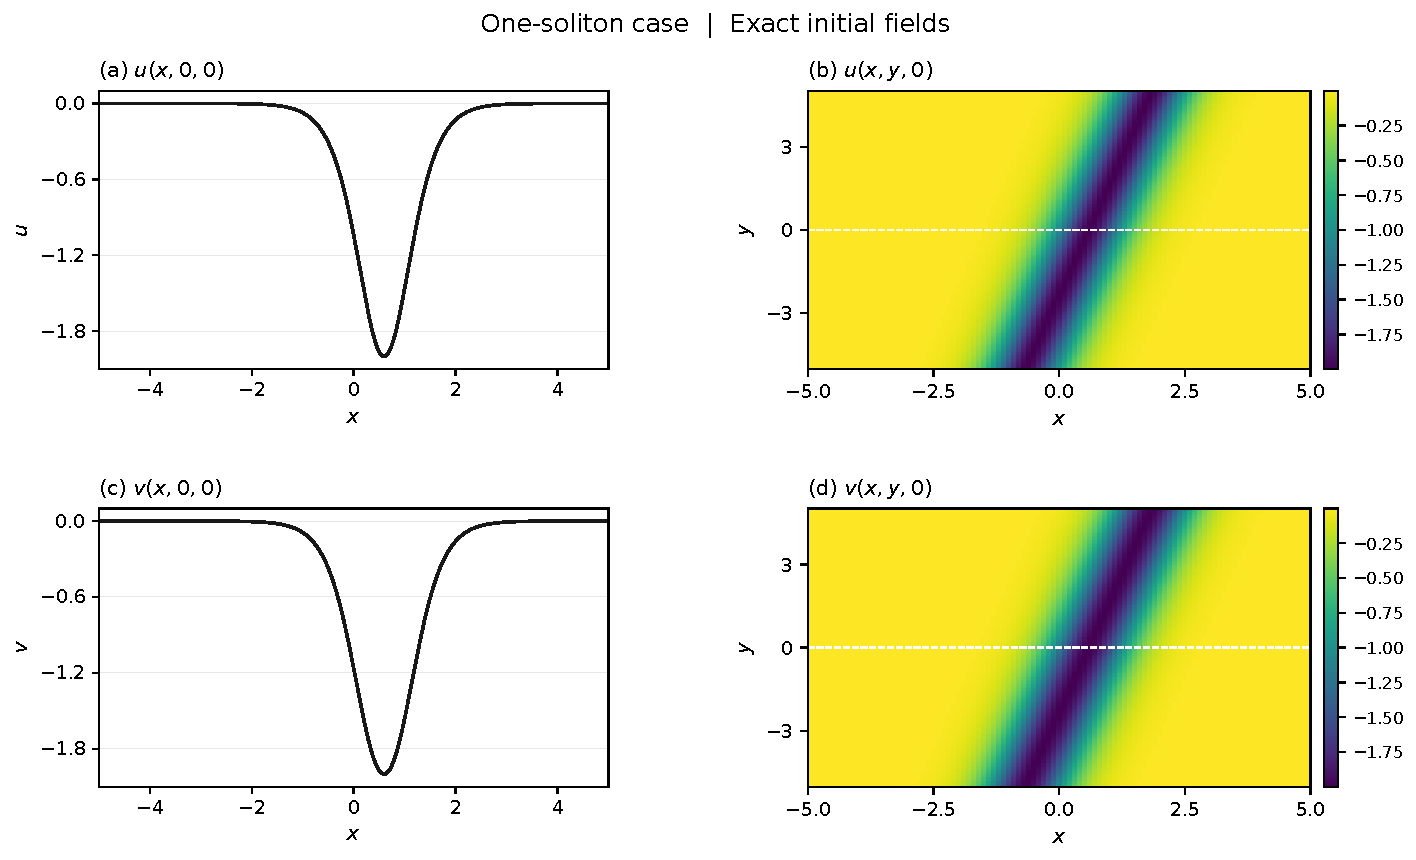
\includegraphics[width=\linewidth,trim=0 196.575bp 0 0,clip]{images/figure-01.pdf}\par
\noindent\begin{minipage}{\linewidth}
\noindent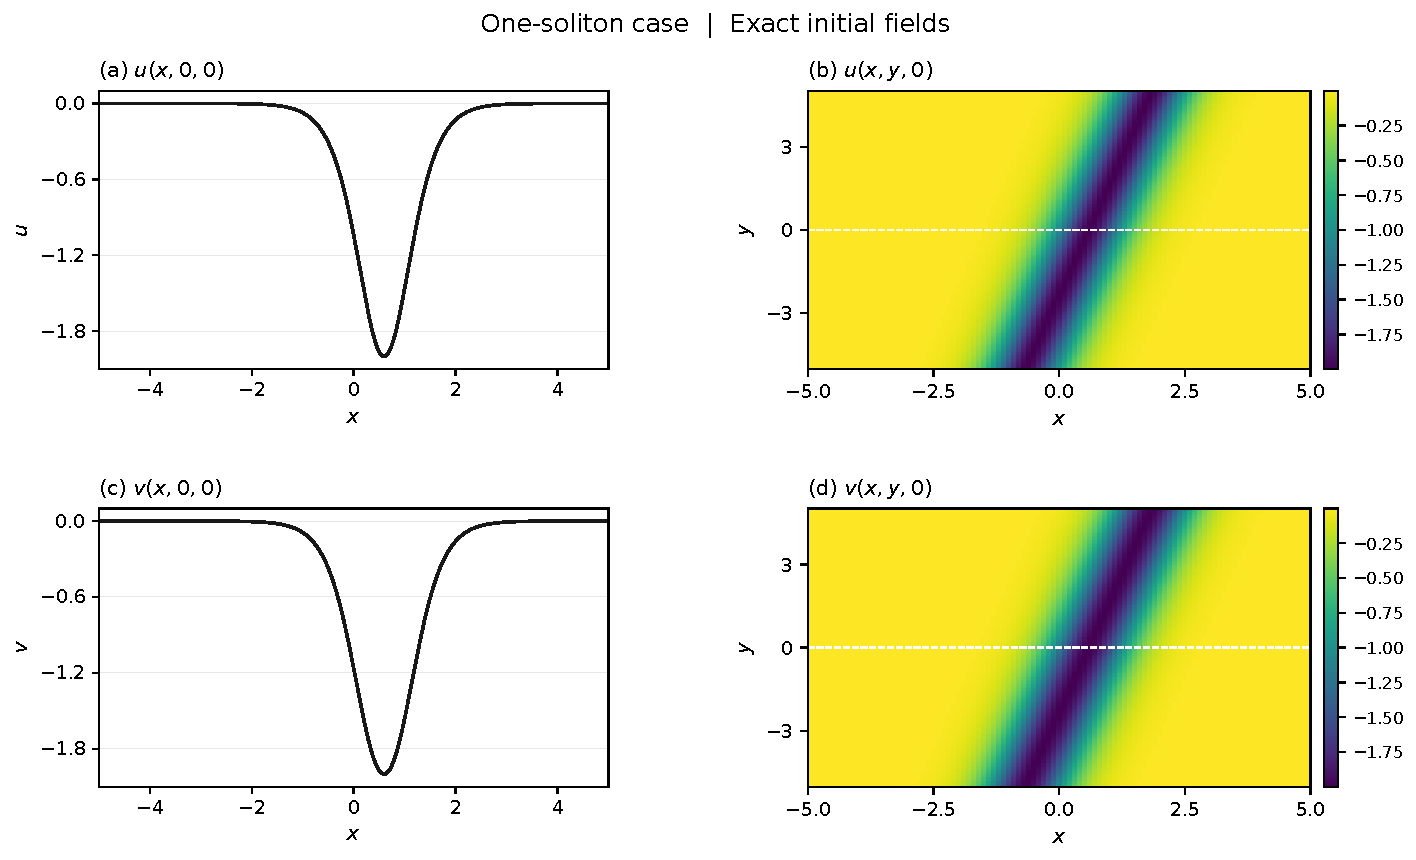
\includegraphics[width=\linewidth,trim=0 0 0 216.000bp,clip]{images/figure-01.pdf}\par
\captionof*{figure}{\textbf{Figure 1.} One-soliton case. Exact initial physical fields. Left: sections at \(y=0\); right: physical-field heatmaps, with the central section marked by a white dashed line. The upper and lower rows show \(u\) and \(v\), respectively.}
\end{minipage}


The two-soliton case (Figure 2) combines the spectral pair of the one-soliton wave with a second pair \((4,-3)\). Its first field \(u\) features a dominant negative trough alongside a shallower positive ridge, whereas both intersecting wave bands remain negative in the second field \(v\), allowing us to test the schemes on interacting waves of different amplitudes and polarities.

\FloatBarrier
\noindent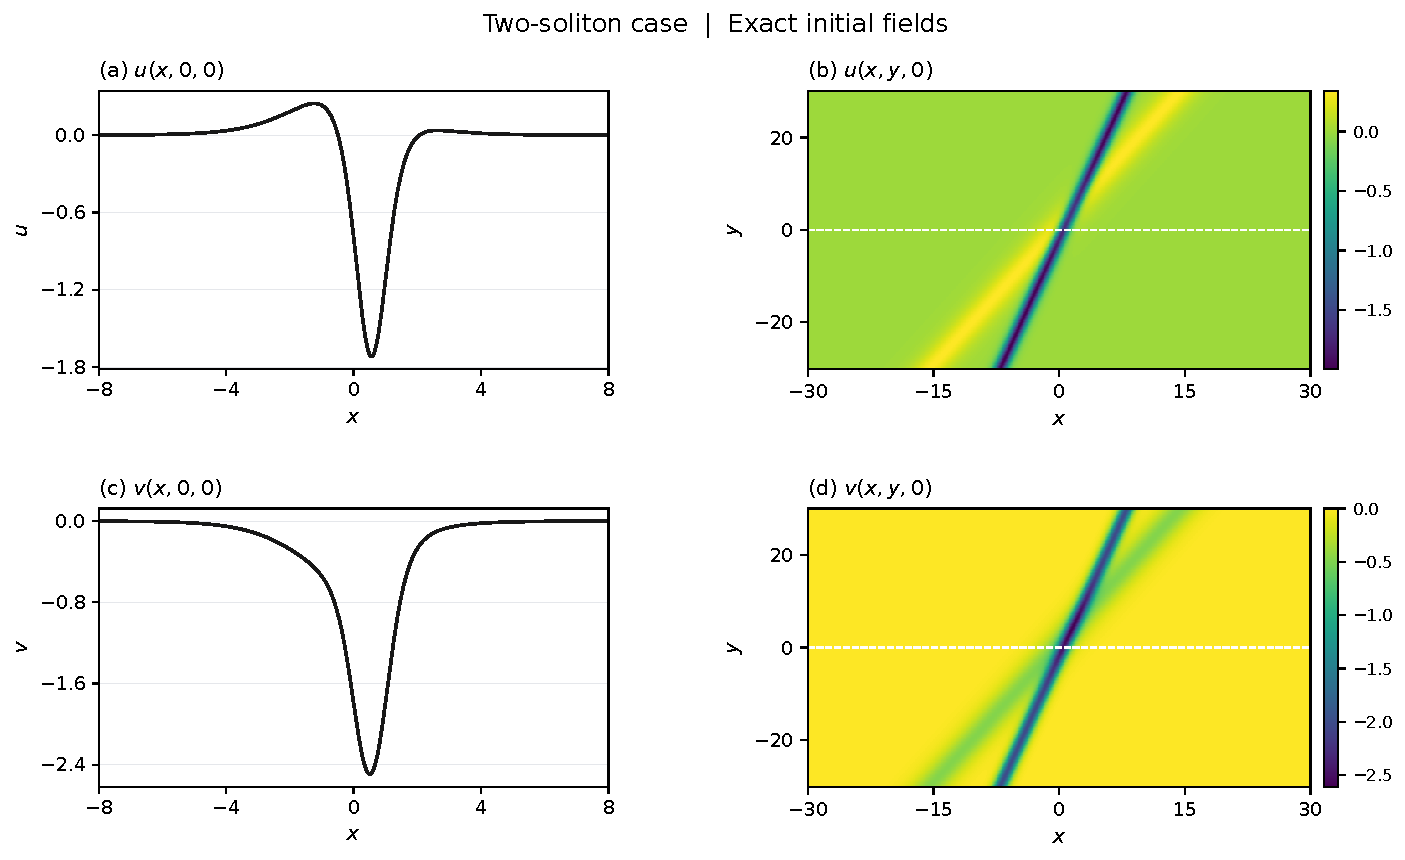
\includegraphics[width=\linewidth,trim=0 196.575bp 0 0,clip]{images/figure-02.pdf}\par
\noindent\begin{minipage}{\linewidth}
\noindent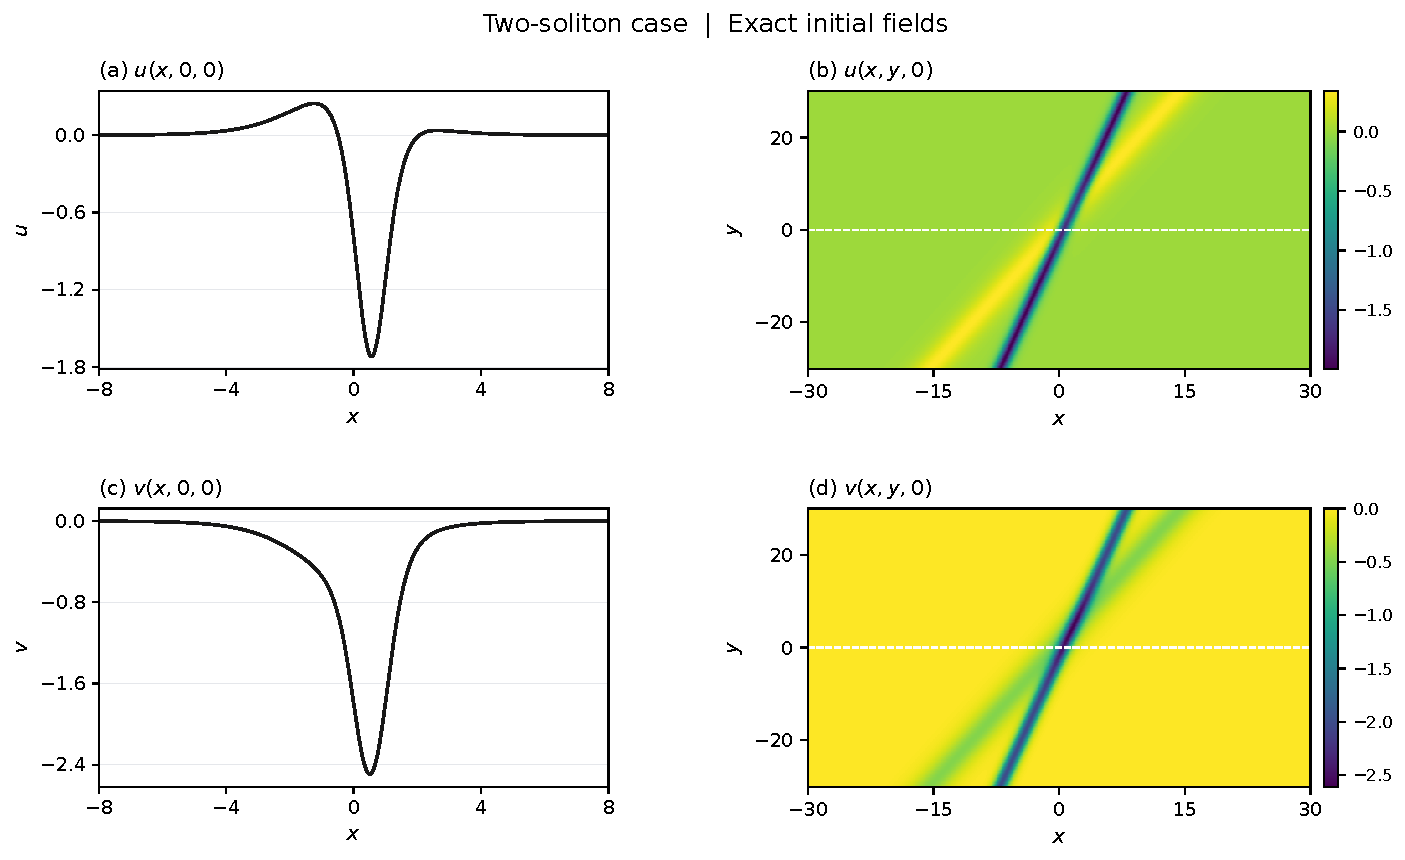
\includegraphics[width=\linewidth,trim=0 0 0 216.000bp,clip]{images/figure-02.pdf}\par
\captionof*{figure}{\textbf{Figure 2.} Two-soliton case. Exact initial physical fields. Left: sections at \(y=0\); right: physical-field heatmaps, with the central section marked by a white dashed line. The upper and lower rows show \(u\) and \(v\), respectively. The section panels focus on \(x\in[-8,8]\); the heatmaps retain the full \([-30,30]\) window.}
\end{minipage}


For the Gaussian and sinusoidal tests, let \(z=y+2\) and \(\kappa=\pi/4\), and take the separable initial fields

\paperdisplay{u_0(x,y)=A\sin(\kappa z)F(x),\qquad v_0(x,y)=4-3A\kappa\cos(\kappa z)F(x).}{\tag{129}}

The Gaussian test uses \(A=0.05\) with the periodic localized profile \(F(x)=\sum_{j\in\mathbb Z}\exp[-((x+192j)/6)^2]\), while the sinusoidal test uses \(A=0.03\) with \(F(x)=\cos(\pi x/12)\). Both problems are computed on the periodic interval \(x\in[-96,96)\) over the transverse strip \(y\in[-2,2]\) with homogeneous lower boundary data \(u=0\).

Because the initial fields satisfy the relation \(v_0=4-3u_{0y}\), the subsequent evolution under the full DLW system can be represented through two linear heat equations and a Laplace transformation over \(0\le t\le0.01\). Interval evaluation of these analytical representations provides continuous reference values and initial time derivatives with an absolute error bound of \(10^{-13}\).

As illustrated in Figure 3, the Gaussian test starts from a localized positive hump in \(u\), while \(v\) varies symmetrically about the background value \(v=4\) with opposite signs in the upper and lower halves of the strip and remains equal to four along the central section \(y=0\).

\FloatBarrier
\noindent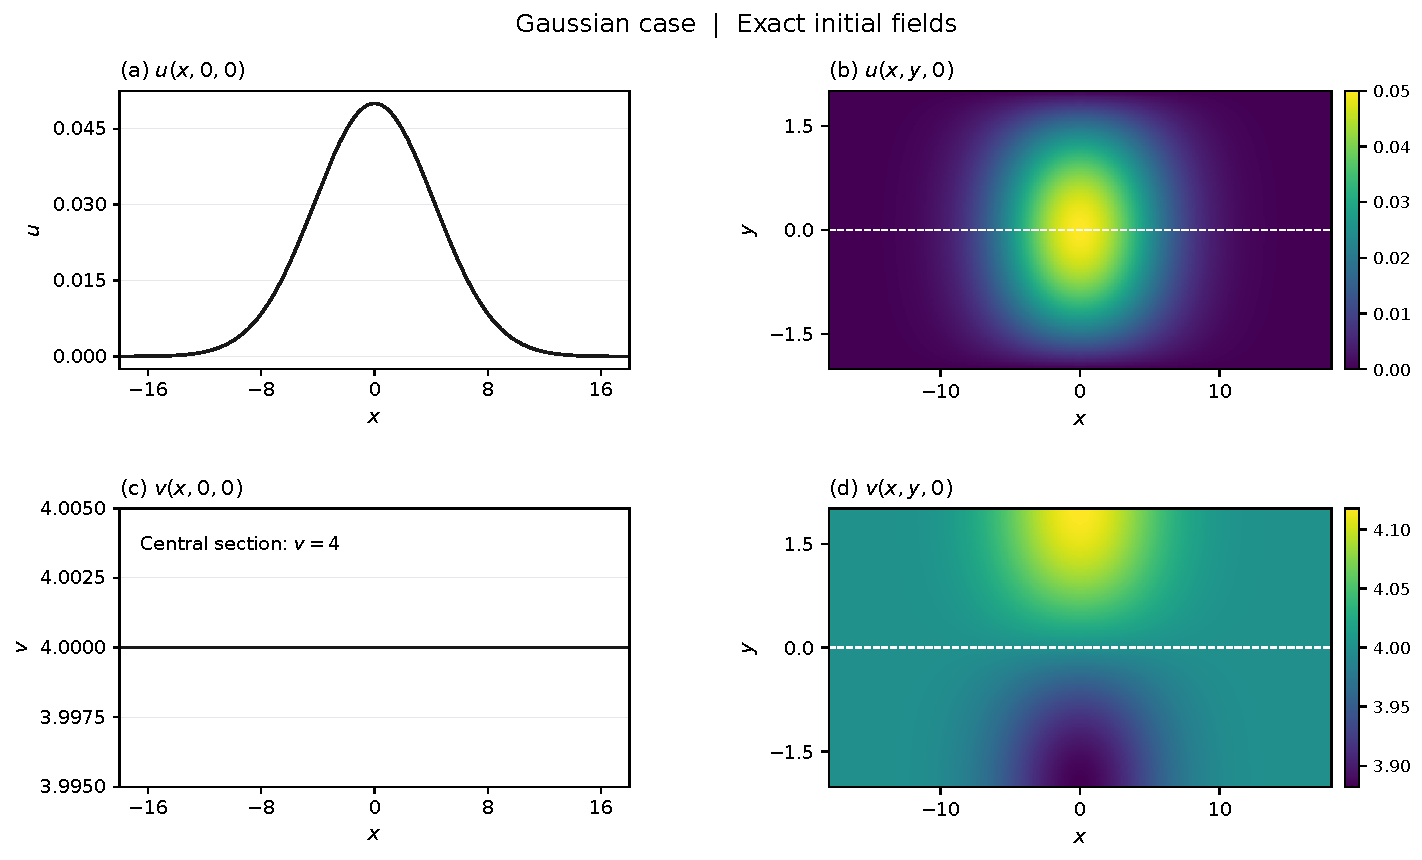
\includegraphics[width=\linewidth,trim=0 196.575bp 0 0,clip]{images/figure-03.pdf}\par
\noindent\begin{minipage}{\linewidth}
\noindent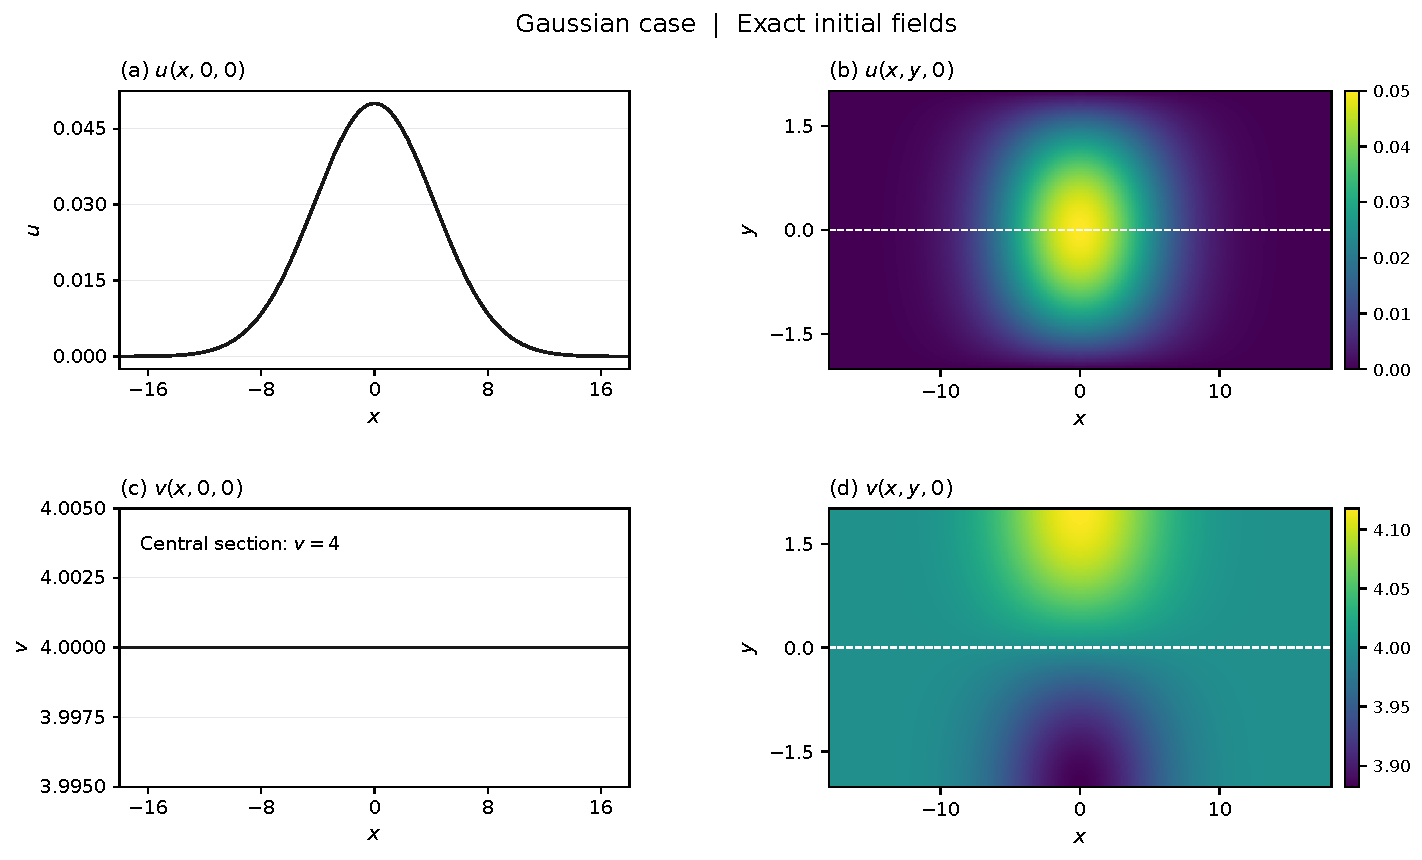
\includegraphics[width=\linewidth,trim=0 0 0 216.000bp,clip]{images/figure-03.pdf}\par
\captionof*{figure}{\textbf{Figure 3.} Gaussian case. Exact initial physical fields. Left: sections at \(y=0\); right: physical-field heatmaps, with the central section marked by a white dashed line. The upper and lower rows show \(u\) and \(v\), respectively. The displayed \(x\) window is \([-18,18]\); the error tables use the full periodic interval \([-96,96)\). The exact central second field satisfies \(v(x,0,t)=4\).}
\end{minipage}


The sinusoidal test (Figure 4) replaces the localized pulse in \(x\) by a periodic cosine wave, so that \(u\) alternates in sign along \(x\) while the departure of \(v\) from its background \(v=4\) reverses sign across \(y=0\).

\FloatBarrier
\noindent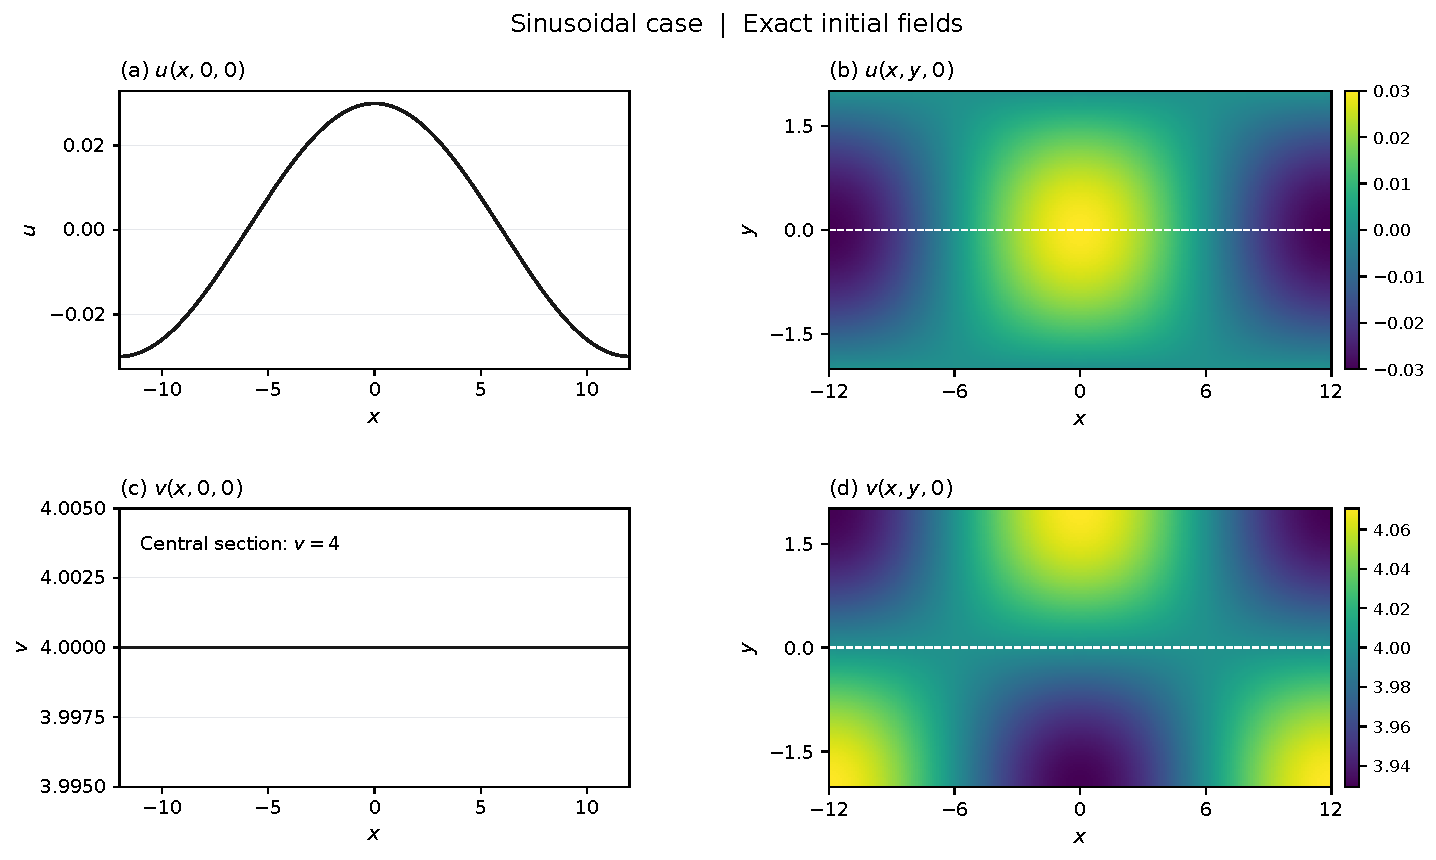
\includegraphics[width=\linewidth,trim=0 196.575bp 0 0,clip]{images/figure-04.pdf}\par
\noindent\begin{minipage}{\linewidth}
\noindent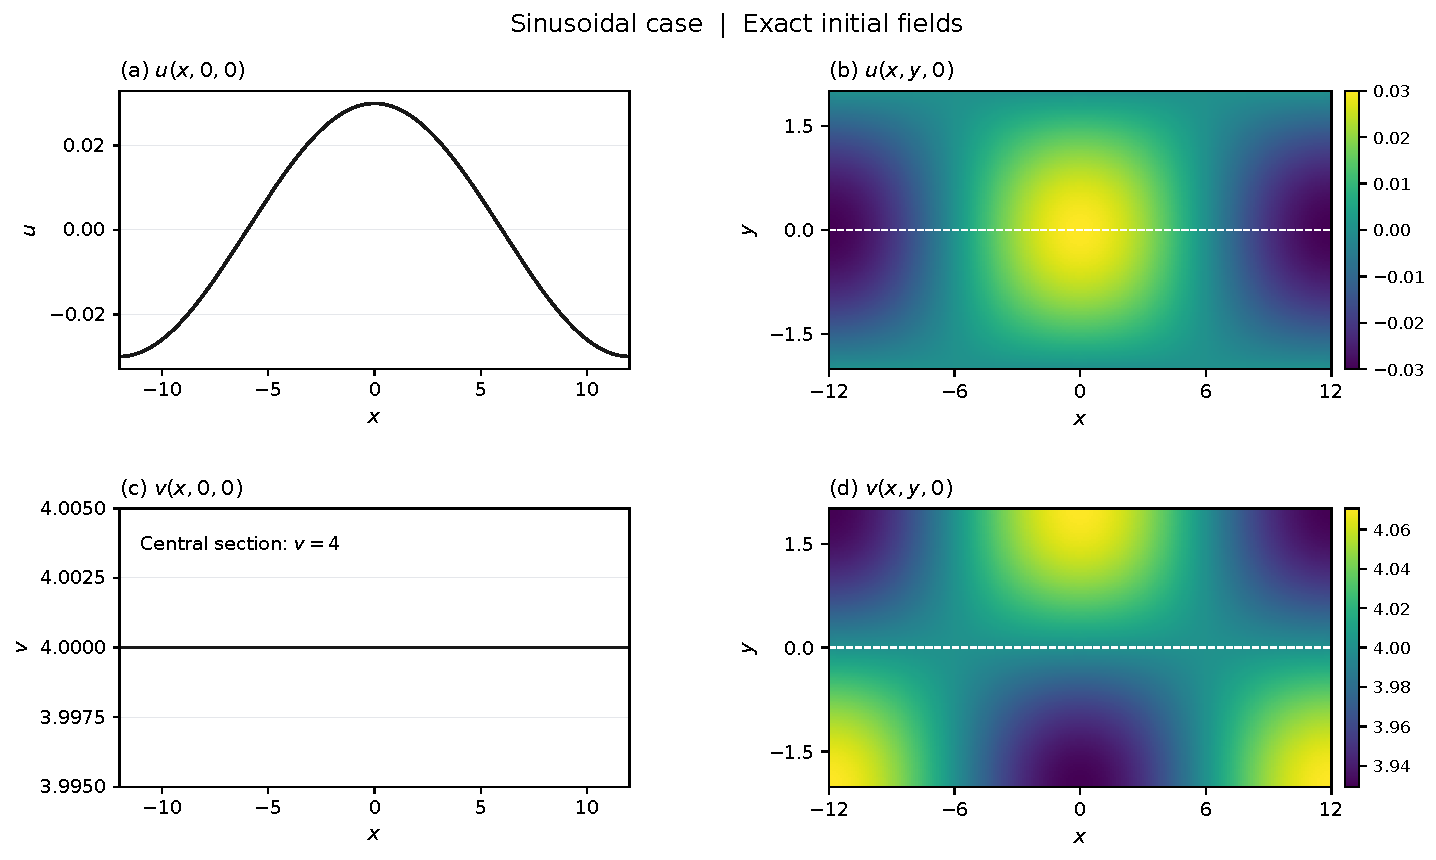
\includegraphics[width=\linewidth,trim=0 0 0 216.000bp,clip]{images/figure-04.pdf}\par
\captionof*{figure}{\textbf{Figure 4.} Sinusoidal case. Exact initial physical fields. Left: sections at \(y=0\); right: physical-field heatmaps, with the central section marked by a white dashed line. The upper and lower rows show \(u\) and \(v\), respectively. The displayed \(x\) window is \([-12,12]\); the error tables use the full periodic interval \([-96,96)\). The exact central second field satisfies \(v(x,0,t)=4\).}
\end{minipage}


Each numerical method is initialized by sampling the continuous reference fields at its native grid locations. Recall that both semi-discrete formulations place \(u\) at transverse nodes and \(v\) at edge midpoints, whereas FD places both fields at the nodes. Errors are evaluated directly at these native sites inside the specified interior region (\(|x|\le R\) and \(|y|<R\) for the soliton tests, and all \(x\) nodes with \(|y|\le1.8\) for the Gaussian and sinusoidal tests). At the final time \(T=0.01\), we record the maximum absolute errors

\paperdisplay{E_u(T)=\max_{\mathcal G_u}\left|u_h(T)-u^*(T)\right|,\qquad E_v(T)=\max_{\mathcal G_v}\left|v_h(T)-v^*(T)\right|,}{\tag{130}}

Here, \(\mathcal G_u\) and \(\mathcal G_v\) denote the native lattice sites of the two physical fields within the evaluation region. We also record the initial derivative errors \(E_{u_t}\) and \(E_{v_t}\), defined as the maximum absolute differences between the spatially computed and exact continuous time derivatives at \(t=0\). These initial errors characterize the spatial approximation before time stepping, while \(E_u(T)\) and \(E_v(T)\) measure the resulting physical-field errors after evolution. Together, they allow us to examine how the initial spatial accuracy is reflected in the computed waves and how the two field components respond during the coupled evolution. In the tables below, bold entries indicate the smallest error among the compared methods for each case and field.

\FloatBarrier
\subsection*{5.2 Comparison of spatial formulations}

In this subsection, we examine how the spatial formulation affects the accuracy of the two physical fields, following the initial spatial approximation through to the computed wave profiles. The analysis in Section 3.4 identifies different truncation errors for Endpoint-SD and Centered-SD, and we use the four test problems to investigate how these differences are reflected in numerical evolution. Direct finite differences applied to the continuous DLW system provide a baseline. All three formulations use \(h=\Delta x=0.1\) and advance from the exact initial data to \(T=0.01\) using classical RK4 with \(\Delta t=10^{-4}\). We first examine the initial time-derivative errors in Table 2, then consider the evolved physical-field errors and their spatial distributions.

\begin{table}[!htbp]
\centering
\caption*{Table 2. Initial time-derivative errors at h = \(\Delta\)x = 0.1.}
\small
\setlength{\tabcolsep}{4pt}
\renewcommand{\arraystretch}{1.22}
\begin{tabularx}{\linewidth}{YYYYYYY}
\toprule
Case & \multicolumn{2}{>{\raggedright\arraybackslash}p{2\dimexpr\linewidth/7-2\tabcolsep\relax}}{Endpoint-SD} & \multicolumn{2}{>{\raggedright\arraybackslash}p{2\dimexpr\linewidth/7-2\tabcolsep\relax}}{Centered-SD} & \multicolumn{2}{>{\raggedright\arraybackslash}p{2\dimexpr\linewidth/7-2\tabcolsep\relax}}{FD} \\
 & \(E_{u_t}\) & \(E_{v_t}\) & \(E_{u_t}\) & \(E_{v_t}\) & \(E_{u_t}\) & \(E_{v_t}\) \\
\midrule
One-soliton & \textbf{2.479 \(\times\) 10\textsuperscript{-3}} & 5.492 \(\times\) 10\textsuperscript{-1} & 1.656 \(\times\) 10\textsuperscript{-2} & \textbf{8.443 \(\times\) 10\textsuperscript{-3}} & 4.957 \(\times\) 10\textsuperscript{-3} & 1.394 \(\times\) 10\textsuperscript{-2} \\
Two-soliton & \textbf{2.142 \(\times\) 10\textsuperscript{-3}} & 7.010 \(\times\) 10\textsuperscript{-1} & 1.295 \(\times\) 10\textsuperscript{-2} & \textbf{1.089 \(\times\) 10\textsuperscript{-2}} & 4.284 \(\times\) 10\textsuperscript{-3} & 1.644 \(\times\) 10\textsuperscript{-2} \\
Gaussian & \textbf{2.142 \(\times\) 10\textsuperscript{-6}} & 6.038 \(\times\) 10\textsuperscript{-5} & 2.900 \(\times\) 10\textsuperscript{-6} & \textbf{6.997 \(\times\) 10\textsuperscript{-7}} & 4.284 \(\times\) 10\textsuperscript{-6} & 2.215 \(\times\) 10\textsuperscript{-6} \\
Sinusoidal & \textbf{1.586 \(\times\) 10\textsuperscript{-6}} & 2.833 \(\times\) 10\textsuperscript{-5} & 2.003 \(\times\) 10\textsuperscript{-6} & \textbf{4.715 \(\times\) 10\textsuperscript{-7}} & 3.171 \(\times\) 10\textsuperscript{-6} & 1.639 \(\times\) 10\textsuperscript{-6} \\
\bottomrule
\end{tabularx}
\end{table}

At \(t=0\), the two semi-discrete formulations show a clear division between the two components: Endpoint-SD gives the smallest initial \(u_t\) defect \(E_{u_t}\) in all four cases, whereas Centered-SD gives the smallest \(v_t\) defect \(E_{v_t}\). This pattern is consistent with Proposition 3.4. In the first equation, both formulations are second-order consistent, and the difference in \(E_{u_t}\) comes from the \(O(h^2)\) auxiliary flux term retained by Centered-SD. In the second equation, however, the one-sided pairing of Endpoint-SD leaves a first-order \(O(h)\) truncation term, which makes its initial \(v_t\) error significantly larger than those of Centered-SD and FD.

Table 3 follows these initial states to \(T=0.01\) and reports the resulting errors in the physical fields \(u\) and \(v\). In the accompanying figures, the cross-section panels compare the continuous reference profiles at \(y=0\) with the numerical values (using a verified 12-point local polynomial interpolation in \(y\) whenever \(y=0\) lies between native lattice lines), while the heatmaps display the spatial distribution of the absolute errors across the evaluation region.

\begin{table}[!htbp]
\centering
\caption*{Table 3. Physical-field errors at T = 0.01 with RK4, \(\Delta\)t = 10\textsuperscript{-}\textsuperscript{4} and h = \(\Delta\)x = 0.1.}
\small
\setlength{\tabcolsep}{4pt}
\renewcommand{\arraystretch}{1.22}
\begin{tabularx}{\linewidth}{YYYYYYY}
\toprule
Case & \multicolumn{2}{>{\raggedright\arraybackslash}p{2\dimexpr\linewidth/7-2\tabcolsep\relax}}{Endpoint-SD} & \multicolumn{2}{>{\raggedright\arraybackslash}p{2\dimexpr\linewidth/7-2\tabcolsep\relax}}{Centered-SD} & \multicolumn{2}{>{\raggedright\arraybackslash}p{2\dimexpr\linewidth/7-2\tabcolsep\relax}}{FD} \\
 & \(E_u\) & \(E_v\) & \(E_u\) & \(E_v\) & \(E_u\) & \(E_v\) \\
\midrule
One-soliton & 4.702 \(\times\) 10\textsuperscript{-4} & 5.547 \(\times\) 10\textsuperscript{-3} & 1.677 \(\times\) 10\textsuperscript{-4} & \textbf{7.734 \(\times\) 10\textsuperscript{-5}} & \textbf{5.568 \(\times\) 10\textsuperscript{-5}} & 1.428 \(\times\) 10\textsuperscript{-4} \\
Two-soliton & 4.942 \(\times\) 10\textsuperscript{-4} & 7.076 \(\times\) 10\textsuperscript{-3} & 1.792 \(\times\) 10\textsuperscript{-4} & \textbf{1.009 \(\times\) 10\textsuperscript{-4}} & \textbf{1.149 \(\times\) 10\textsuperscript{-4}} & 1.694 \(\times\) 10\textsuperscript{-4} \\
Gaussian & \textbf{2.147 \(\times\) 10\textsuperscript{-8}} & 6.036 \(\times\) 10\textsuperscript{-7} & 2.900 \(\times\) 10\textsuperscript{-8} & \textbf{6.967 \(\times\) 10\textsuperscript{-9}} & 4.280 \(\times\) 10\textsuperscript{-8} & 2.206 \(\times\) 10\textsuperscript{-8} \\
Sinusoidal & \textbf{1.588 \(\times\) 10\textsuperscript{-8}} & 2.833 \(\times\) 10\textsuperscript{-7} & 2.003 \(\times\) 10\textsuperscript{-8} & \textbf{4.706 \(\times\) 10\textsuperscript{-9}} & 3.170 \(\times\) 10\textsuperscript{-8} & 1.637 \(\times\) 10\textsuperscript{-8} \\
\bottomrule
\end{tabularx}
\end{table}

Looking across Table 3, we see that Centered-SD maintains the smallest \(v\) error in all four tests, while the ordering of the \(u\) error depends on the test problem.

\subsubsection*{One-soliton and two-soliton cases}

Figure 5(a,c) shows the one-soliton profiles along \(y=0\). Both fields form a localized depression, with a single trough and a return toward the background on either side. The numerical symbols from all three formulations follow the continuous reference closely, resolving both the trough and its flanks. Panels (b,d) make their differences visible through the absolute errors along the same section. These errors have several local peaks around the wave, with a particularly clear separation between Endpoint-SD and the other two methods in \(v\).

Comparing the two semi-discrete schemes, we notice that Centered-SD not only reduces the terminal \(v\) error relative to Endpoint-SD by a factor of \(72\) (from \(5.547\times10^{-3}\) to \(7.734\times10^{-5}\)), but also achieves a smaller terminal \(u\) error by a factor of \(2.8\) (reducing \(E_u\) from \(4.702\times10^{-4}\) to \(1.677\times10^{-4}\)), reversing their initial ordering in Table 2. A simple explanation for this reversal lies in the coupled evolution of the two fields: because the first DLW equation contains the dispersive term \(v_{xx}\), the much larger \(O(h)\) error incurred by Endpoint-SD in \(v\) feeds back into the time derivative of \(u\) as the wave evolves, whereas the symmetric staggered arrangement of Centered-SD keeps both components at second order.

The heatmaps in Figure 5(e–j) extend this section comparison to the two-dimensional region. The dashed horizontal line marks \(y=0\), linking the upper panels to the maps below. Bands of larger error follow the inclined wave structure, with narrow low-error strips separating local maxima. The common color scale within each field makes the smaller \(v\) errors of Centered-SD and FD visible alongside the broader, brighter Endpoint-SD error band.

\FloatBarrier
\noindent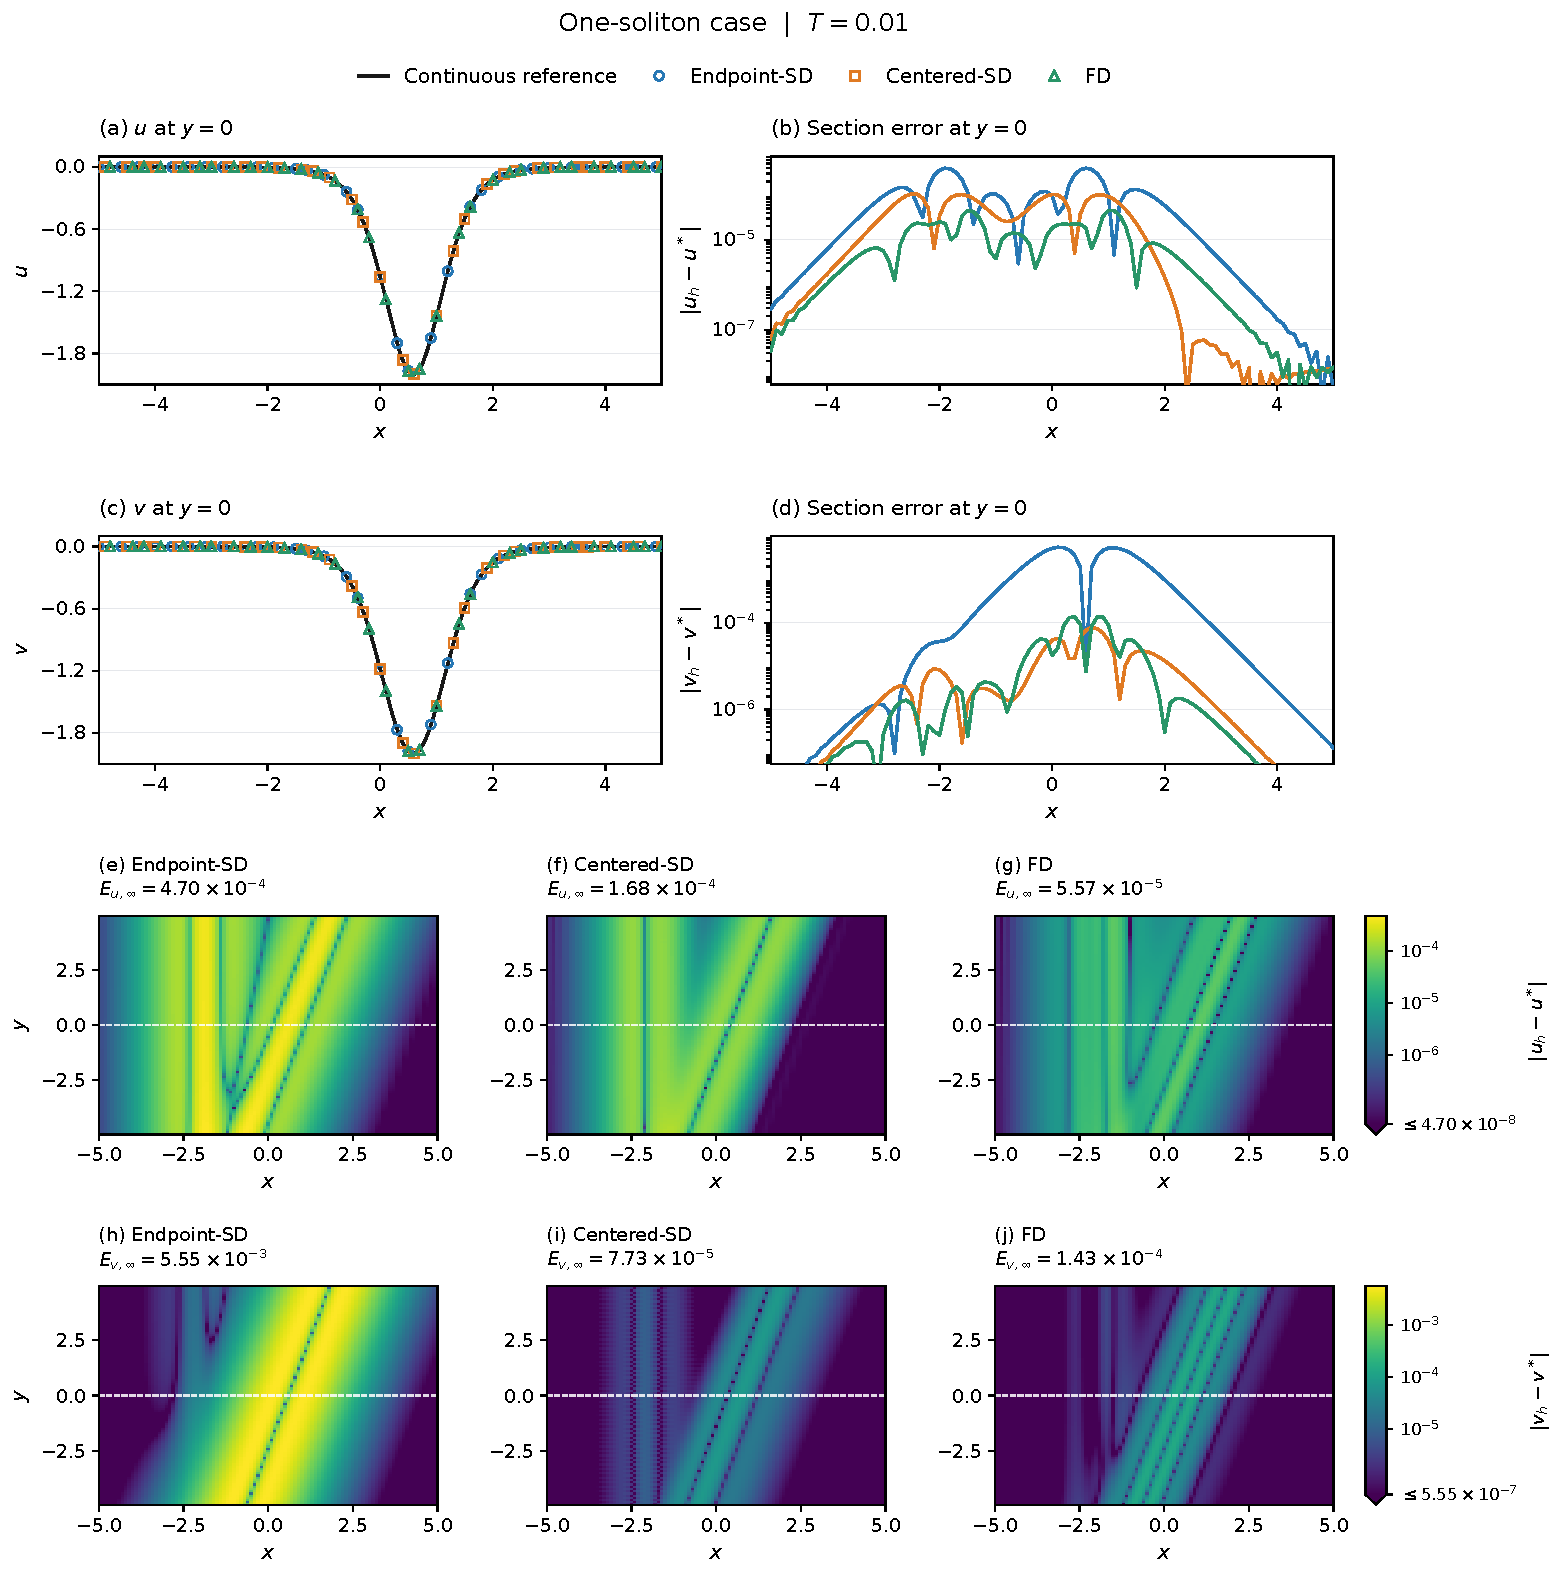
\includegraphics[width=\linewidth,trim=0 532.383bp 0 0.000bp,clip]{images/figure-05.pdf}\par
\noindent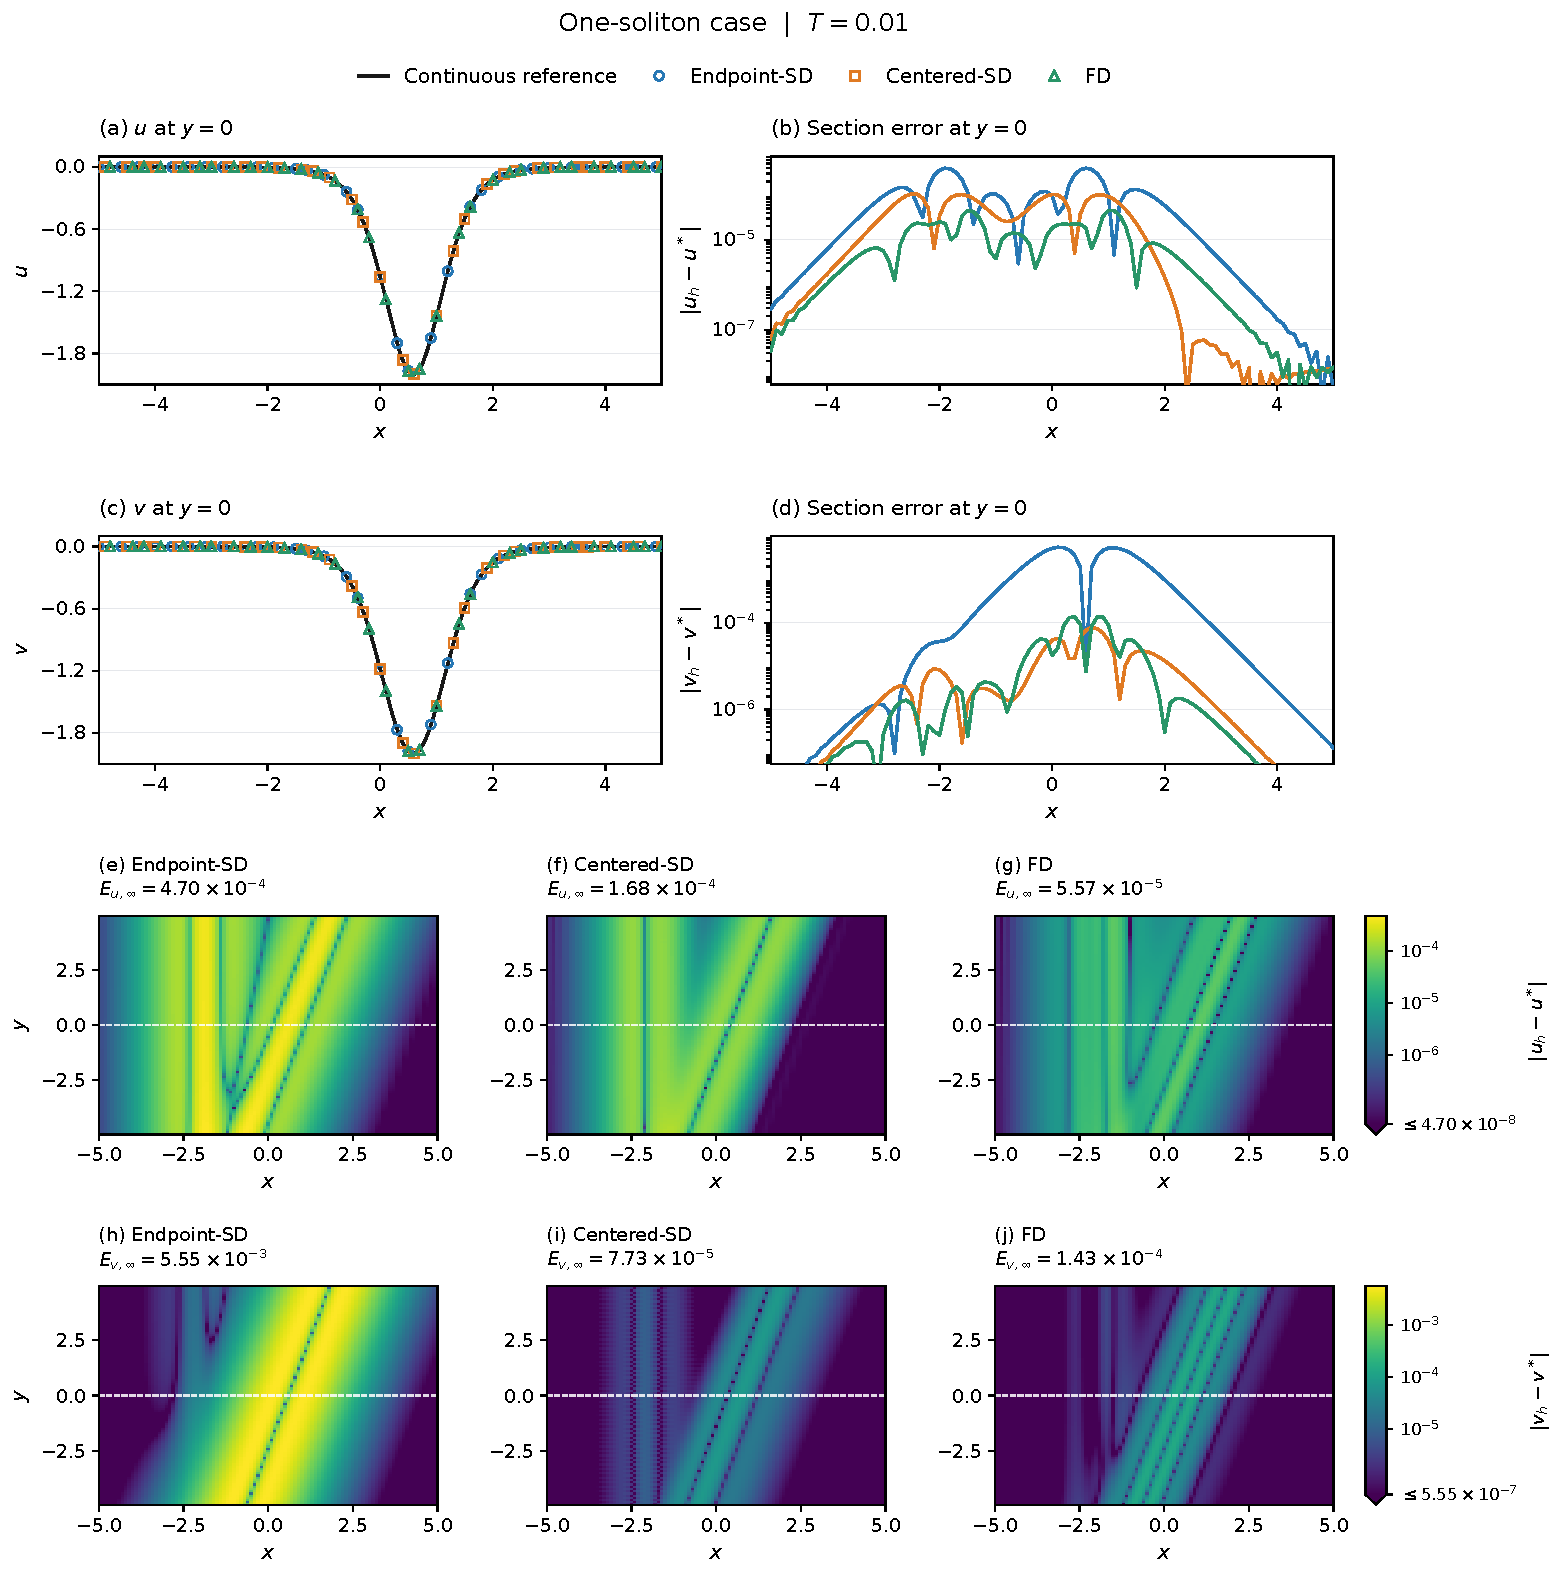
\includegraphics[width=\linewidth,trim=0 355.883bp 0 224.000bp,clip]{images/figure-05.pdf}\par
\noindent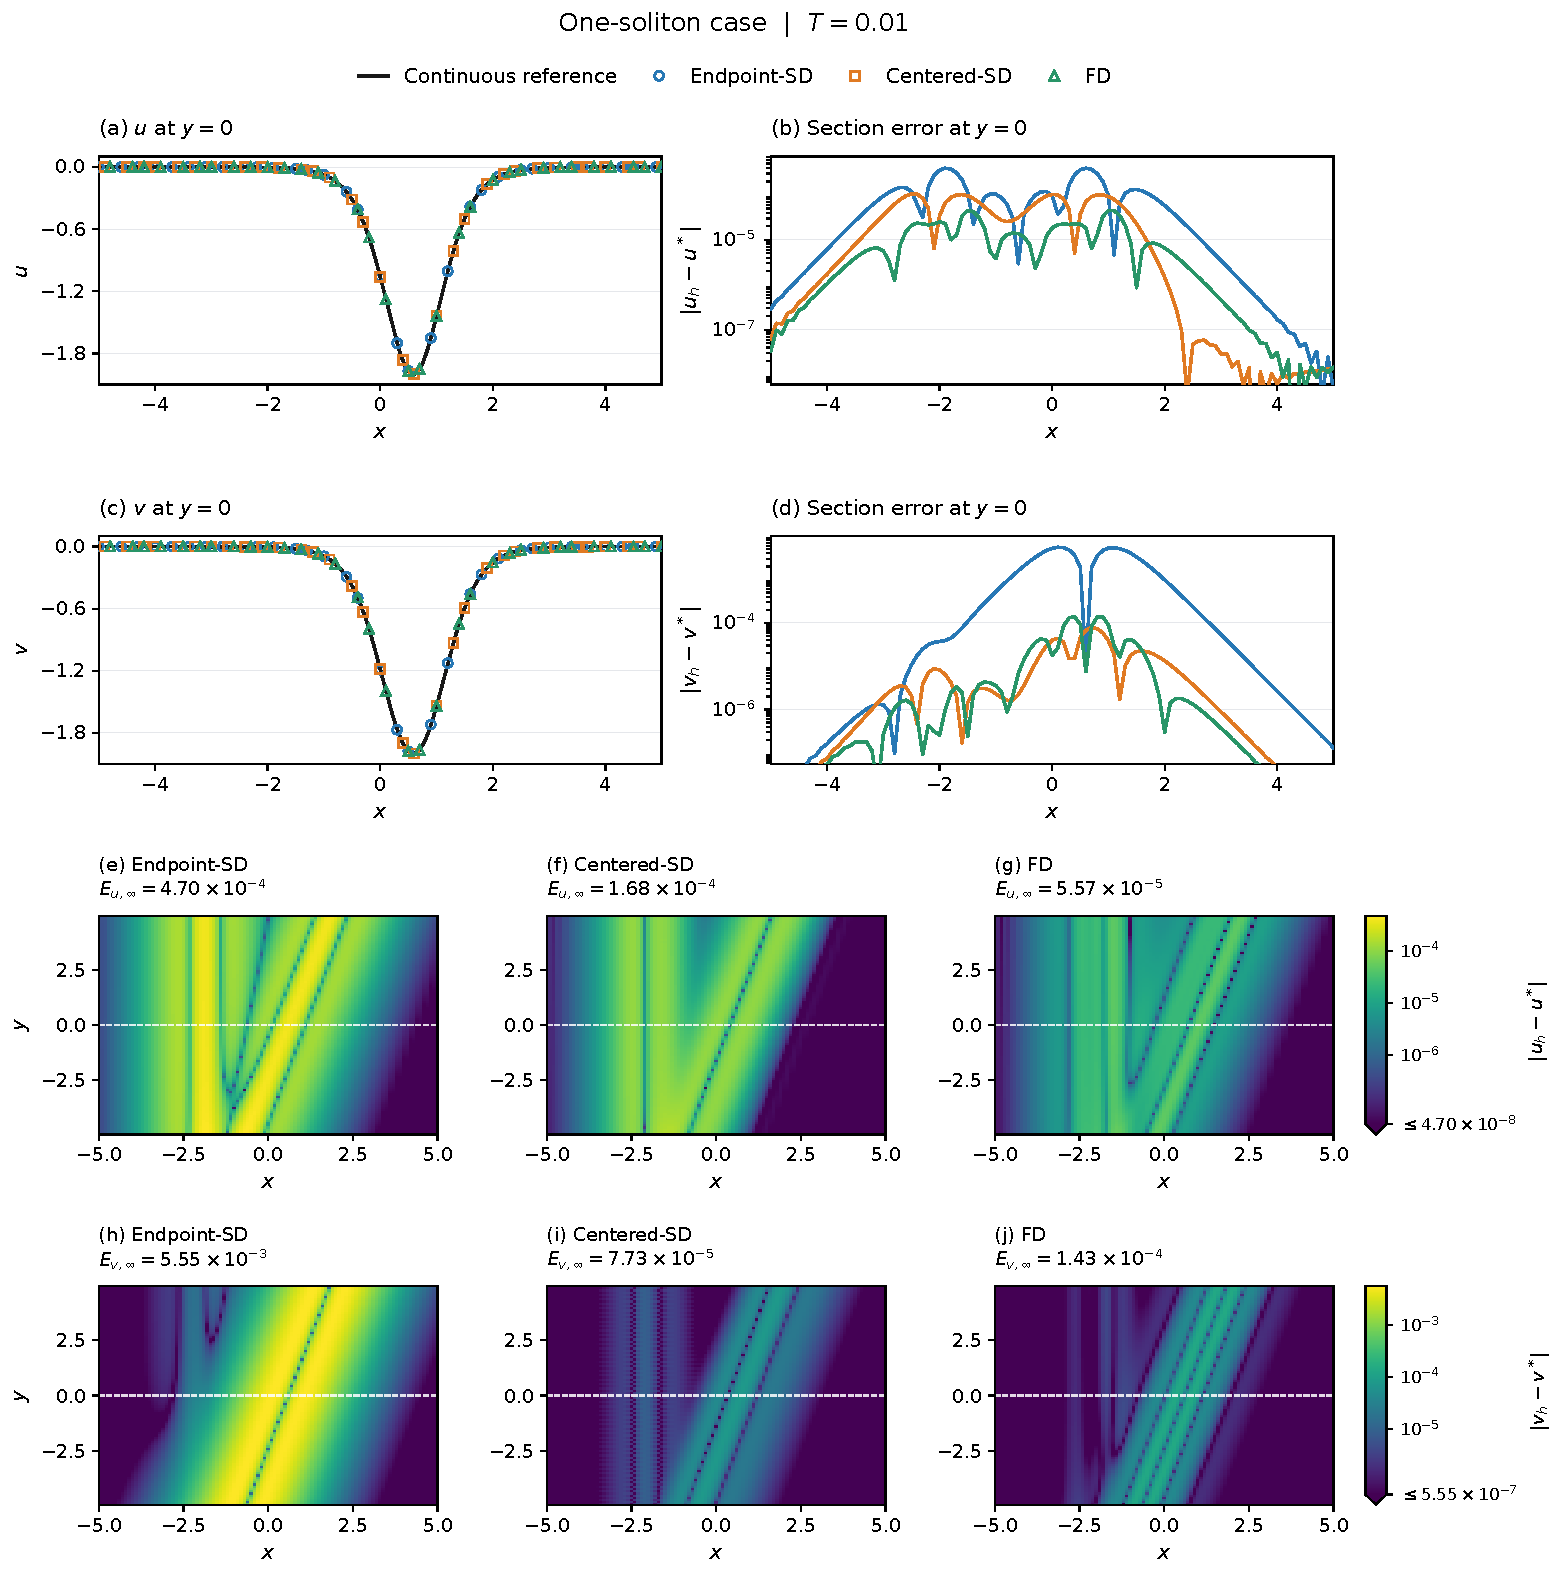
\includegraphics[width=\linewidth,trim=0 177.383bp 0 400.500bp,clip]{images/figure-05.pdf}\par
\noindent\begin{minipage}{\linewidth}
\noindent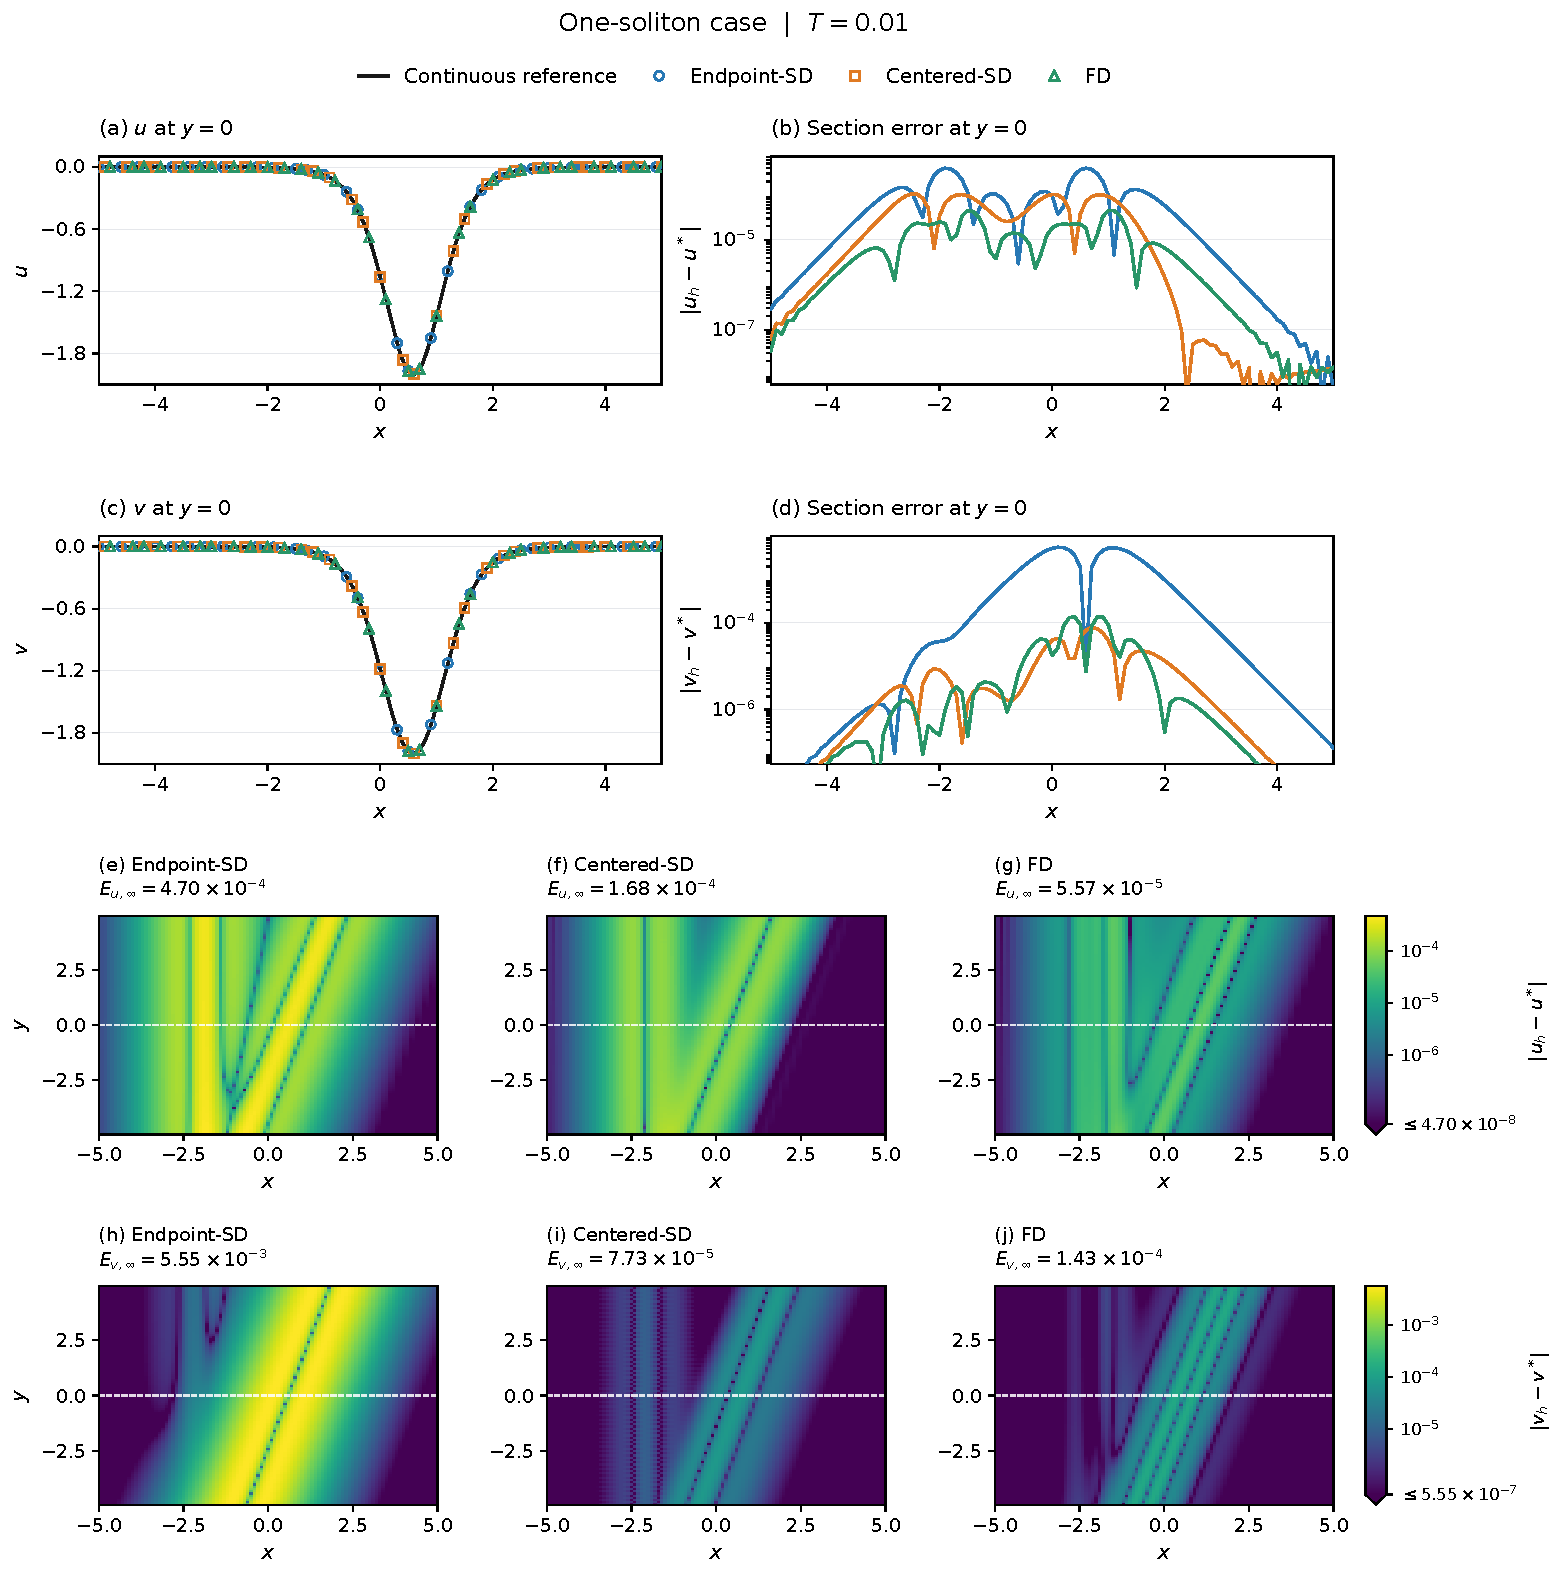
\includegraphics[width=\linewidth,trim=0 0.000bp 0 579.000bp,clip]{images/figure-05.pdf}\par
\captionof*{figure}{\textbf{Figure 5.} One-soliton case at \(T=0.01\). Panels (a,c) compare the continuous \(y=0\) profiles with numerical symbols; panels (b,d) show the absolute errors along that section. The lower rows show the \(u\) and \(v\) error maps, with columns for Endpoint-SD, Centered-SD and FD. Each row uses one logarithmic color scale; values at or below its lower limit, including zero, share the darkest color, as indicated by the \(\leq\) label on the colorbar. Panel maxima refer to the full table region.}
\end{minipage}





The two-soliton section in Figure 6(a,c) has a more asymmetric shape. Along \(y=0\), the \(u\) profile has a small positive shoulder to the left of a pronounced negative trough, while \(v\) has a broader depression leading into a deeper minimum. The numerical values reproduce these features closely. The section errors in panels (b,d) resolve the differences beneath this visual agreement, including local oscillations and larger errors near the central trough.

Relative to Endpoint-SD, Centered-SD reduces the terminal \(u\) error from \(4.942\times10^{-4}\) to \(1.792\times10^{-4}\) and the \(v\) error from \(7.076\times10^{-3}\) to \(1.009\times10^{-4}\). The improvement factors — about \(2.8\) in \(u\) and \(70\) in \(v\) — are nearly identical to those observed in the single-soliton case, and Centered-SD also improves upon the FD baseline in the second field by a factor of about \(1.7\).

The heatmaps in Figure 6(e–j) show how this error pattern extends across the two-dimensional wave configuration. Several bands and their intersections are visible over the wider plotting region, whereas the upper panels focus on the central section. In \(v\), the dominant oblique band is substantially brighter for Endpoint-SD; the Centered-SD and FD maps retain a narrower band of larger error. These maps locate the errors reported in Table 3 and show their variation away from \(y=0\).

\FloatBarrier
\noindent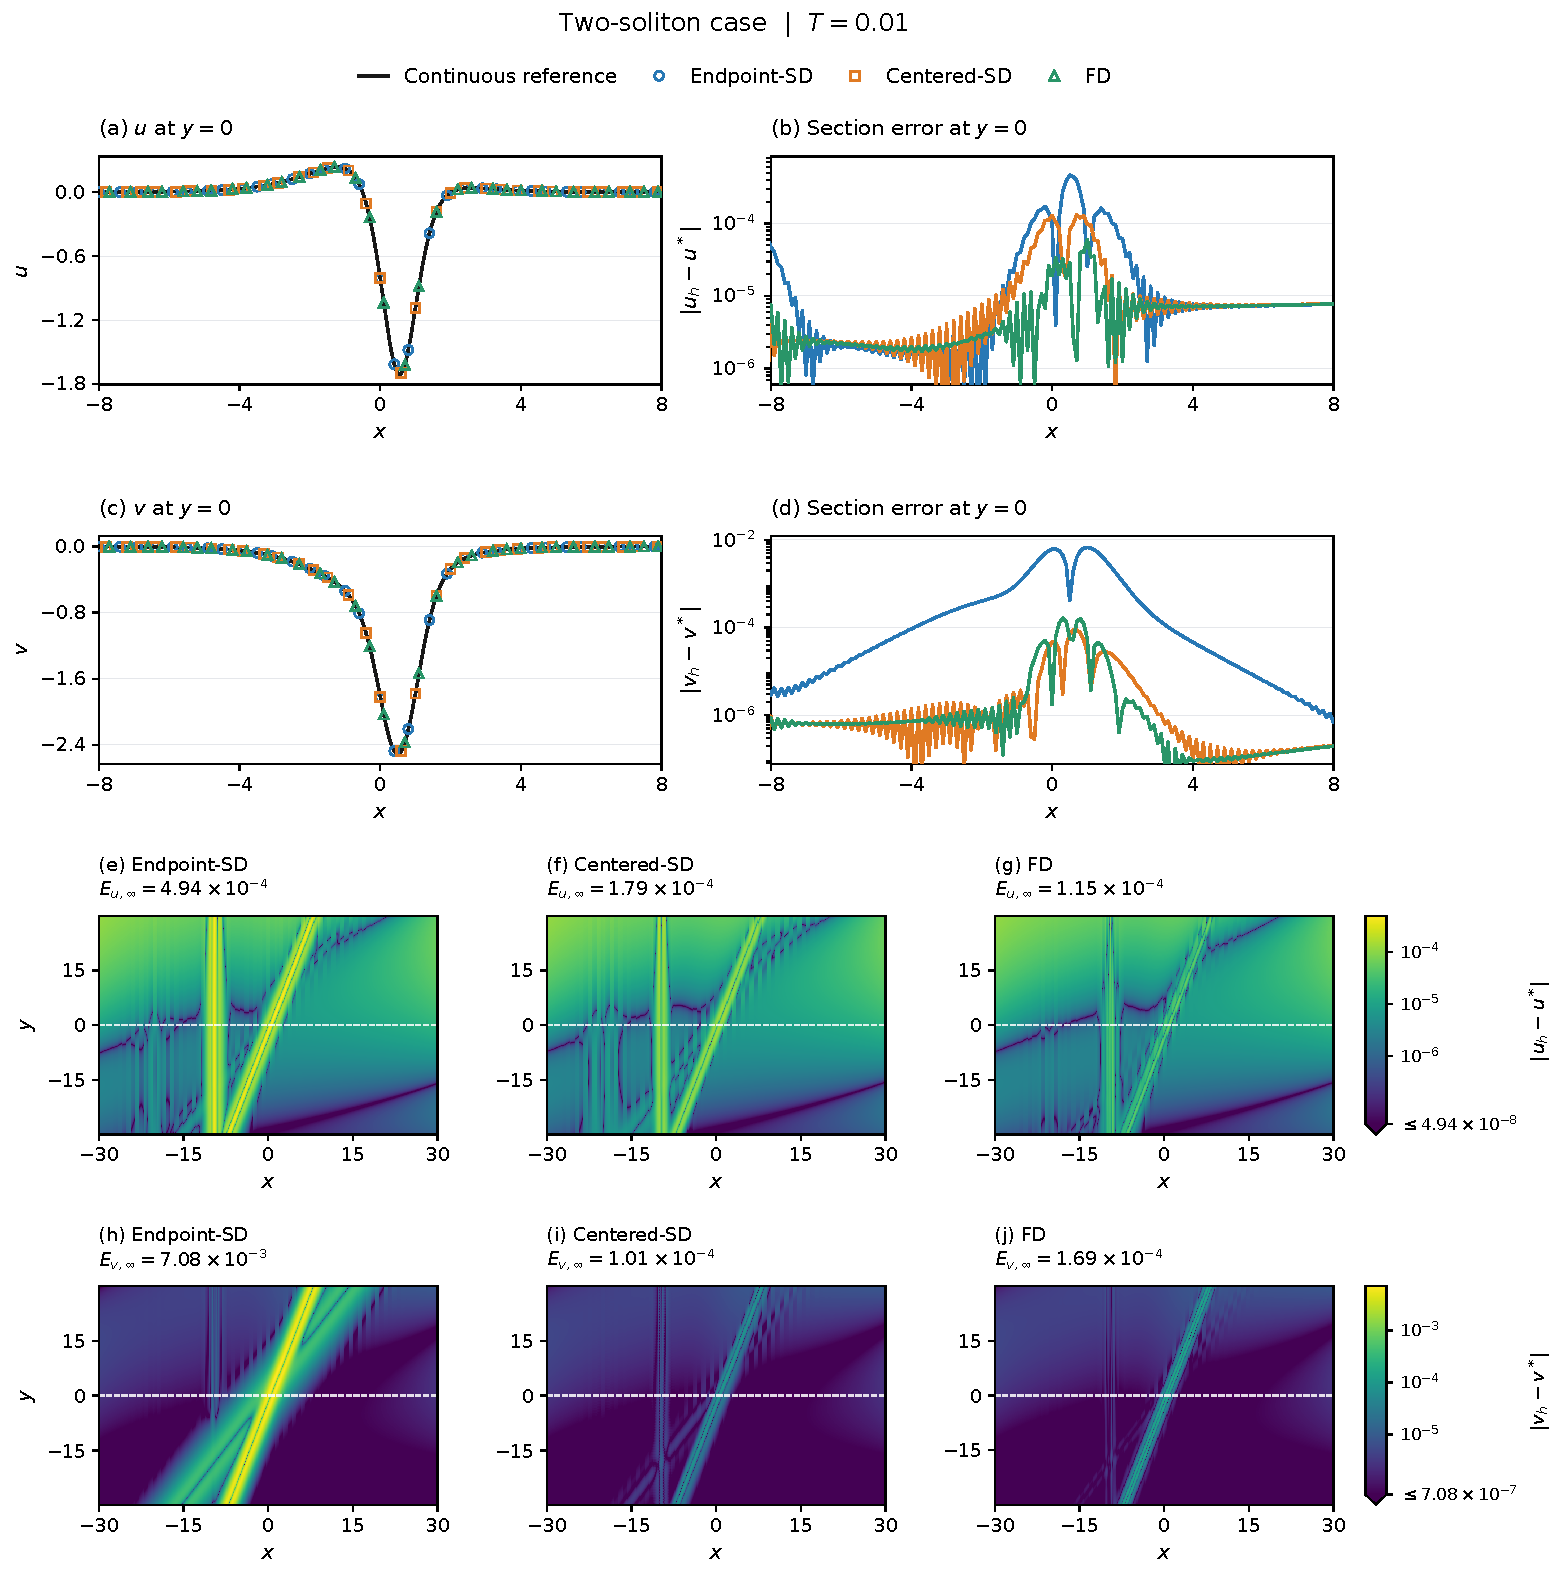
\includegraphics[width=\linewidth,trim=0 532.383bp 0 0.000bp,clip]{images/figure-06.pdf}\par
\noindent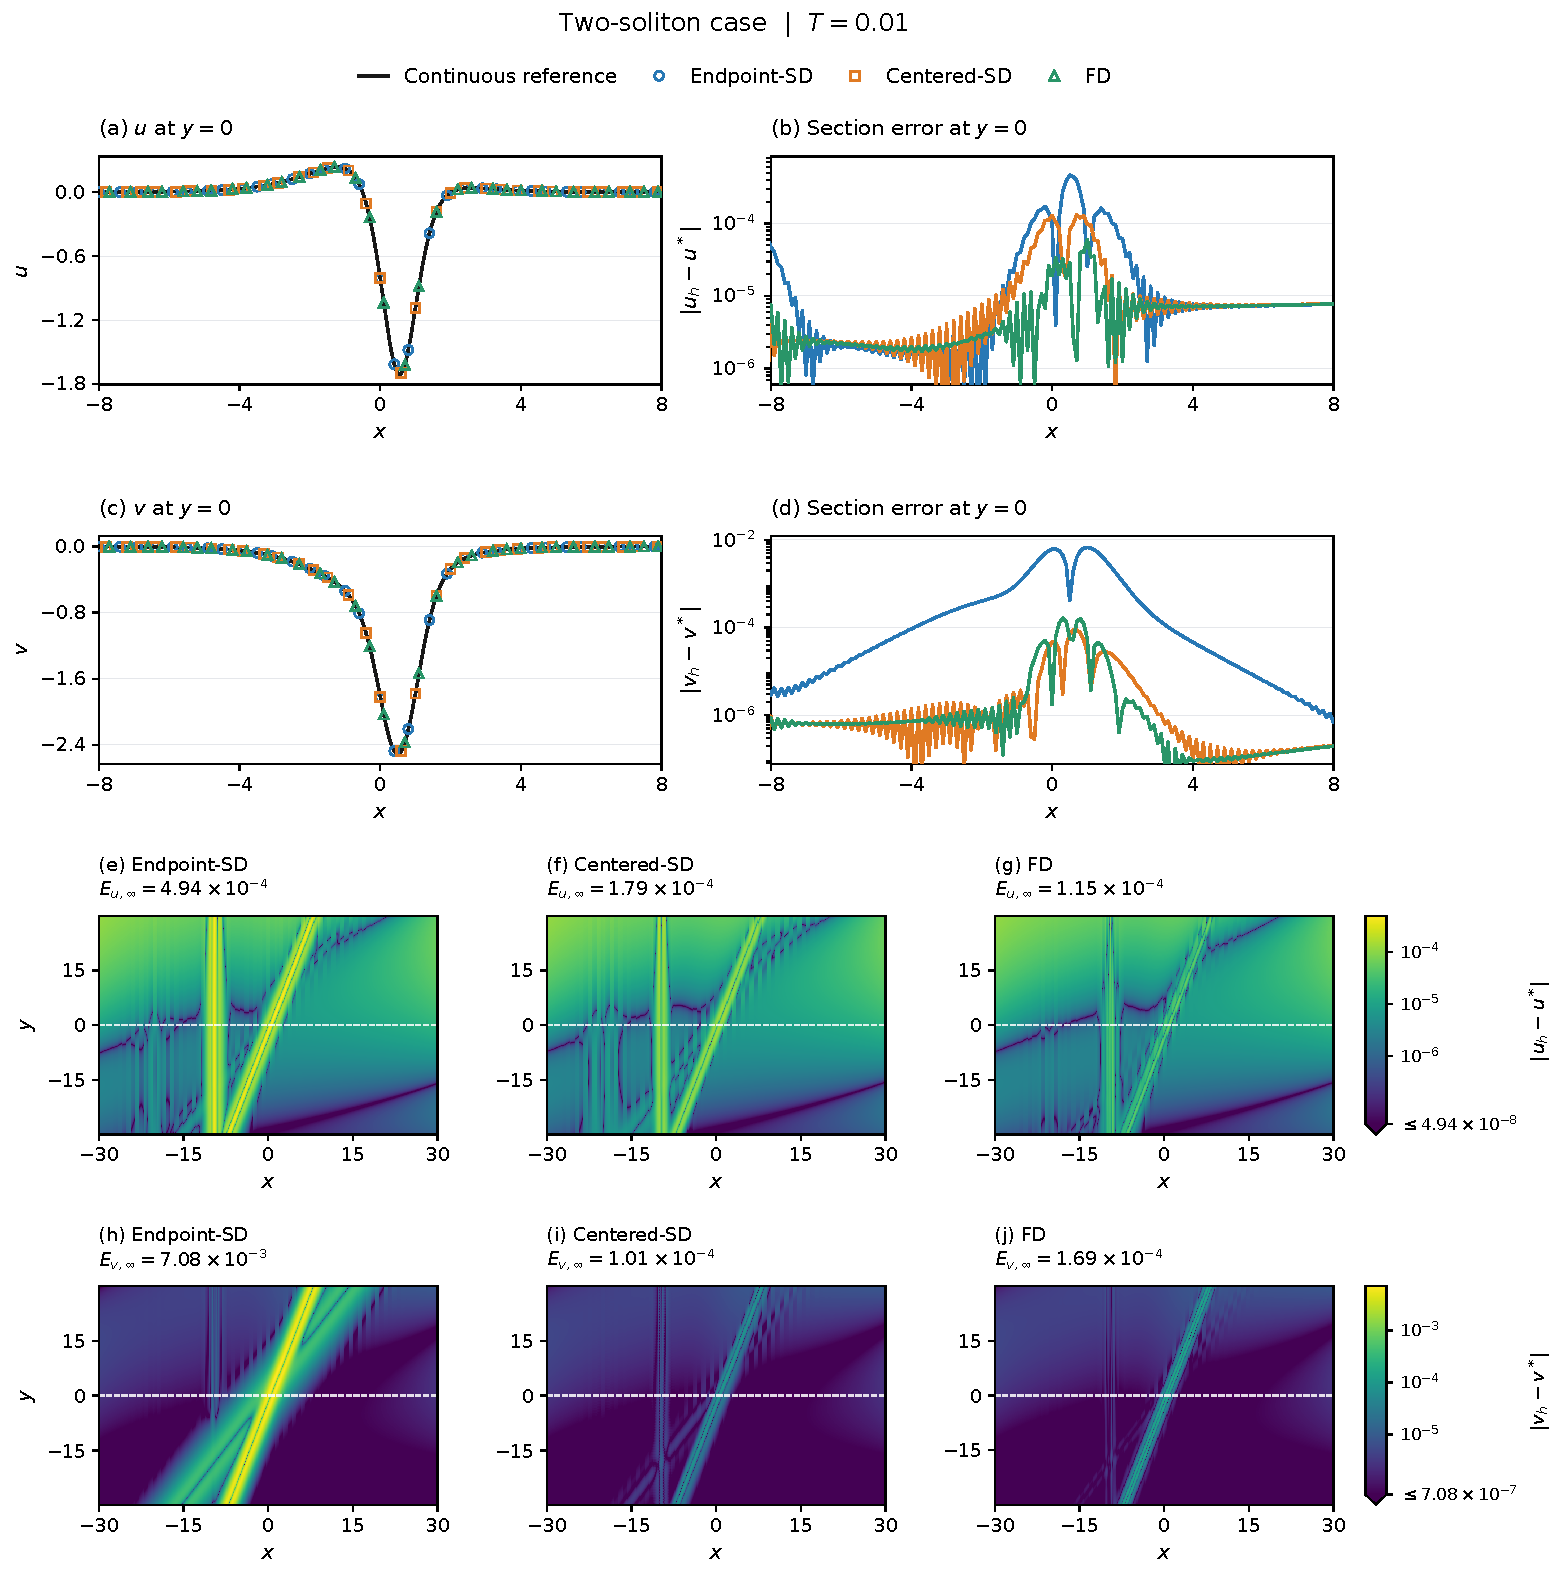
\includegraphics[width=\linewidth,trim=0 355.883bp 0 224.000bp,clip]{images/figure-06.pdf}\par
\noindent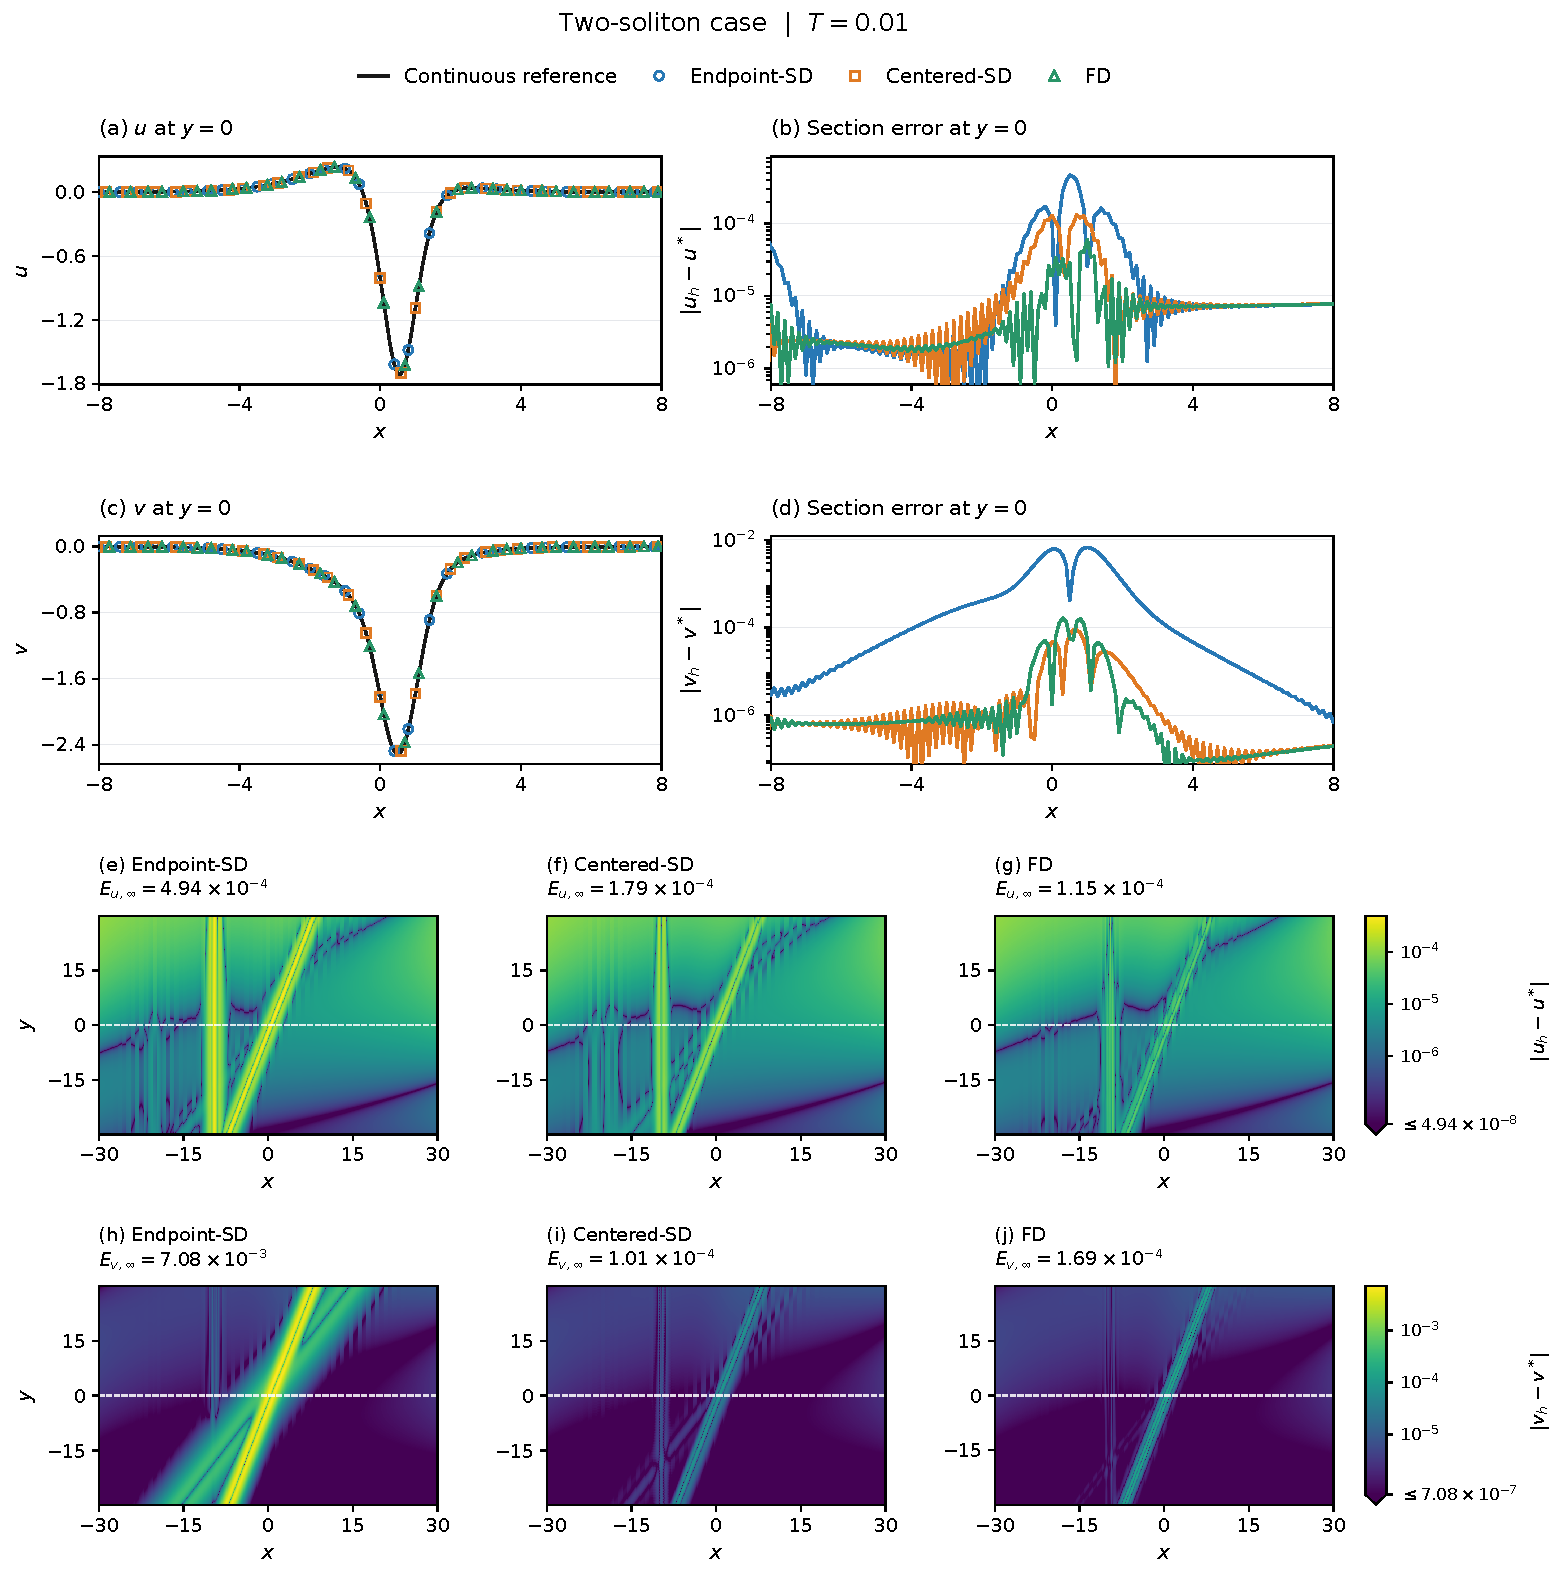
\includegraphics[width=\linewidth,trim=0 177.383bp 0 400.500bp,clip]{images/figure-06.pdf}\par
\noindent\begin{minipage}{\linewidth}
\noindent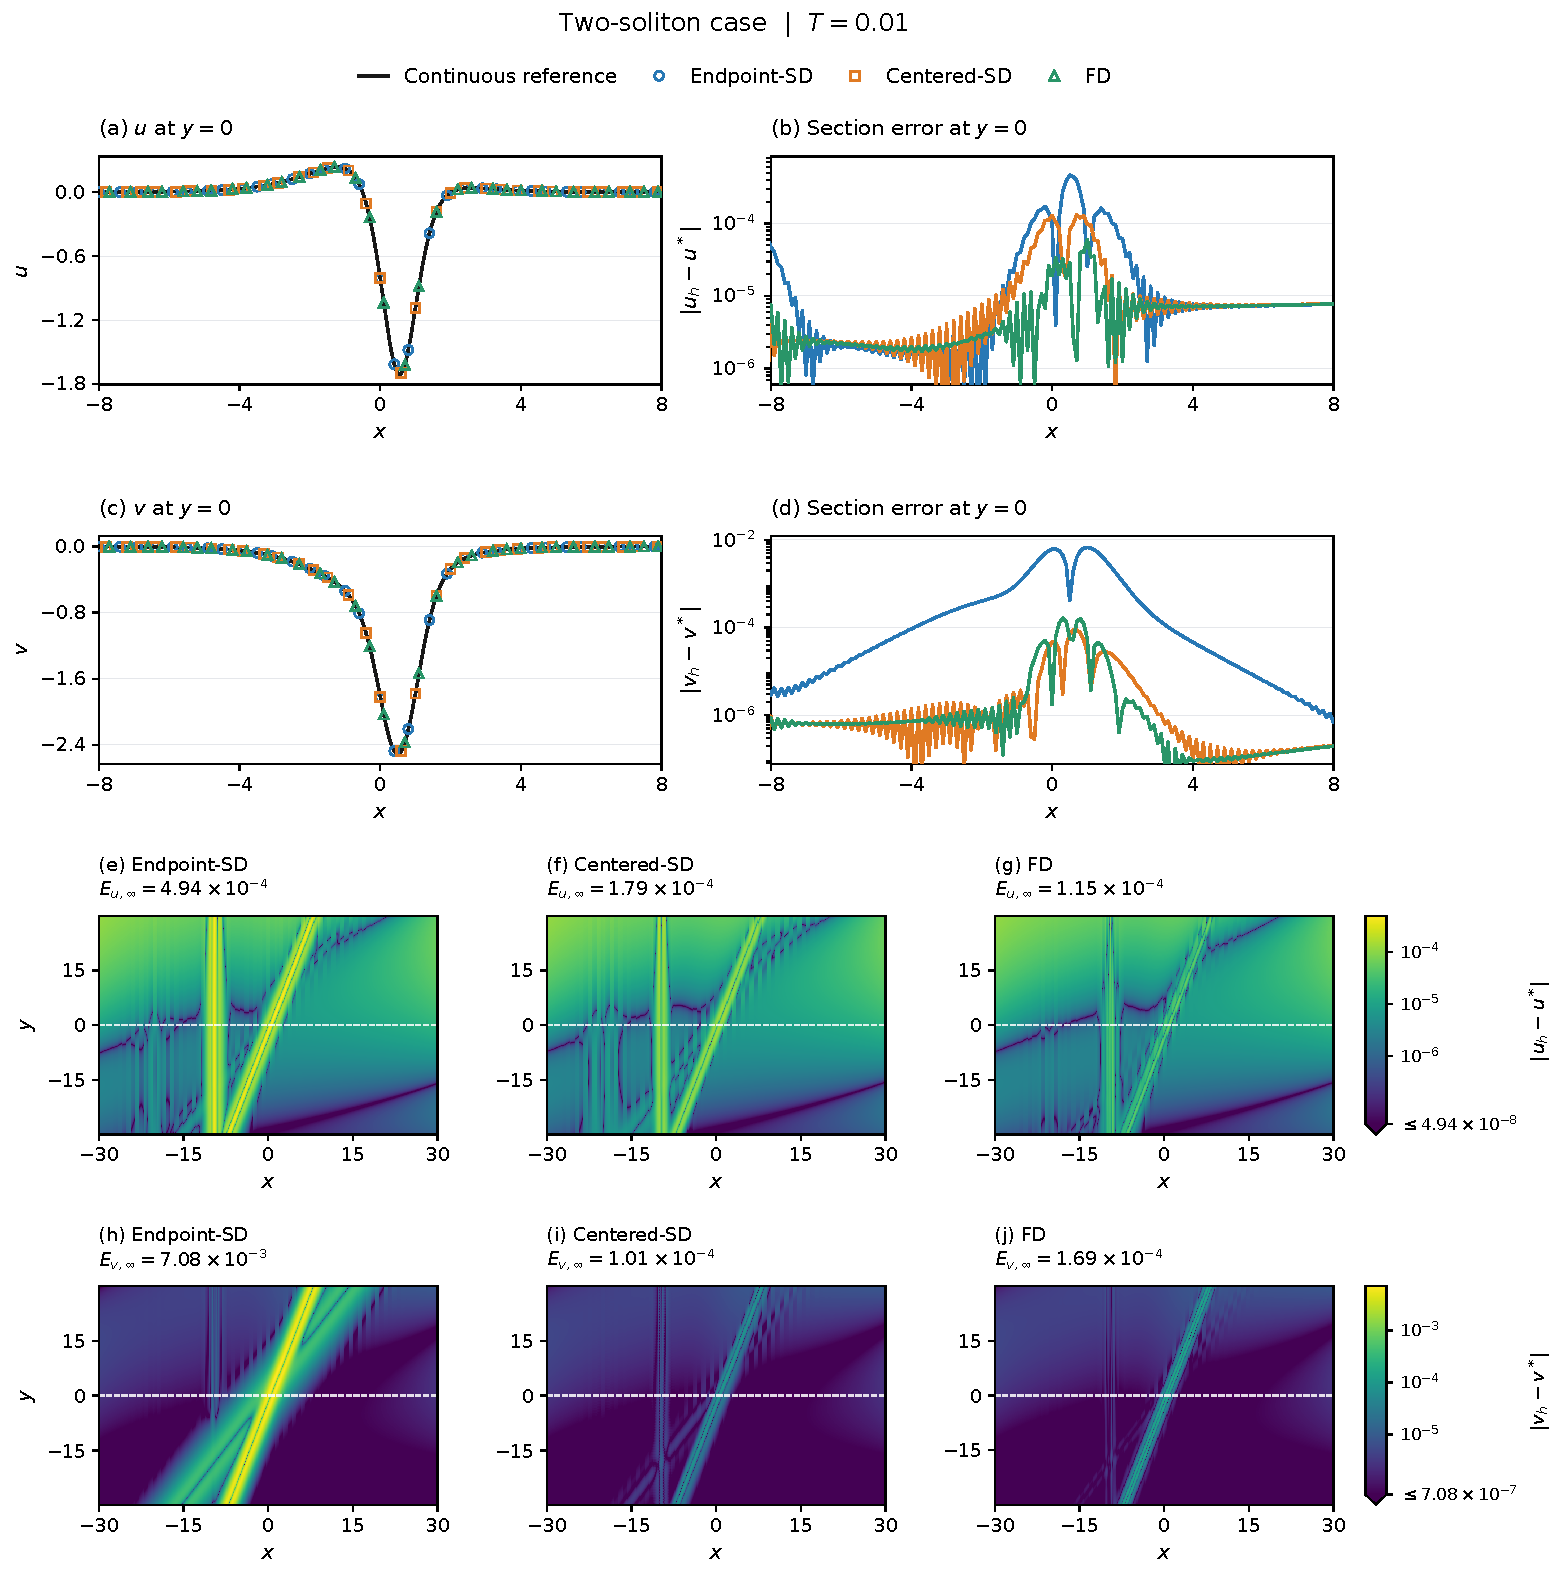
\includegraphics[width=\linewidth,trim=0 0.000bp 0 579.000bp,clip]{images/figure-06.pdf}\par
\captionof*{figure}{\textbf{Figure 6.} Two-soliton case at \(T=0.01\). Panels (a,c) compare the continuous \(y=0\) profiles with numerical symbols; panels (b,d) show the absolute errors along that section. The lower rows show the \(u\) and \(v\) error maps, with columns for Endpoint-SD, Centered-SD and FD. Each row uses one logarithmic color scale; values at or below its lower limit, including zero, share the darkest color, as indicated by the \(\leq\) label on the colorbar. Panel maxima refer to the full table region. The sections focus on \(x\in[-8,8]\), while the maps retain \([-30,30]\).}
\end{minipage}







\subsubsection*{Gaussian and sinusoidal cases}

In the smooth, small-amplitude Gaussian (Figure 7) and sinusoidal (Figure 8) tests, the field gradients are much milder and the terminal error ordering at \(T=0.01\) follows the initial derivative defects of Table 2. Endpoint-SD gives the smallest \(u\) error, while Centered-SD lies between Endpoint-SD and FD in \(u\) and produces the smallest \(v\) error in both tests. Specifically, Centered-SD reduces \(E_v\) to \(6.967\times10^{-9}\) in the Gaussian case (about \(3.2\) times smaller than FD and \(87\) times smaller than Endpoint-SD) and to \(4.706\times10^{-9}\) in the sinusoidal case (\(3.5\) times smaller than FD and \(60\) times smaller than Endpoint-SD). Because the exact second field remains constant at \(v=4\) along the symmetry line \(y=0\), the cross-sectional \(v\) error along \(y=0\) is near machine precision, while the heatmaps show how the errors distribute symmetrically across the upper and lower halves of the strip.

Figure 7(a) shows the Gaussian section as a smooth positive hump, with all three sets of numerical symbols following the reference curve. Panel (b) resolves the much smaller differences between them as several error lobes across the hump. The second field is constant along \(y=0\) in panel (c), and the enlarged vertical scale in panel (d) displays section errors of order \(10^{-12}\). The heatmaps below show the transverse variation that this central section does not sample: the \(v\) error grows away from the symmetry line and forms corresponding patterns in the upper and lower halves of the strip.

\FloatBarrier
\noindent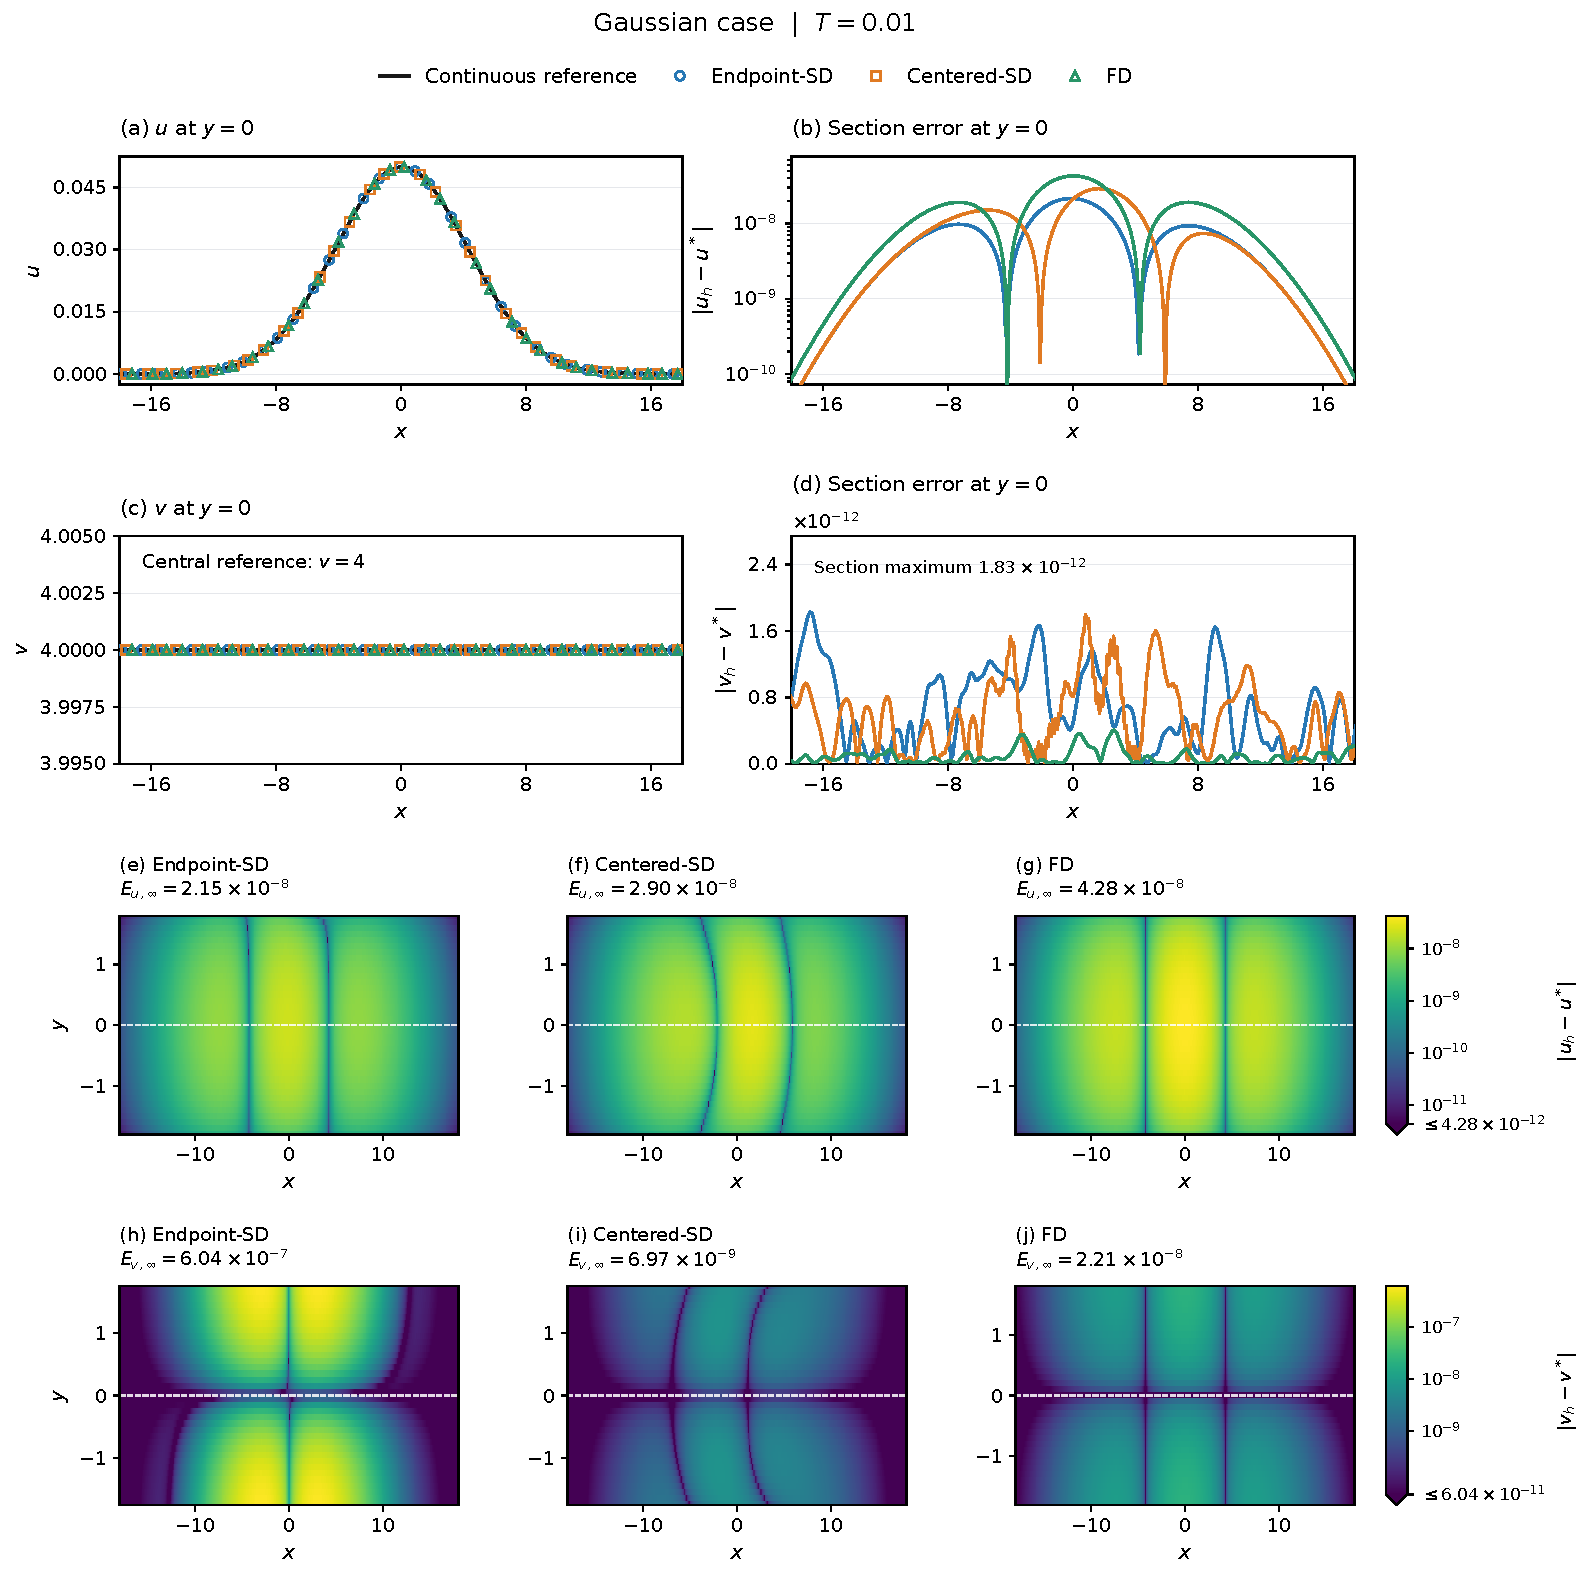
\includegraphics[width=\linewidth,trim=0 537.883bp 0 0.000bp,clip]{images/figure-07.pdf}\par
\noindent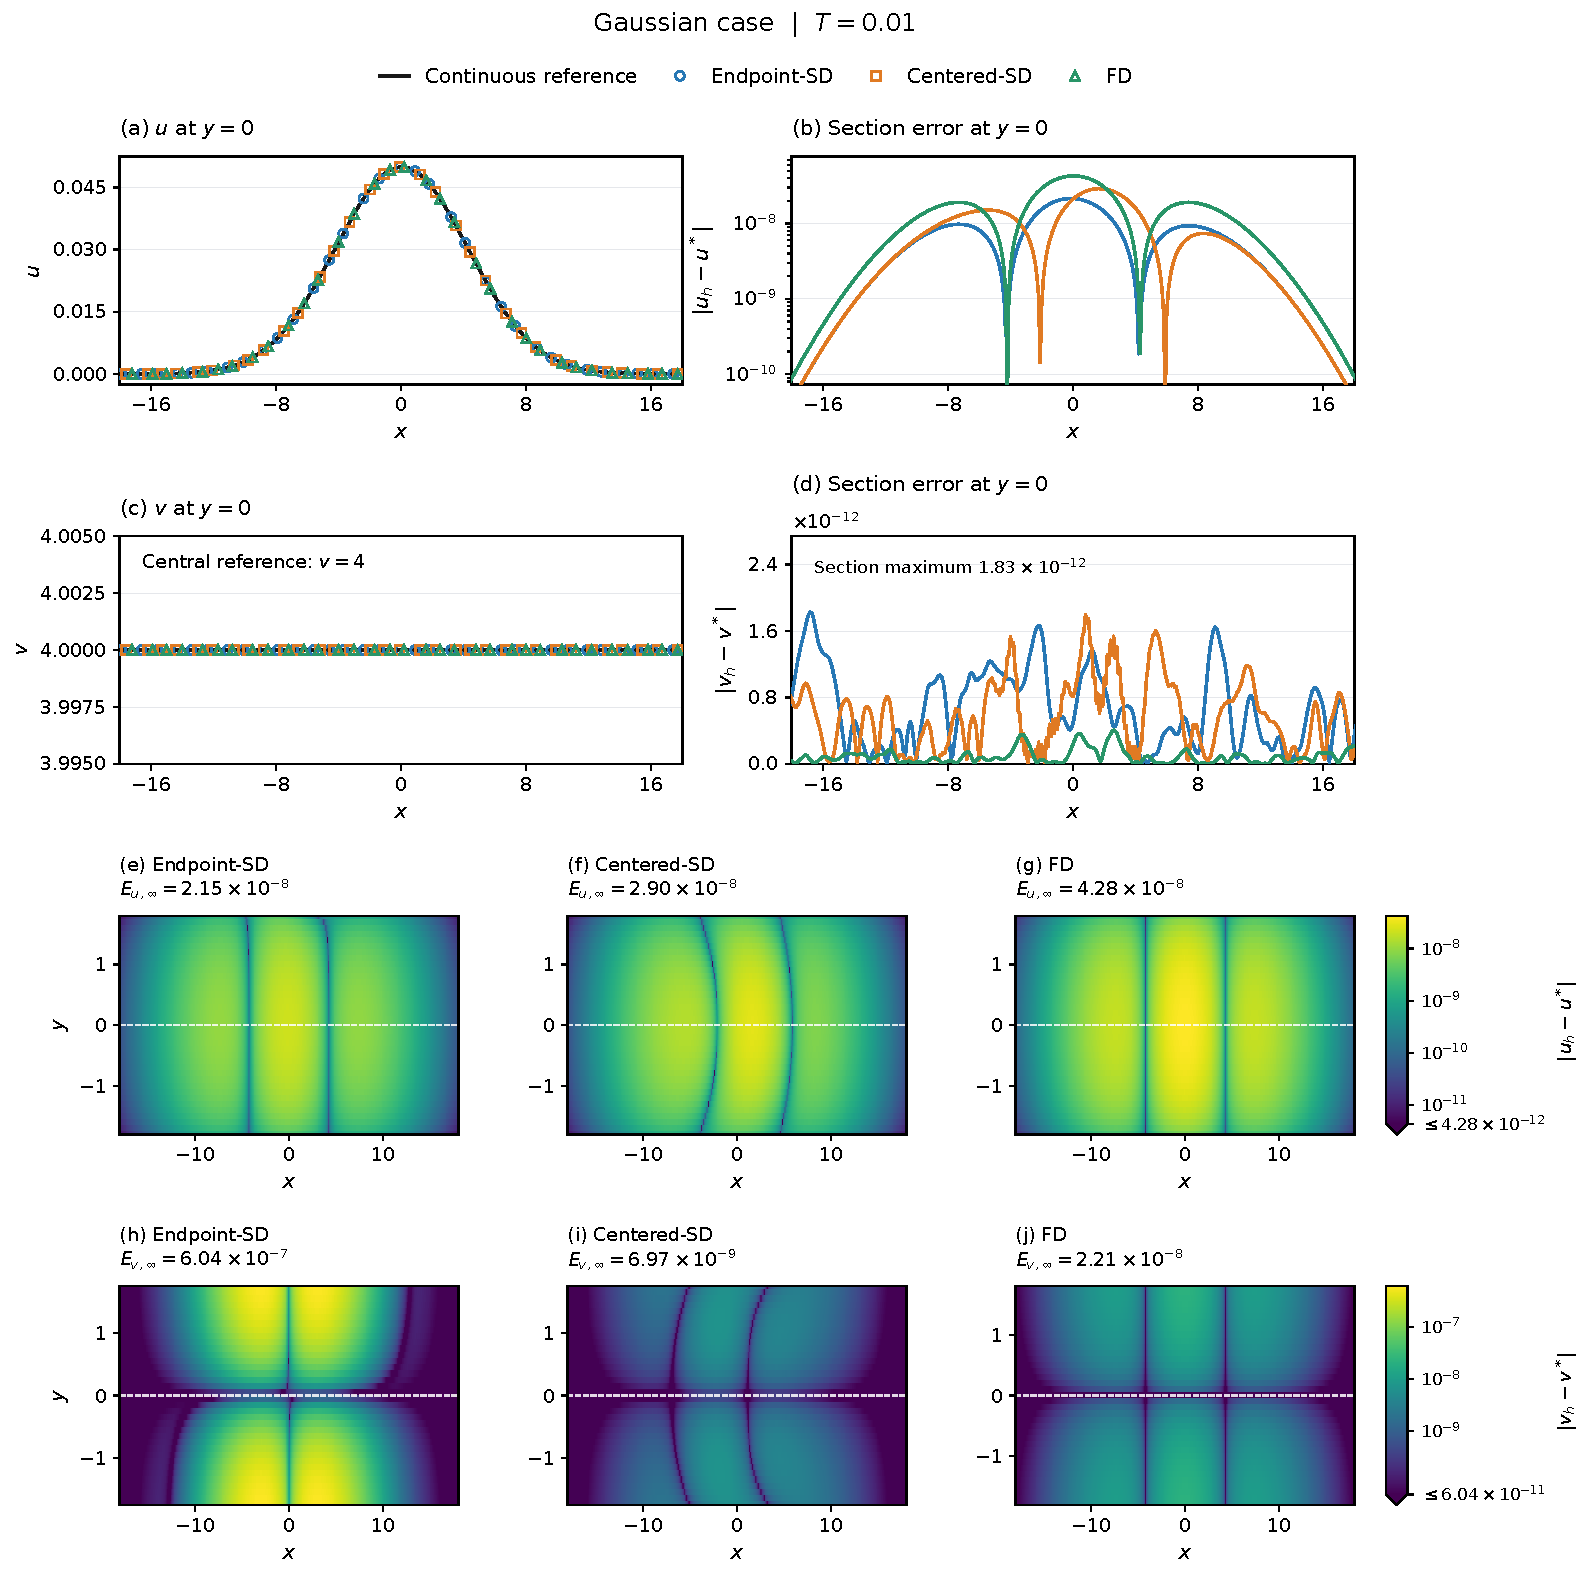
\includegraphics[width=\linewidth,trim=0 355.883bp 0 218.500bp,clip]{images/figure-07.pdf}\par
\noindent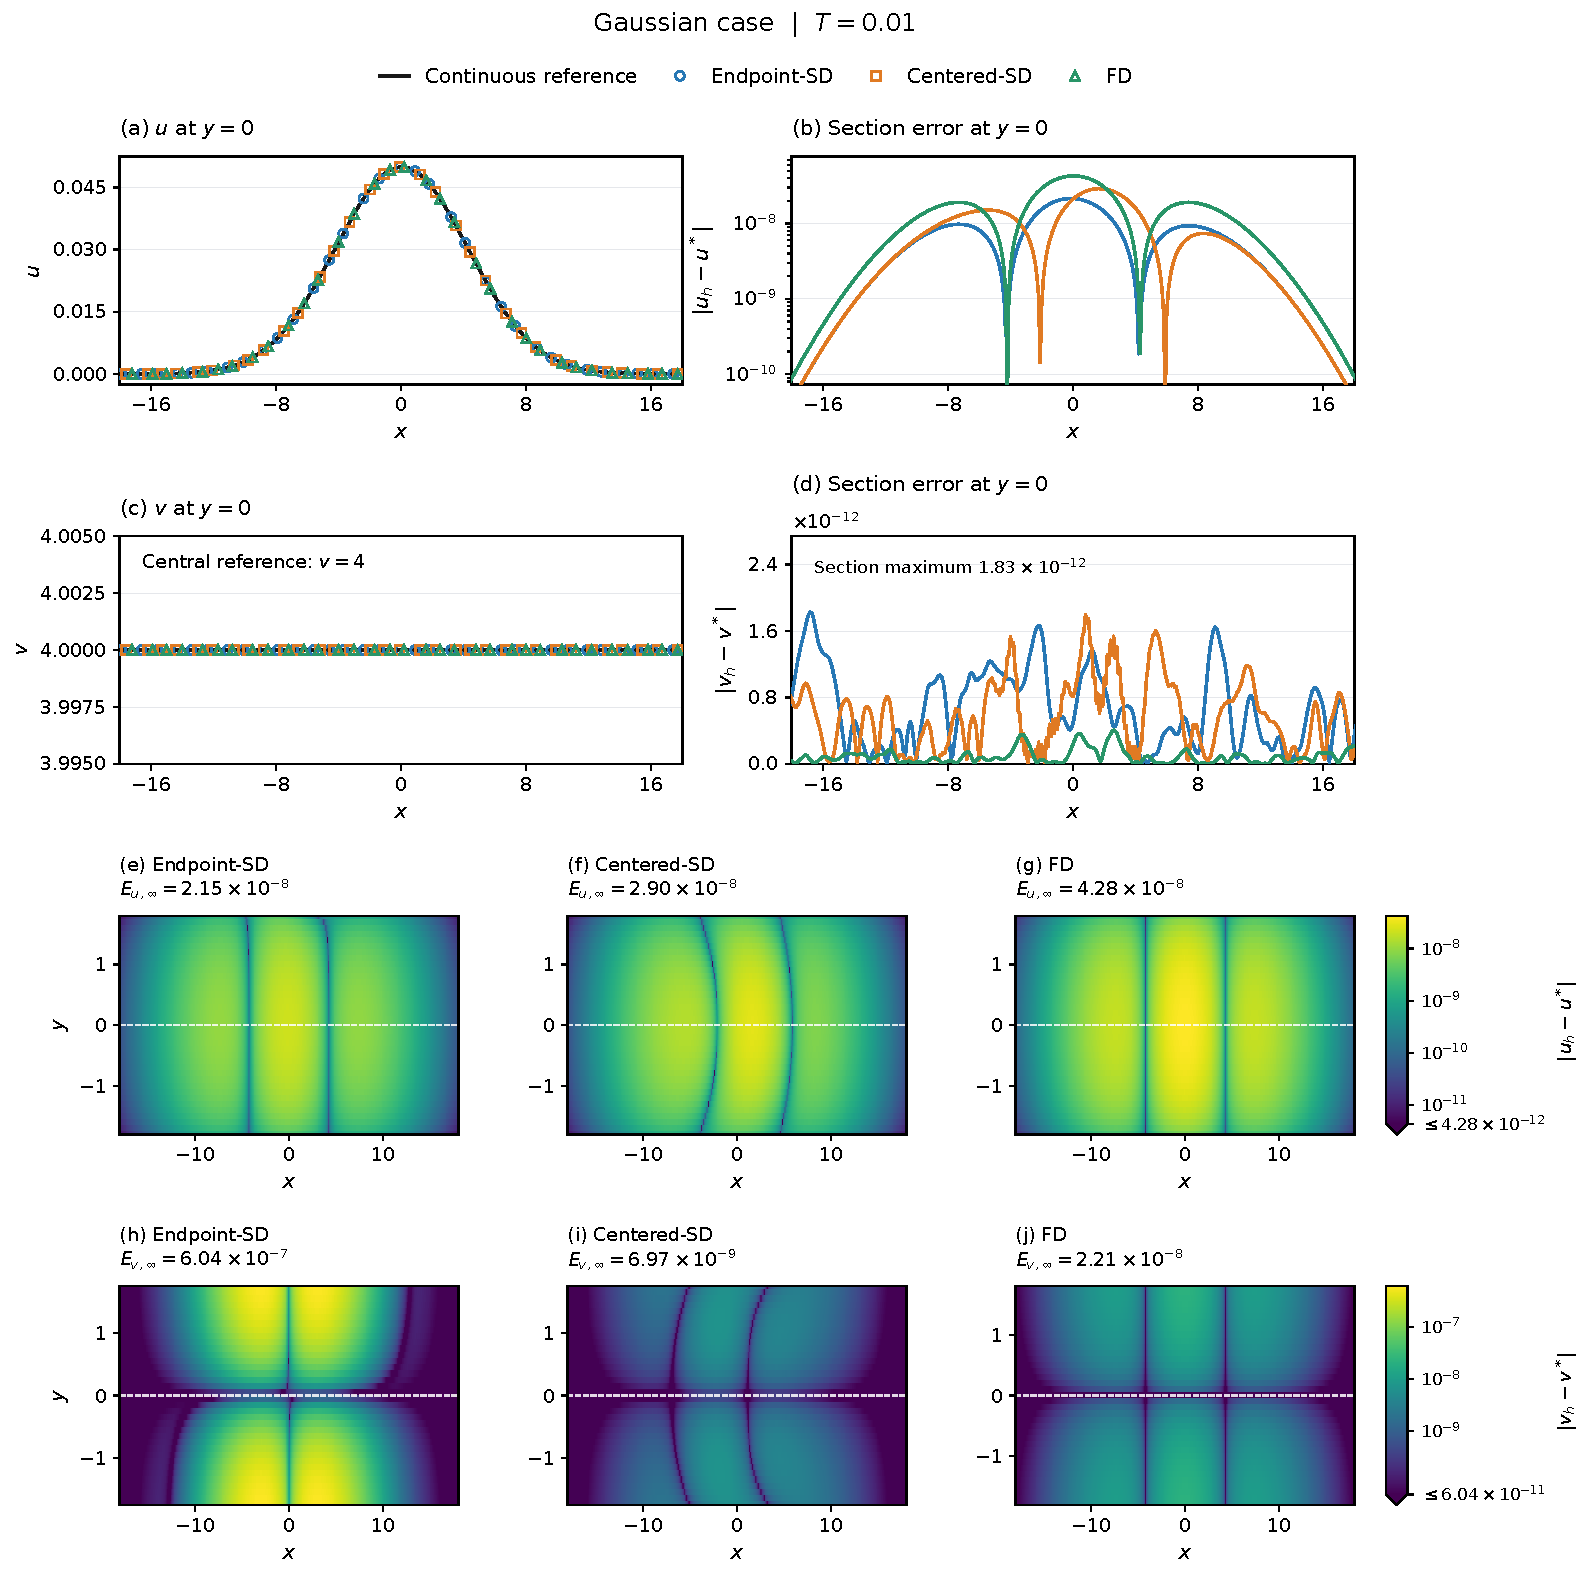
\includegraphics[width=\linewidth,trim=0 177.383bp 0 400.500bp,clip]{images/figure-07.pdf}\par
\noindent\begin{minipage}{\linewidth}
\noindent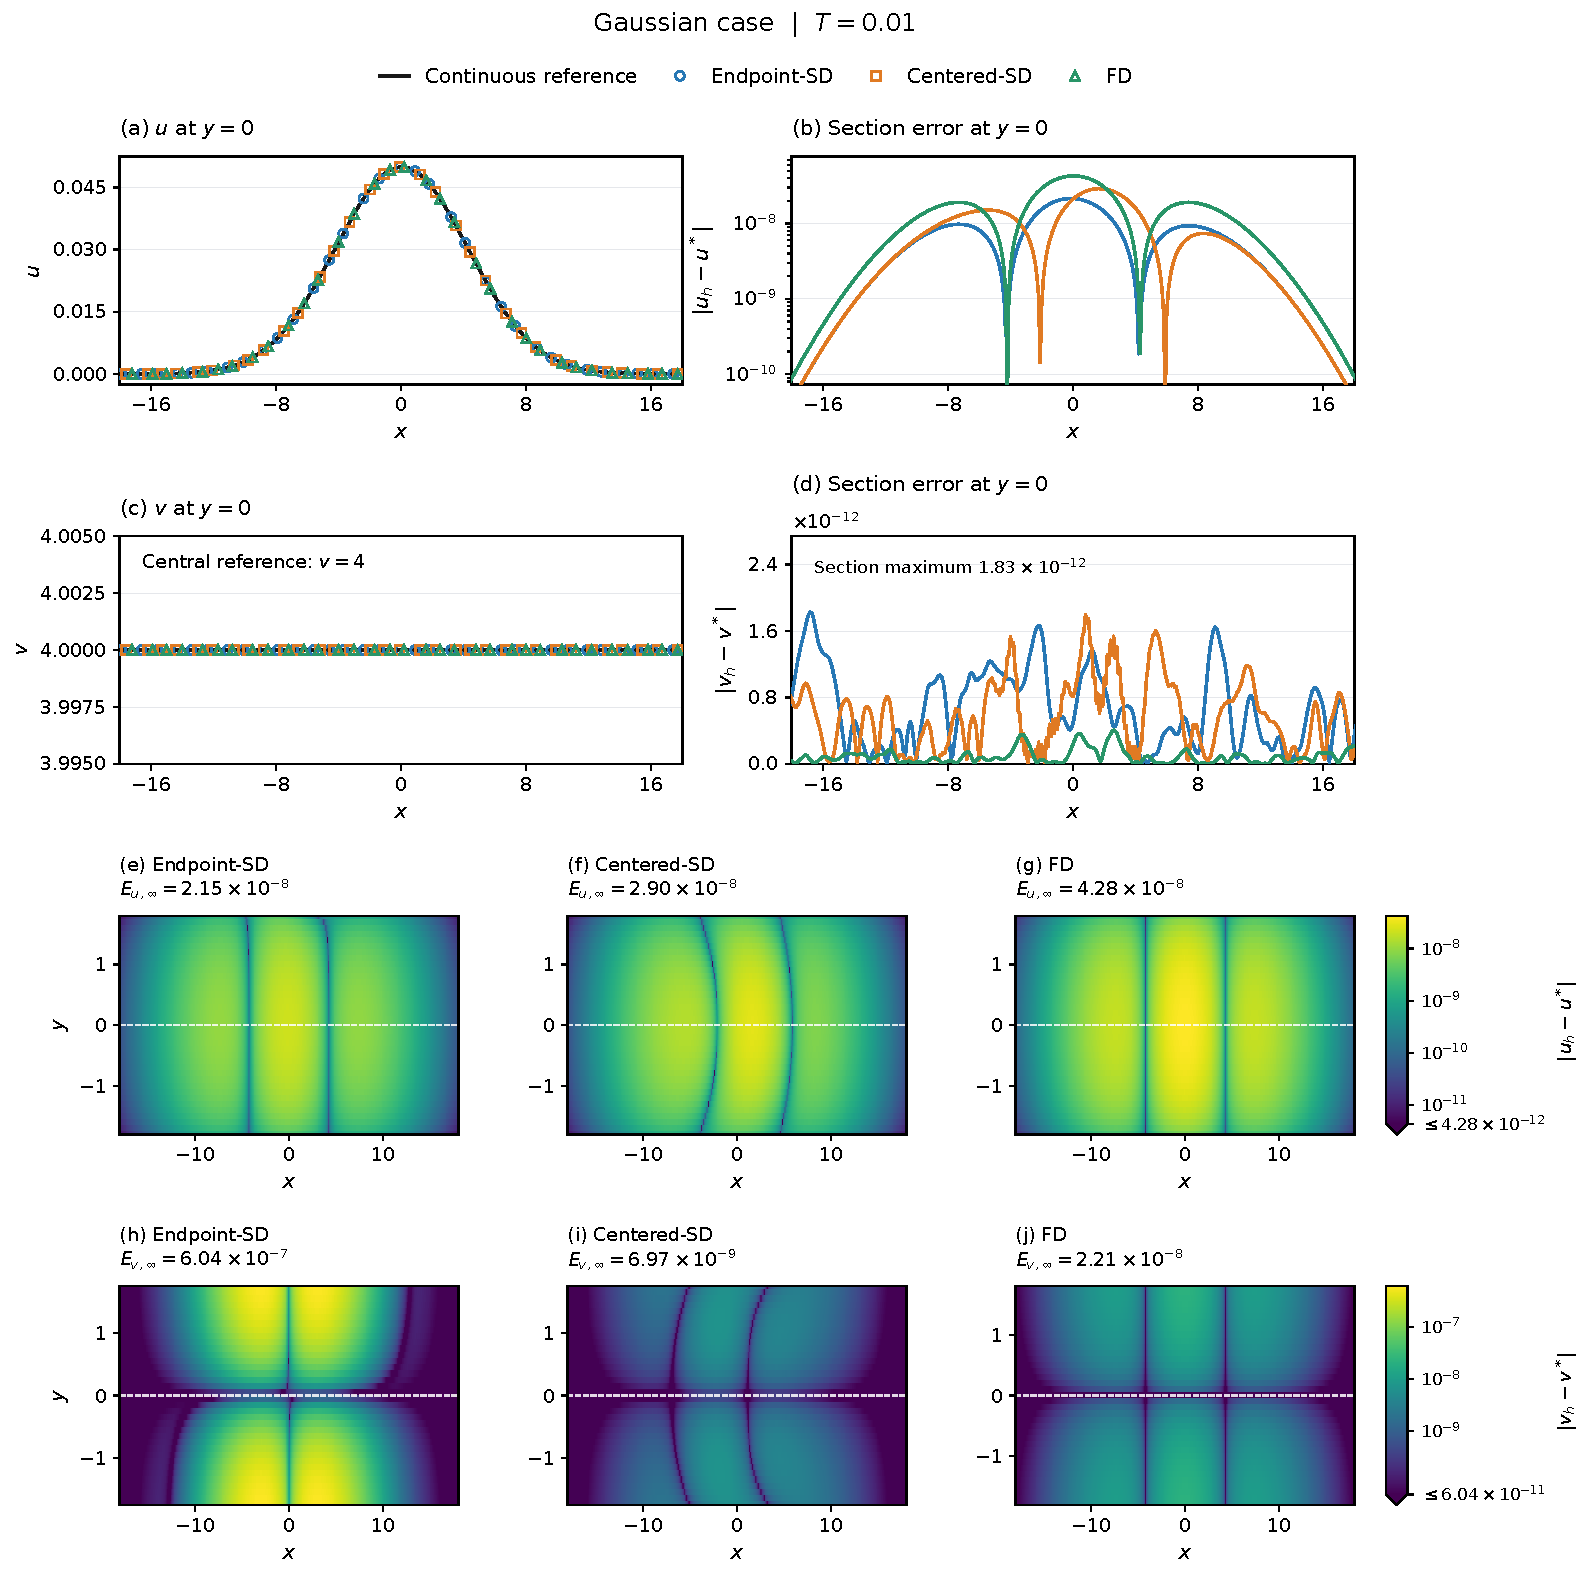
\includegraphics[width=\linewidth,trim=0 0.000bp 0 579.000bp,clip]{images/figure-07.pdf}\par
\captionof*{figure}{\textbf{Figure 7.} Gaussian case at \(T=0.01\). Panels (a,c) compare the continuous \(y=0\) profiles with numerical symbols; panels (b,d) show the absolute errors along that section. The lower rows show the \(u\) and \(v\) error maps, with columns for Endpoint-SD, Centered-SD and FD. Each row uses one logarithmic color scale; values at or below its lower limit, including zero, share the darkest color, as indicated by the \(\leq\) label on the colorbar. Panel maxima refer to the full table region. The display window is \([-18,18]\); the table uses the full periodic interval \([-96,96)\). The exact central second field is \(v(x,0,t)=4\).}
\end{minipage}





Figure 8(a) presents the sinusoidal section, with a positive crest near the center and negative values toward the ends of the displayed interval. The numerical symbols follow this alternating profile, while panel (b) separates their section errors. As in the Gaussian test, \(v\) is constant on \(y=0\) and its section error remains of order \(10^{-12}\). In the heatmaps, the errors vary along both spatial directions, forming repeated bands and lobes. Reading the sections together with these maps shows how close agreement on the central line accompanies a nonuniform error distribution across the strip.

\FloatBarrier
\noindent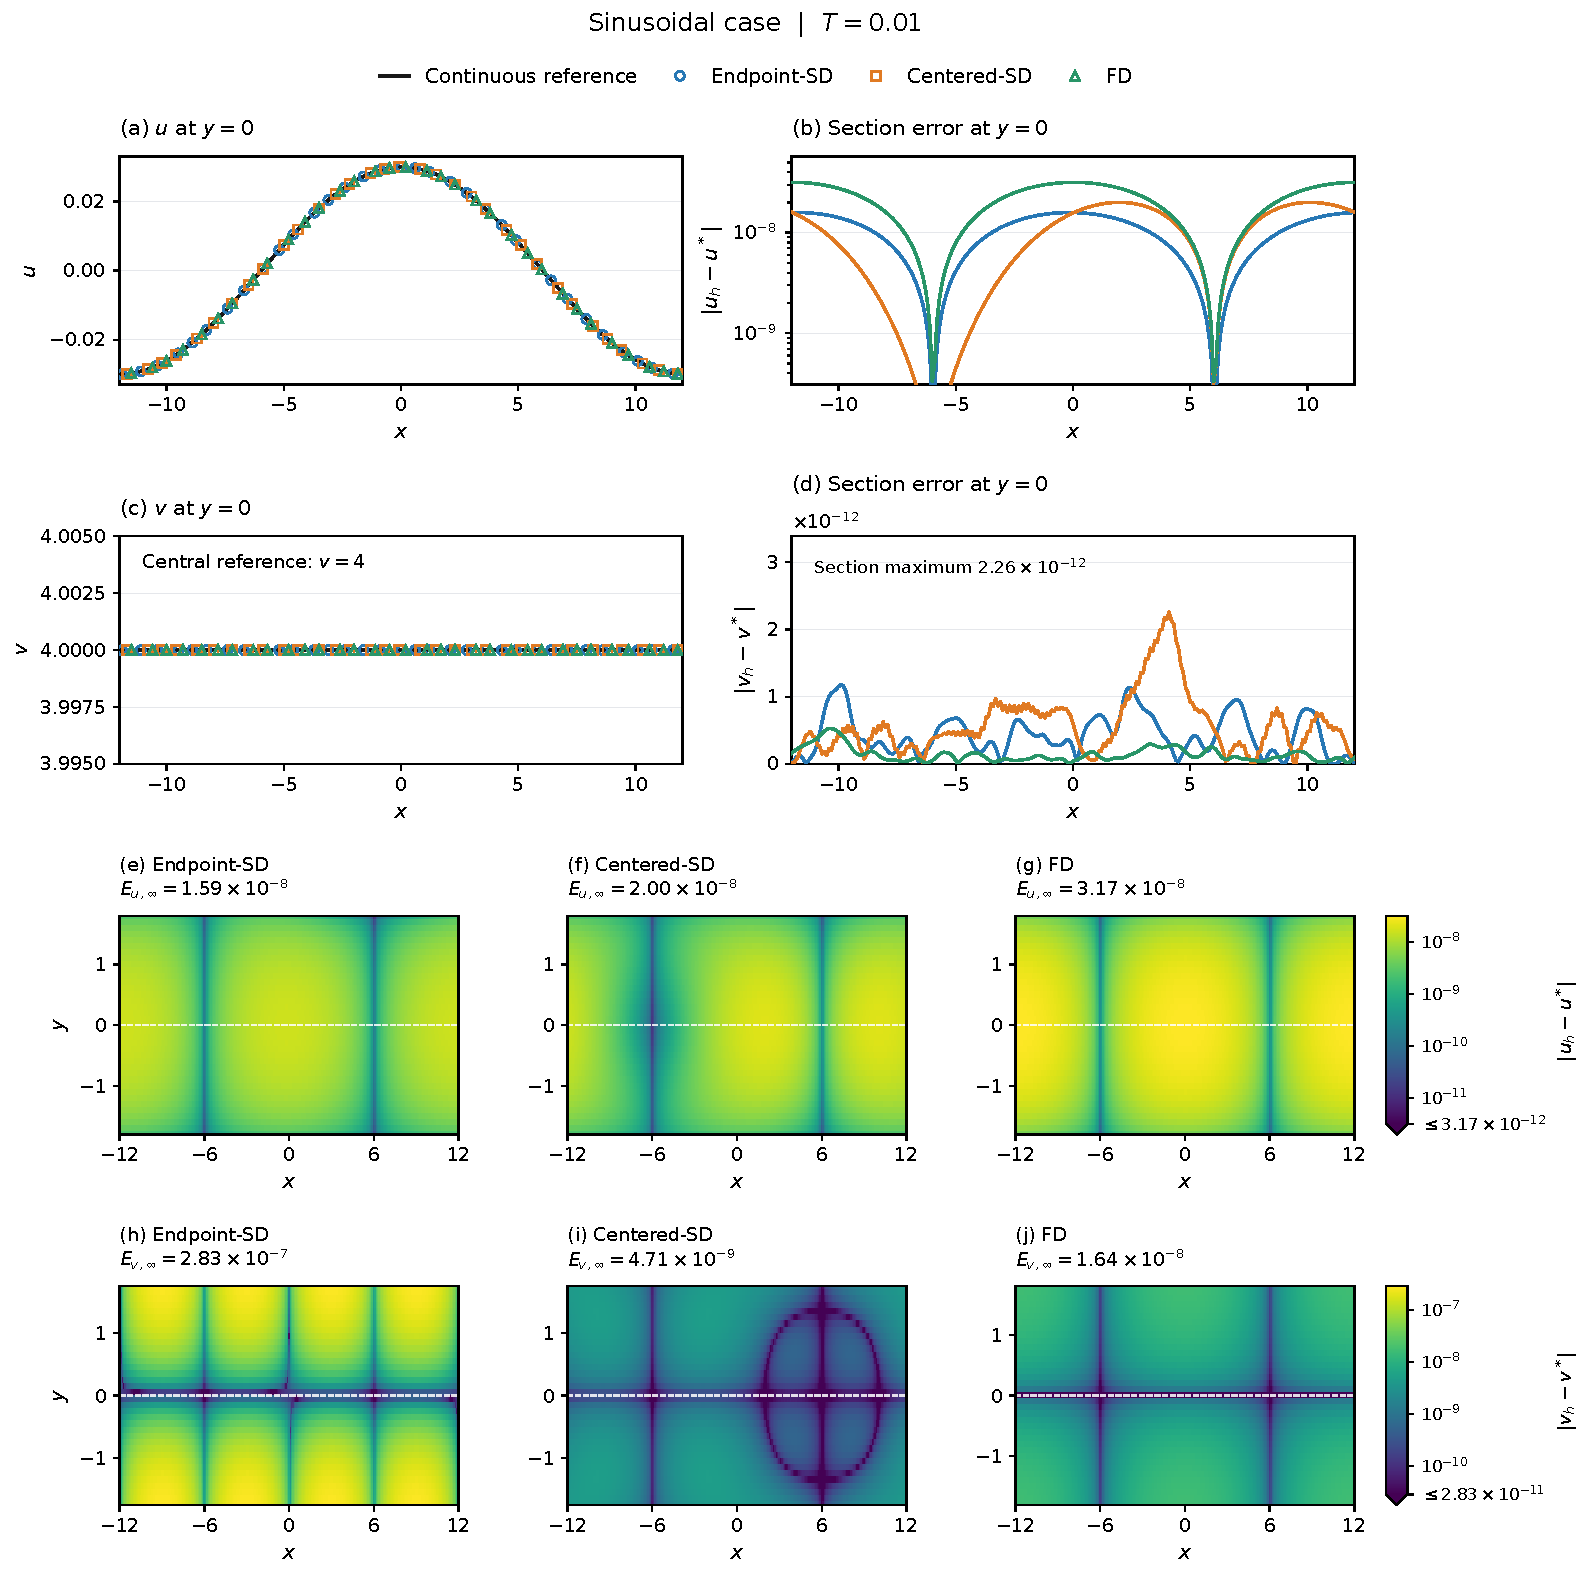
\includegraphics[width=\linewidth,trim=0 537.883bp 0 0.000bp,clip]{images/figure-08.pdf}\par
\noindent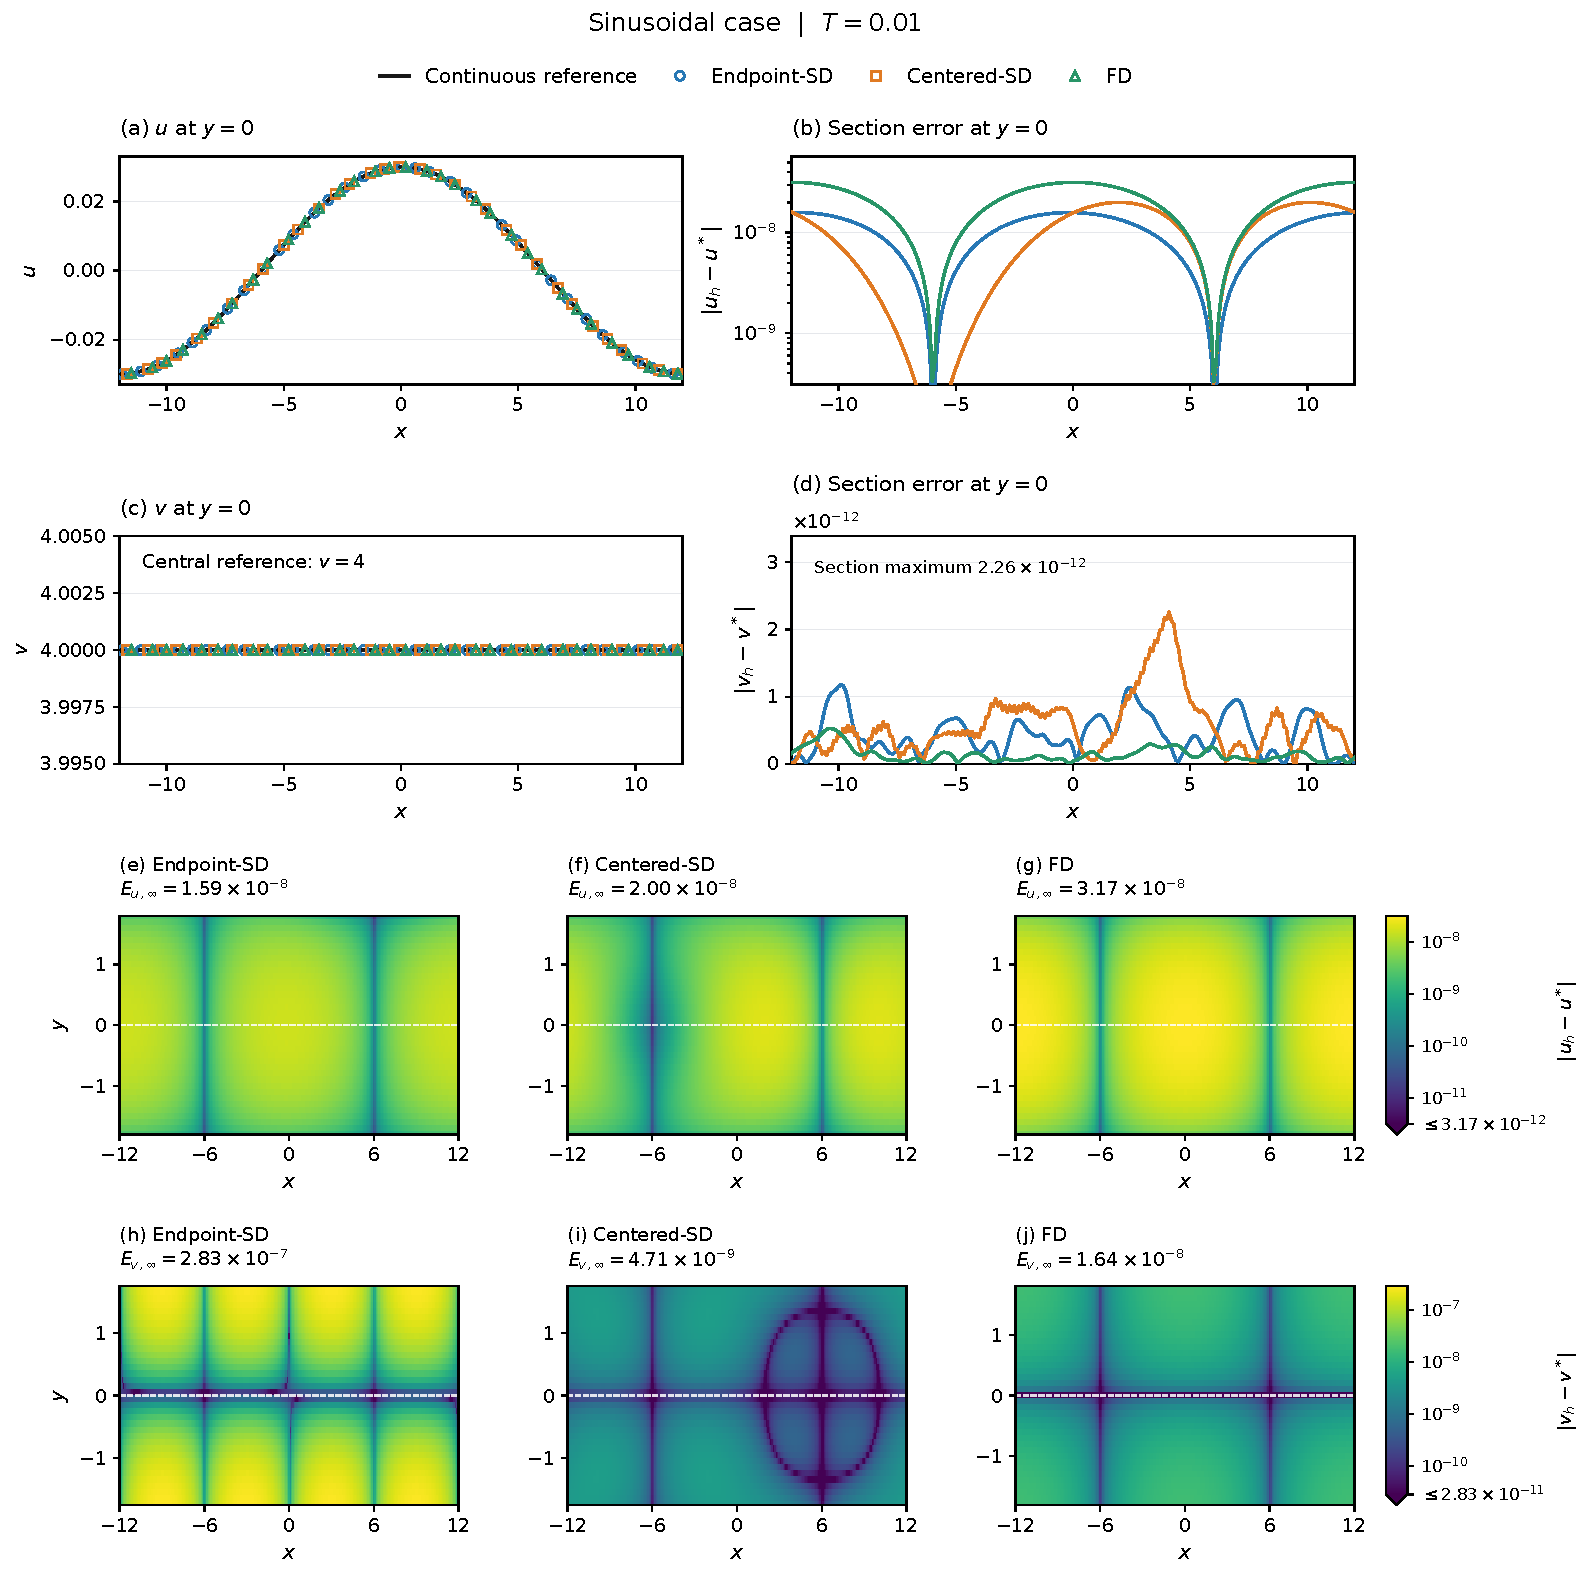
\includegraphics[width=\linewidth,trim=0 355.883bp 0 218.500bp,clip]{images/figure-08.pdf}\par
\noindent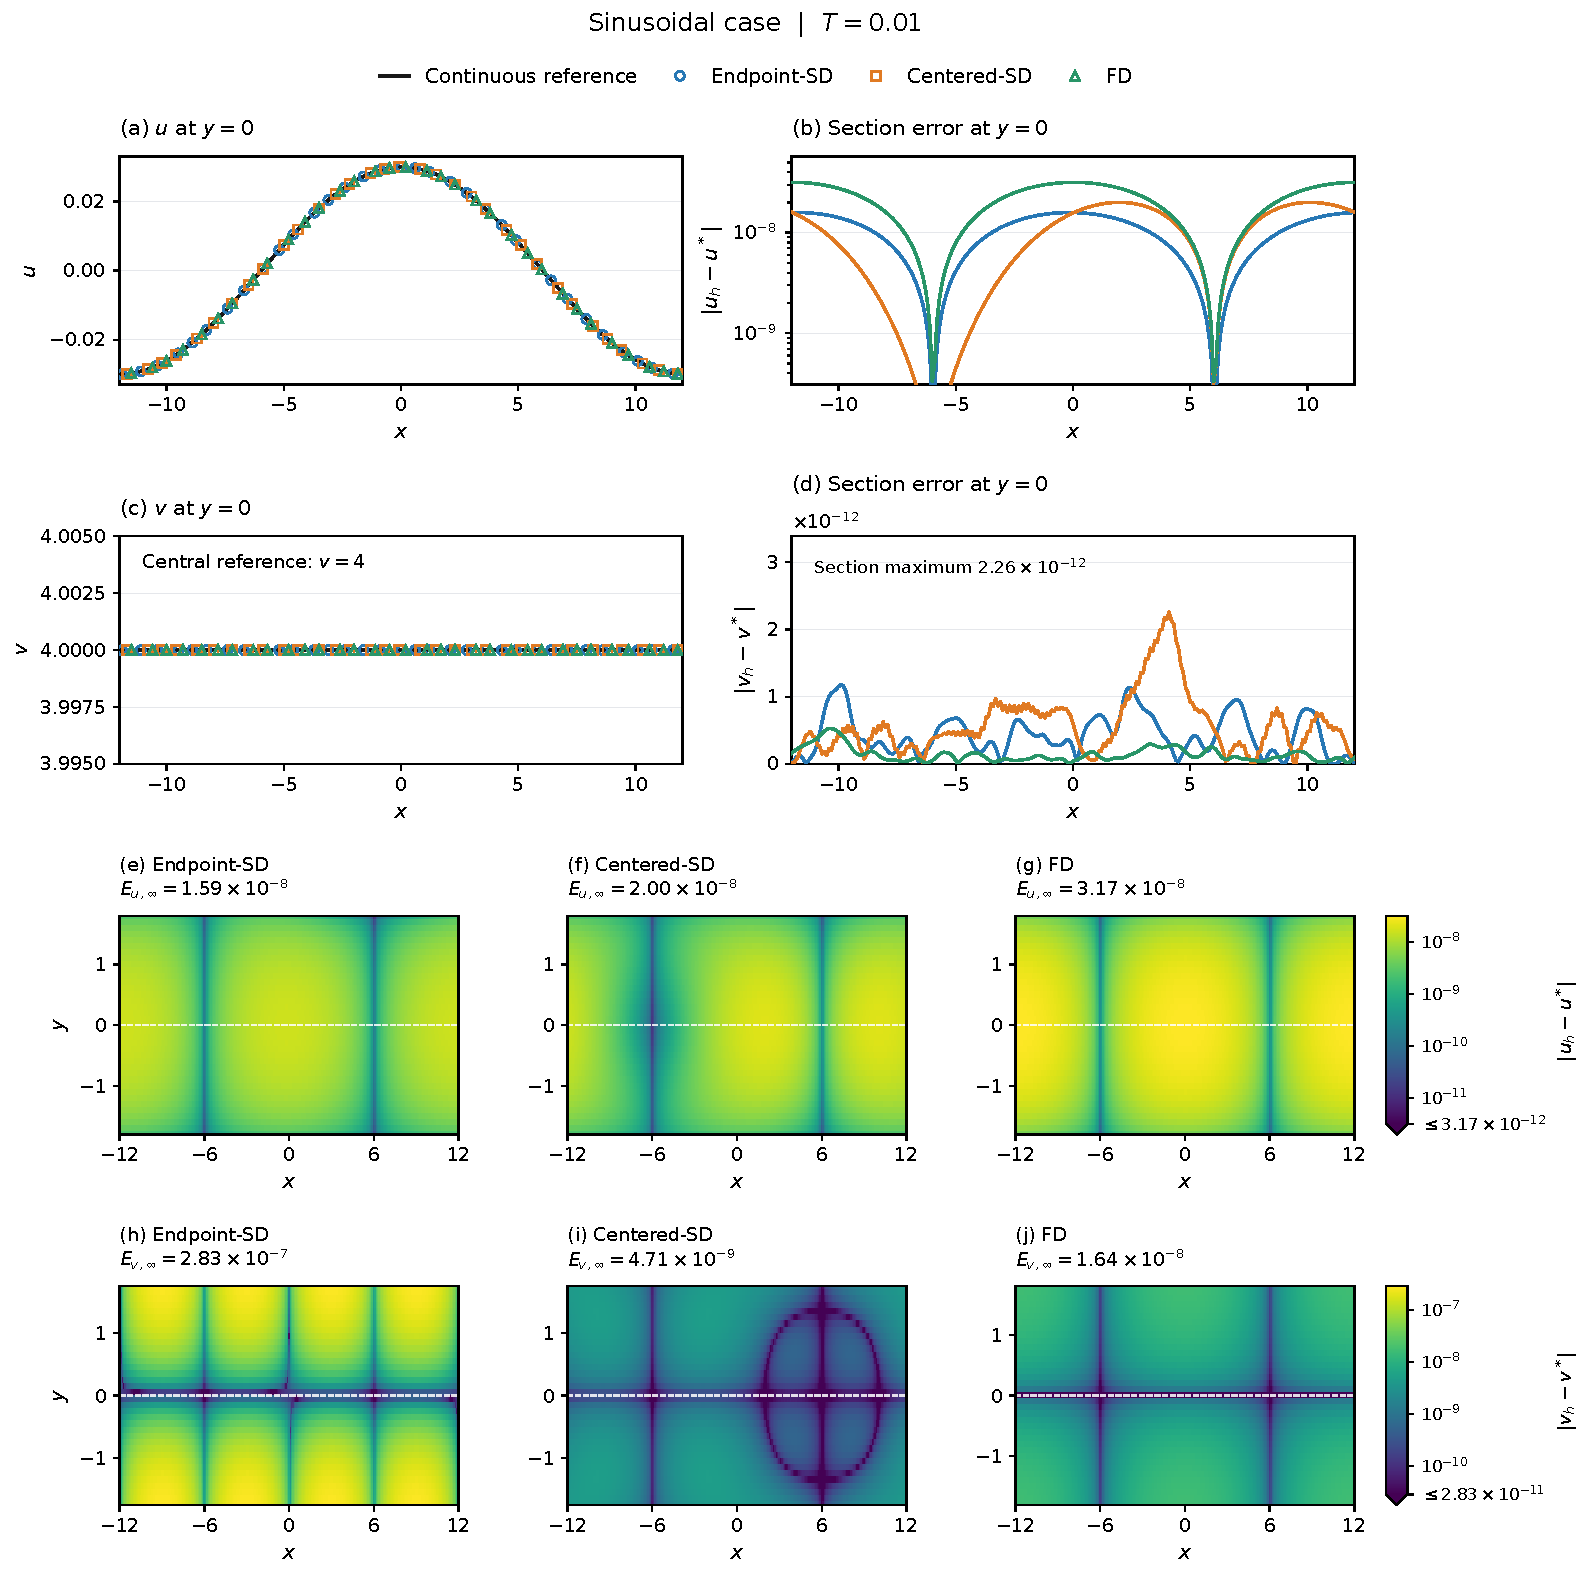
\includegraphics[width=\linewidth,trim=0 177.383bp 0 400.500bp,clip]{images/figure-08.pdf}\par
\noindent\begin{minipage}{\linewidth}
\noindent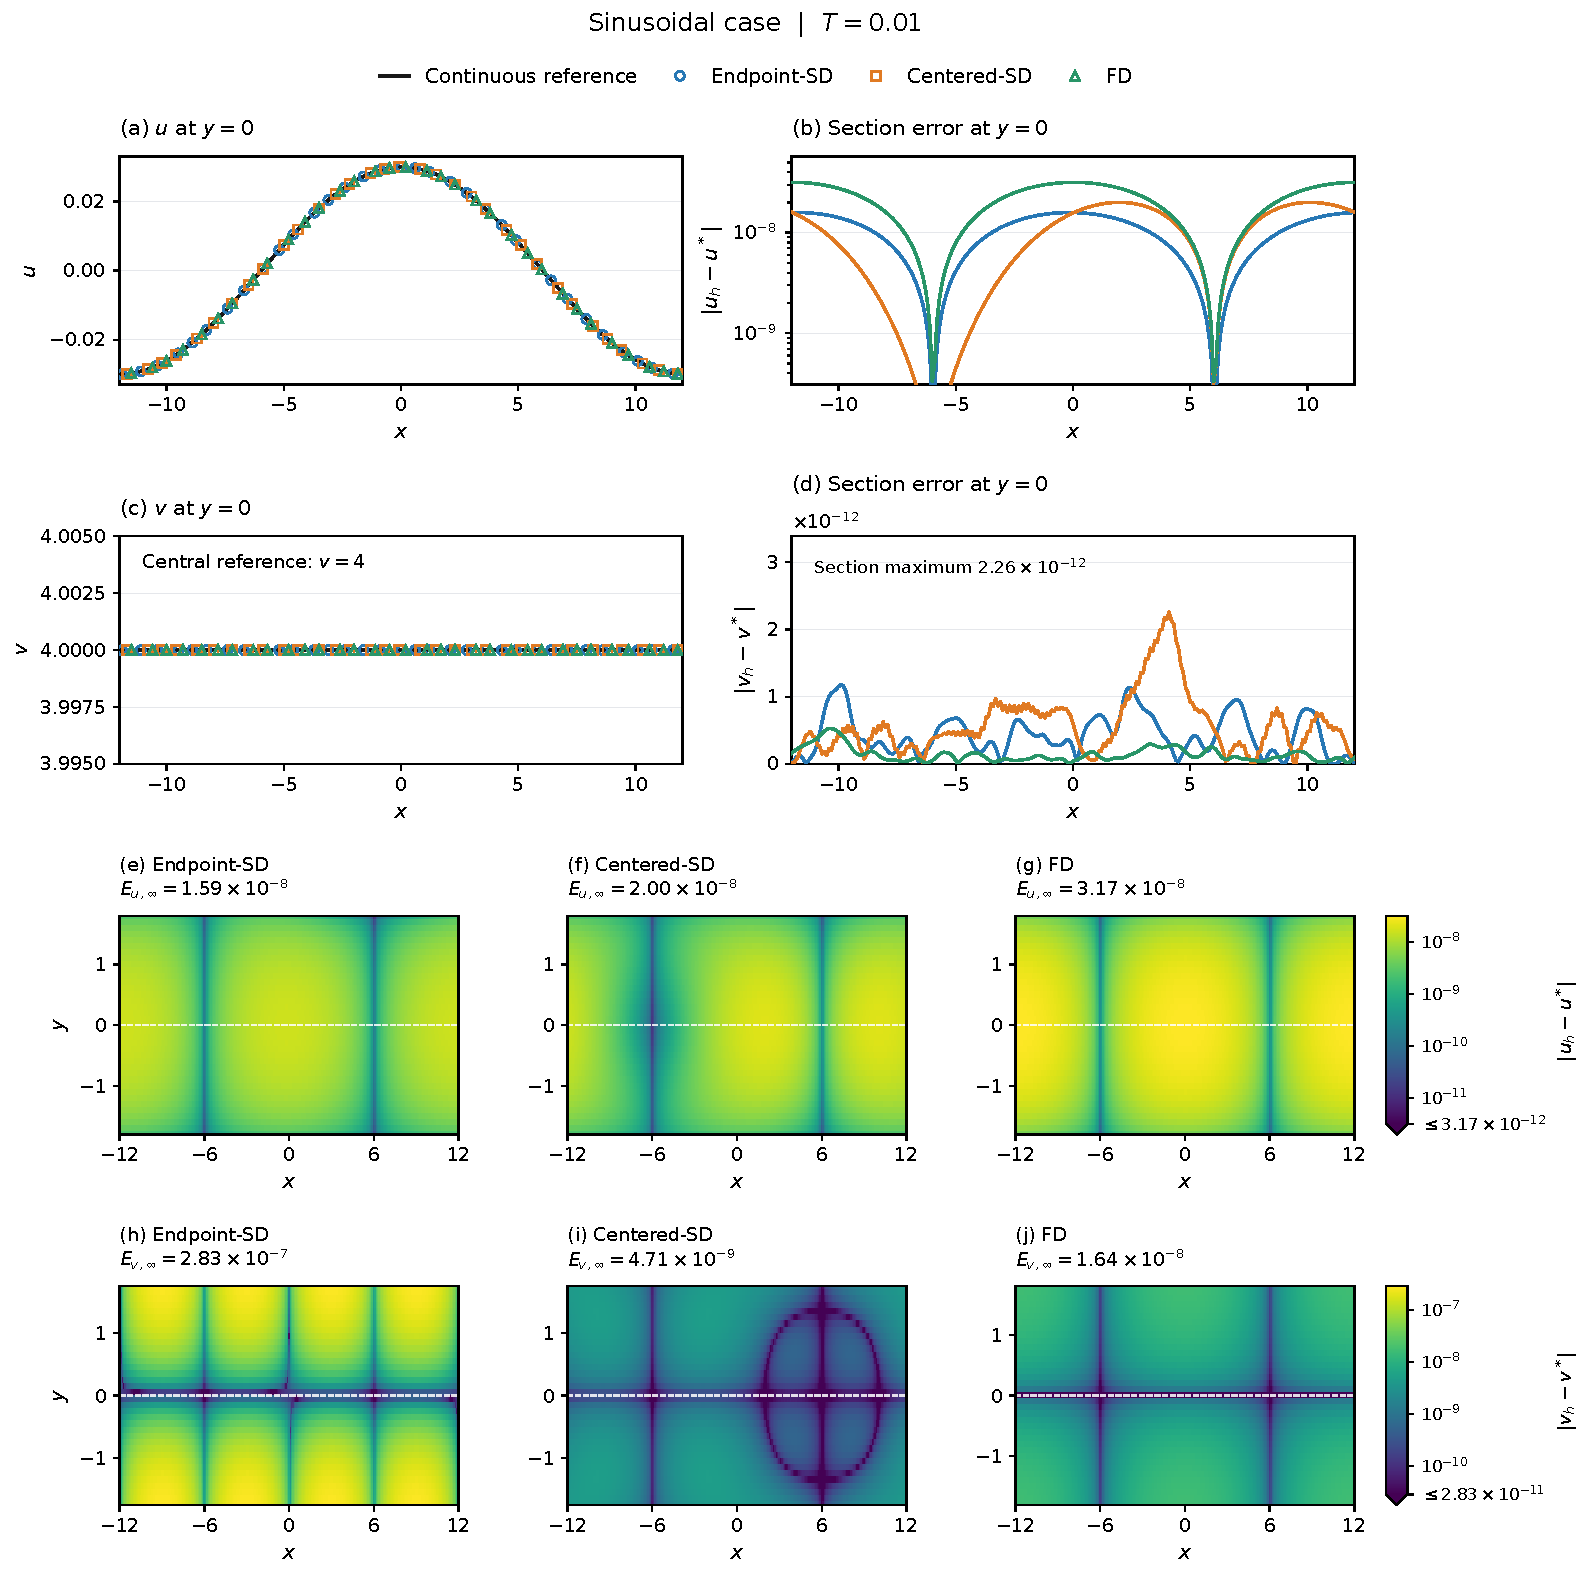
\includegraphics[width=\linewidth,trim=0 0.000bp 0 579.000bp,clip]{images/figure-08.pdf}\par
\captionof*{figure}{\textbf{Figure 8.} Sinusoidal case at \(T=0.01\). Panels (a,c) compare the continuous \(y=0\) profiles with numerical symbols; panels (b,d) show the absolute errors along that section. The lower rows show the \(u\) and \(v\) error maps, with columns for Endpoint-SD, Centered-SD and FD. Each row uses one logarithmic color scale; values at or below its lower limit, including zero, share the darkest color, as indicated by the \(\leq\) label on the colorbar. Panel maxima refer to the full table region. The display window is \([-12,12]\); the table uses the full periodic interval \([-96,96)\). The exact central second field is \(v(x,0,t)=4\).}
\end{minipage}





The four tests distinguish the accuracy of the initial time derivatives from that of the fields after evolution. Endpoint-SD retains its initial advantage in the first component on the Gaussian and sinusoidal backgrounds, while Centered-SD gives smaller terminal errors in both fields in the soliton tests. The initial approximation of one component must therefore be considered together with the evolution of the coupled fields.

The consistency analysis identifies the truncation terms introduced by each lattice arrangement. During evolution, the coupling provides a route for these errors to affect the other component; in particular, the \(v_{xx}\) term links the approximation of \(v\) to the computed \(u\) field. The change in error ordering in the soliton tests is consistent with this coupling. Initial derivative errors and evolved field errors thus provide complementary measures of the spatial approximation.

\FloatBarrier
\subsection*{5.3 Comparison of time integrators}

The preceding comparison follows spatial approximation errors through the coupled evolution using RK4. We now keep Centered-SD fixed and vary the time integrator to examine how temporal approximation changes this behavior. Forward Euler, classical RK4, and Crank–Nicolson use the same exact initial fields, spatial operators and boundary data on the uniform grid with \(h=\Delta x=0.1\), and advance to \(T=0.01\) with \(\Delta t=10^{-4}\). We compare both the terminal errors and their time histories to see how the additional temporal error affects each physical component.

\begin{table}[!htbp]
\centering
\caption*{Table 4. Physical-field errors at T = 0.01 for Centered-SD with forward Euler, RK4 and Crank–Nicolson at h = \(\Delta\)x = 0.1 and \(\Delta\)t = 10\textsuperscript{-}\textsuperscript{4}. Values are rounded to four significant digits; some RK4 and Crank–Nicolson entries therefore coincide. Additional digits, signed differences and the smaller recorded error are given in Appendix D, Table 8. Bold values indicate the smallest error among the three integrators, determined before rounding.}
\small
\setlength{\tabcolsep}{4pt}
\renewcommand{\arraystretch}{1.22}
\begin{tabularx}{\linewidth}{YYYYYYY}
\toprule
Case & \multicolumn{2}{>{\raggedright\arraybackslash}p{2\dimexpr\linewidth/7-2\tabcolsep\relax}}{Forward Euler} & \multicolumn{2}{>{\raggedright\arraybackslash}p{2\dimexpr\linewidth/7-2\tabcolsep\relax}}{RK4} & \multicolumn{2}{>{\raggedright\arraybackslash}p{2\dimexpr\linewidth/7-2\tabcolsep\relax}}{Crank–Nicolson} \\
 & \(E_u\) & \(E_v\) & \(E_u\) & \(E_v\) & \(E_u\) & \(E_v\) \\
\midrule
One-soliton & \textbf{1.664 \(\times\) 10\textsuperscript{-4}} & 8.026 \(\times\) 10\textsuperscript{-5} & 1.677 \(\times\) 10\textsuperscript{-4} & \textbf{7.734 \(\times\) 10\textsuperscript{-5}} & 1.677 \(\times\) 10\textsuperscript{-4} & 7.734 \(\times\) 10\textsuperscript{-5} \\
Two-soliton & \textbf{1.420 \(\times\) 10\textsuperscript{-4}} & 1.090 \(\times\) 10\textsuperscript{-4} & 1.792 \(\times\) 10\textsuperscript{-4} & \textbf{1.009 \(\times\) 10\textsuperscript{-4}} & 1.805 \(\times\) 10\textsuperscript{-4} & 1.009 \(\times\) 10\textsuperscript{-4} \\
Gaussian & \textbf{5.107 \(\times\) 10\textsuperscript{-9}} & 5.680 \(\times\) 10\textsuperscript{-8} & 2.900 \(\times\) 10\textsuperscript{-8} & \textbf{6.967 \(\times\) 10\textsuperscript{-9}} & 2.900 \(\times\) 10\textsuperscript{-8} & 6.969 \(\times\) 10\textsuperscript{-9} \\
Sinusoidal & \textbf{1.243 \(\times\) 10\textsuperscript{-8}} & 4.213 \(\times\) 10\textsuperscript{-8} & 2.003 \(\times\) 10\textsuperscript{-8} & 4.706 \(\times\) 10\textsuperscript{-9} & 2.003 \(\times\) 10\textsuperscript{-8} & \textbf{4.705 \(\times\) 10\textsuperscript{-9}} \\
\bottomrule
\end{tabularx}
\end{table}

Table 4 collects the terminal errors at \(T=0.01\). The RK4 columns reproduce the Centered-SD benchmarks from Table 3, and the implicit second-order Crank–Nicolson scheme matches these values to within a relative difference of at most \(7.3\times10^{-3}\) (attained in \(u\) for the two-soliton case). By contrast, first-order forward Euler shifts the error levels in opposite directions for the two physical components: it produces a larger \(v\) error than RK4 in every test — by \(3.8\%\) and \(8.0\%\) in the two soliton cases, and by factors of \(8.2\) and \(9.0\) in the Gaussian and sinusoidal cases — yet it gives the smallest terminal \(u\) error in all four tests, lying below the RK4 value by \(0.8\%\), \(21\%\), \(82\%\), and \(38\%\). Looking only at the final time \(T=0.01\) therefore ranks the integrators differently depending on which component is inspected, without showing how these differences develop.

To see how the errors accumulate during the computation, we record the maximum absolute error over the native grid sites at every time step \(t_n=n\Delta t\),

\paperdisplay{E_u^{(m)}(t_n)=\max_{\mathcal G_u}\left|u_h^{(m)}(t_n)-u^*(t_n)\right|,\qquad E_v^{(m)}(t_n)=\max_{\mathcal G_v}\left|v_h^{(m)}(t_n)-v^*(t_n)\right|,}{\tag{131}}

where \(m\) labels the time integrator. Because the grid point attaining the maximum can shift as the wave moves, these curves track the evolution of the worst-case error in each field across the domain.

Figure 9 shows how the maximum error in \(u\) develops over time. In all four problems the error starts at zero and grows without numerical oscillations. For the one-soliton, Gaussian, and sinusoidal tests, \(E_u(t)/t\) varies by less than \(10\%\) over the interval. The two-soliton case follows the same near-linear trend up to about \(t=0.009\), then steepens as the soliton branches meet: \(E_u(t)/t\) increases by \(36\%\) over the final tenth of the run. RK4 and Crank–Nicolson nearly coincide; the forward Euler error lies below RK4 by factors near \(0.99\), \(0.18\), and \(0.62\) in the one-soliton, Gaussian, and sinusoidal tests, and its ratio to RK4 decreases from \(0.97\) to \(0.79\) during the two-soliton interaction.

\FloatBarrier
\noindent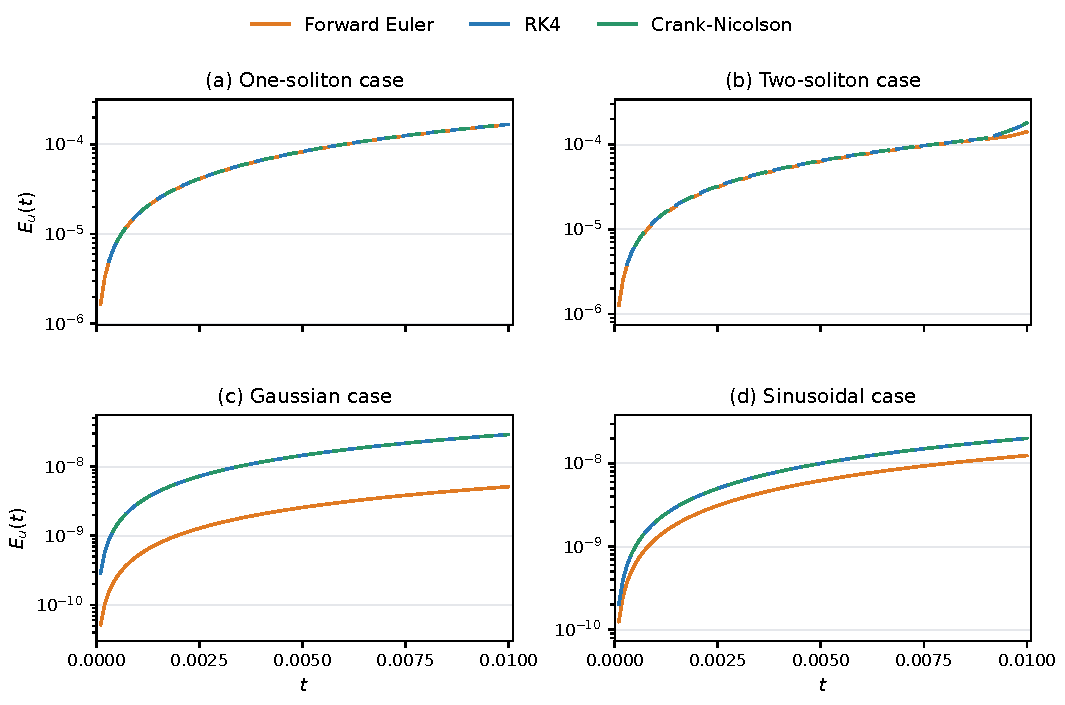
\includegraphics[width=\linewidth,trim=0 166.909bp 0 0,clip]{images/figure-09.pdf}\par
\noindent\begin{minipage}{\linewidth}
\noindent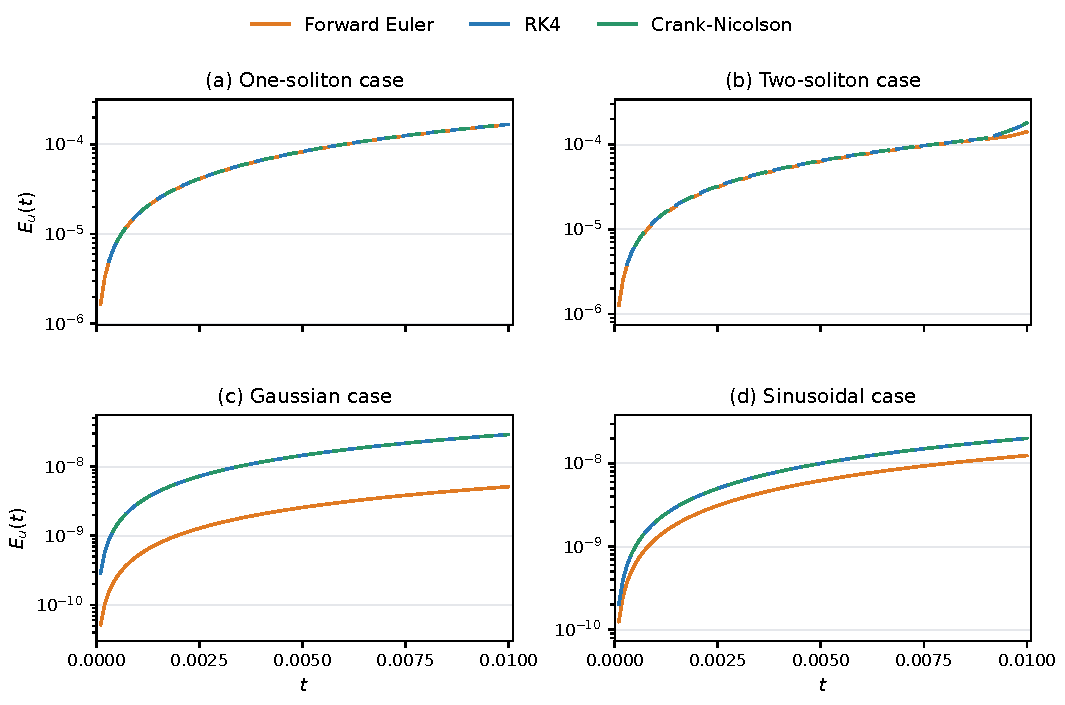
\includegraphics[width=\linewidth,trim=0 0 0 171.500bp,clip]{images/figure-09.pdf}\par
\captionof*{figure}{\textbf{Figure 9.} Development of the maximum absolute error in \(u\) for Centered-SD with forward Euler (orange), RK4 (blue) and Crank–Nicolson (green): (a) one-soliton, (b) two-soliton, (c) Gaussian and (d) sinusoidal cases. Each value is the maximum over the native field locations in the region of Section 5.1 and is evaluated at every time step; the vertical axis is logarithmic. All calculations use \(h=\Delta x=0.1\) and \(\Delta t=10^{-4}\). The initial error vanishes. Overlapping curves use alternating colors, with solid strokes where they separate.}
\end{minipage}


Figure 10 shows the corresponding histories for \(v\). The errors begin at zero and grow to their terminal values without numerical oscillations. RK4 and Crank–Nicolson remain close throughout the evolution. The forward Euler curve follows a similar shape above RK4, by factors of \(1.04\) and \(1.08\) in the two soliton tests and \(8.2\) and \(9.0\) in the Gaussian and sinusoidal tests.

\FloatBarrier
\noindent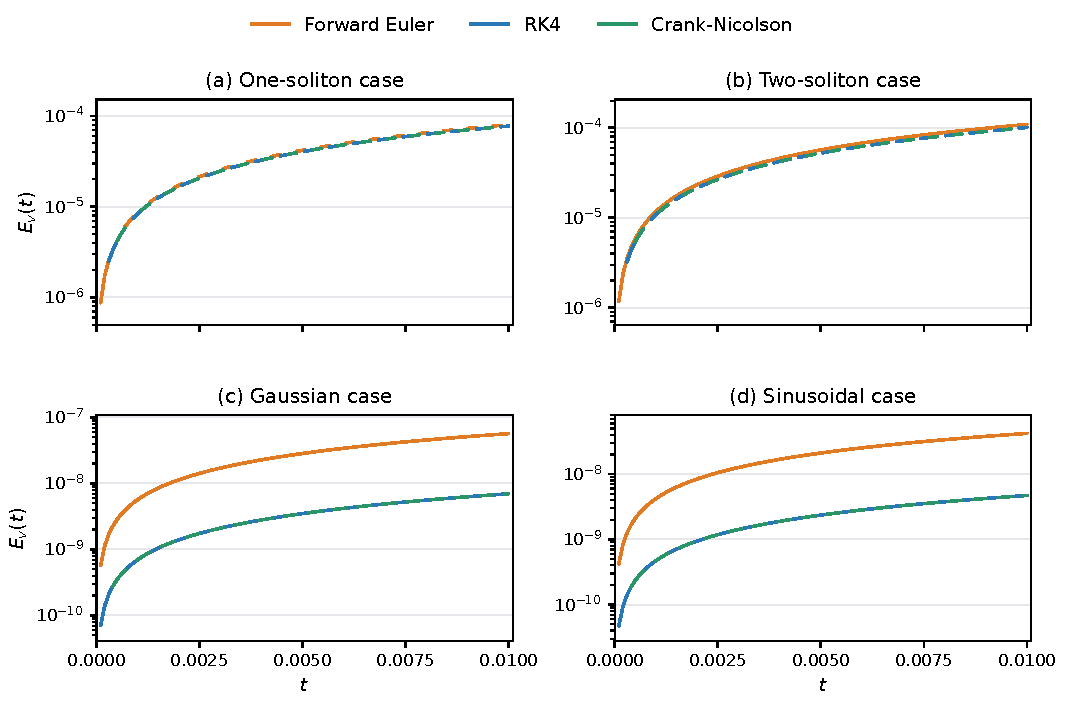
\includegraphics[width=\linewidth,trim=0 166.909bp 0 0,clip]{images/figure-10.pdf}\par
\noindent\begin{minipage}{\linewidth}
\noindent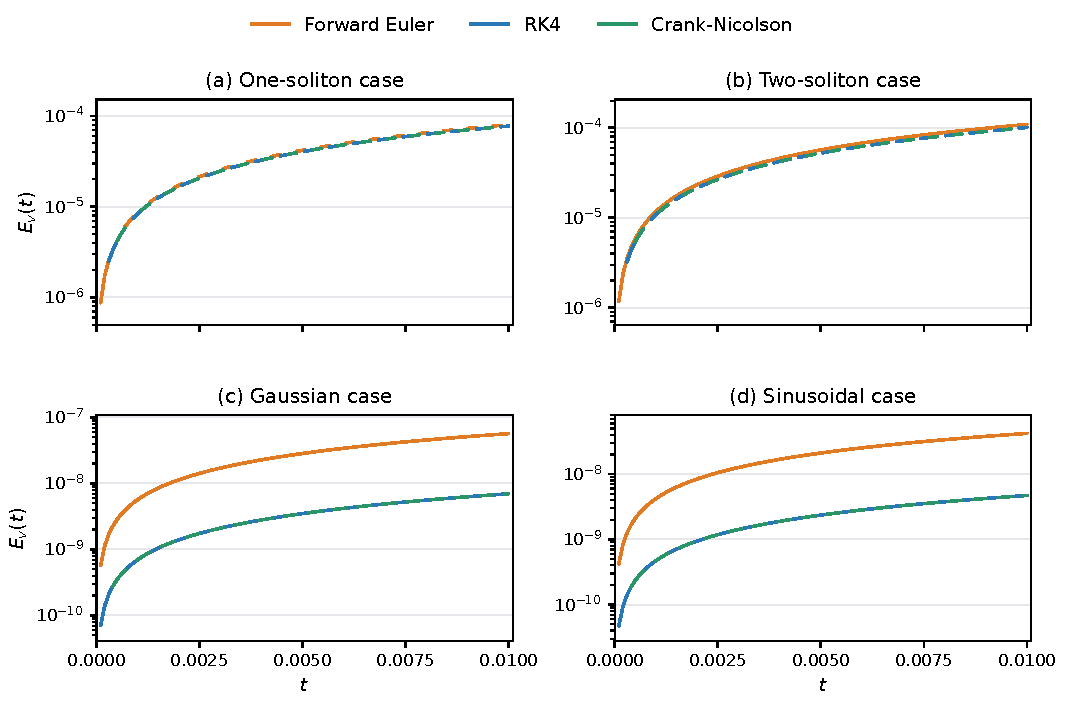
\includegraphics[width=\linewidth,trim=0 0 0 171.500bp,clip]{images/figure-10.pdf}\par
\captionof*{figure}{\textbf{Figure 10.} Development of the maximum absolute error in \(v\), with the same colors as Figure 9. Each value is the maximum over the native midpoints \(y_{k-1/2}\) of the second field in the region of Section 5.1. Overlapping curves use alternating colors, with solid strokes where they separate.}
\end{minipage}


The opposite shifts in the two field errors suggest that the temporal contribution partly cancels the spatial error in \(u\) and reinforces it in \(v\). To examine this interpretation, we halve the Euler time step to \(\Delta t=5\times10^{-5}\). The terminal error pair moves from \((1.664\times10^{-4},\,8.026\times10^{-5})\) to \((1.671\times10^{-4},\,7.880\times10^{-5})\) in the one-soliton test, and from \((1.420\times10^{-4},\,1.090\times10^{-4})\) to \((1.560\times10^{-4},\,1.048\times10^{-4})\) in the two-soliton test. In both cases, the errors move toward the RK4 values. This step-size response supports the cancellation and reinforcement interpretation and helps explain the smaller terminal \(u\) errors obtained with Euler at the tested step size.

The similar shapes of the error histories suggest that the spatial approximation and wave evolution largely determine the pattern of accumulation, while the time integrator changes its magnitude in each component. Read together with the spatial comparison, these results show why the initial derivative accuracy, the terminal field error and the response to a smaller time step describe different aspects of the same computation.

\FloatBarrier
\subsection*{5.4 Fixed and adaptive meshes}

In this subsection, we use the semi-discrete conservation law to examine how the distribution of spatial resolution affects the accuracy of Centered-SD. The soliton fields concentrate their variation along localized wave bands, and the conservation density provides a means of placing additional nodes in these regions. We compare uniform and adaptive meshes for the one- and two-soliton problems, following both the node distribution and the resulting physical-field errors. This allows us to examine how a conserved quantity from the semi-discrete system can guide the numerical resolution of its waves.

Both calculations use the same number of shared \(x\) nodes, the same uniform transverse lattice with \(h=0.1\), and RK4 with \(\Delta t=10^{-4}\) up to \(T=0.01\). The uniform \(x\) spacing is \(\Delta x=0.1\). On both meshes, the \(x\) derivatives are evaluated using the mapped three-point centered difference operators of Section 4.3, so that the comparison uses a common spatial approximation while varying the node distribution. The soliton backgrounds provide a positive transverse-averaged conservation density for the equidistribution construction.

In the adaptive runs, the initial \(x\) nodes are placed by equidistributing the transverse-averaged density \(\bar\rho\) computed from the exact initial fields, and the nodes subsequently evolve according to the conservation-based velocity of Section 4.3. The averaged density ranges from \(1.000\) in the background to \(1.150\) across the wave core in the one-soliton case, and from \(1.000\) to \(1.050\) in the wider domain of the two-soliton case. Figure 11 plots the resulting local grid spacing, normalized by the uniform spacing \(\Delta x=0.1\), at \(t=0\) and \(T=0.01\).

As seen in Figure 11, the equidistribution concentrates nodes in the region of larger density. In the one-soliton test, the local spacing contracts to \(0.90\Delta x\) across the wave trough while stretching to \(1.04\Delta x\) in the background; in the two-soliton test, it varies more mildly between \(0.97\Delta x\) and \(1.02\Delta x\). Over the short evolution to \(T=0.01\), the initial and final node distributions are nearly indistinguishable: the maximum node displacement is \(9.5\times10^{-4}\) in the one-soliton case and \(5.2\times10^{-4}\) in the two-soliton case, and the total discrete mass of \(\bar\rho\) is conserved to within \(10^{-7}\) relative error. The spatial resolution pattern is thus established by the initial equidistribution and adjusted only slightly by the node motion during the run.

\FloatBarrier
\begin{figure}[H]
\centering
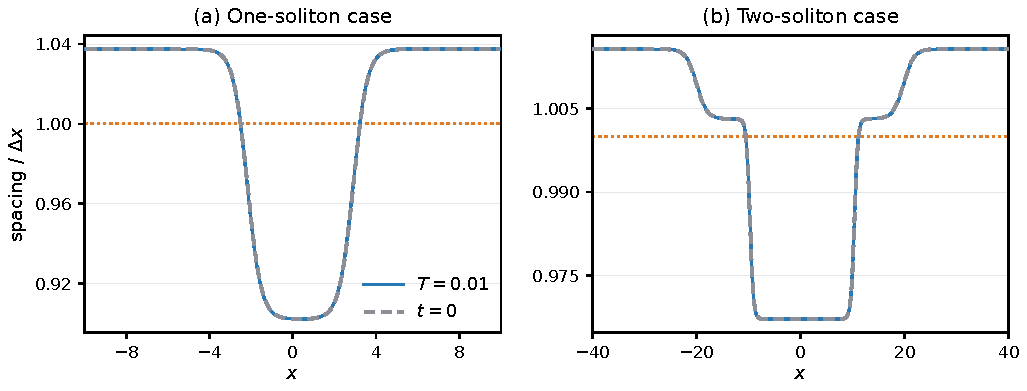
\includegraphics[width=.85\linewidth,height=.72\textheight,keepaspectratio]{images/figure-11.pdf}
\caption*{\textbf{Figure 11.} Local \(x\) spacing normalized by the uniform spacing \(\Delta x=0.1\), plotted at the interval midpoints of (a) the one-soliton and (b) the two-soliton case. Grey dashed: initial adaptive mesh; blue: \(T=0.01\); orange dotted: uniform spacing.}
\end{figure}



Table 5 compares the terminal errors at \(T=0.01\) on the uniform and adaptive meshes, measuring the relative improvement via

\paperdisplay{\mathcal R_f=100\left(1-\frac{E_f^{\mathrm{adaptive}}(T)}{E_f^{\mathrm{uniform}}(T)}\right)\%,\qquad f=u,v.}{\tag{132}}
 
\begin{table}[!htbp]
\centering
\caption*{Table 5. Physical-field errors at T = 0.01 on the uniform and adaptive meshes, with the relative change defined in the text. Both calculations use Centered-SD with mapped centred x differences, RK4, \(\Delta\)t = 10\textsuperscript{-}\textsuperscript{4} and the same number of nodes.}
\small
\setlength{\tabcolsep}{4pt}
\renewcommand{\arraystretch}{1.22}
\begin{tabularx}{\linewidth}{YYYYYYY}
\toprule
Case & \multicolumn{2}{>{\raggedright\arraybackslash}p{2\dimexpr\linewidth/7-2\tabcolsep\relax}}{Uniform mesh} & \multicolumn{2}{>{\raggedright\arraybackslash}p{2\dimexpr\linewidth/7-2\tabcolsep\relax}}{Adaptive mesh} & \multicolumn{2}{>{\raggedright\arraybackslash}p{2\dimexpr\linewidth/7-2\tabcolsep\relax}}{Change} \\
 & \(E_u\) & \(E_v\) & \(E_u\) & \(E_v\) & \(\mathcal R_u\) & \(\mathcal R_v\) \\
\midrule
One-soliton & 6.741 \(\times\) 10\textsuperscript{-4} & 1.401 \(\times\) 10\textsuperscript{-3} & \textbf{5.954 \(\times\) 10\textsuperscript{-4}} & \textbf{1.157 \(\times\) 10\textsuperscript{-3}} & 11.7\% & 17.4\% \\
Two-soliton & 5.533 \(\times\) 10\textsuperscript{-4} & 1.589 \(\times\) 10\textsuperscript{-3} & \textbf{5.198 \(\times\) 10\textsuperscript{-4}} & \textbf{1.501 \(\times\) 10\textsuperscript{-3}} & 6.0\% & 5.6\% \\
\bottomrule
\end{tabularx}
\end{table}

Positive values of \(\mathcal R_f\) indicate an error reduction. The adaptive mesh lowers the errors in both physical fields for both test problems: by \(11.7\%\) in \(u\) and \(17.4\%\) in \(v\) for the one-soliton case, and by \(6.0\%\) in \(u\) and \(5.6\%\) in \(v\) for the two-soliton case. These improvements are modest and commensurate with the \(3\%\)–\(10\%\) local spacing reductions shown in Figure 11, but they occur consistently across both components without degrading either field. Moreover, a control calculation in which the initially equidistributed nodes are held fixed in time (\(\mathcal V_i=0\)) yields reductions of \(12.8\%\) and \(16.3\%\) for the one-soliton case and \(5.3\%\) and \(5.8\%\) for the two-soliton case — within \(1.1\) percentage points of the moving-mesh values in Table 5. Over this short time interval, the accuracy gain therefore comes primarily from the initial density-adapted node placement rather than from dynamic node motion.

To show where this reduction takes place in space, Figure 12 plots the transverse-maximum error profiles \(\max_{|y|<5}|u_h-u^*|\) and \(\max_{|y|<5}|v_h-v^*|\) as functions of \(x\) for the one-soliton case. On the uniform mesh, the numerical error is not distributed evenly across the domain, but is localized along the central wave band \(x\in[-3,3]\). Because the conservation density \(\bar\rho\) peaks in this same band, the equidistribution shifts nodes from the quiet background directly into the region where the truncation error is generated. As a result, the adaptive mesh lowers the maximum errors and the main error peaks — reducing the main peak in \(u\) from \(6.74\times10^{-4}\) to \(5.95\times10^{-4}\) and lowering the broad plateau in \(v\) from \(1.40\times10^{-3}\) to \(1.16\times10^{-3}\). We also notice that the relative gain in the one-soliton test is larger for \(v\) (\(17.4\%\)) than for \(u\) (\(11.7\%\)). This is natural in the Centered-SD formulation: the monitor density \(\rho_k=1-\omega_k/h\) is a shifted rescaling of the auxiliary variable \(\omega_k\), which enters the staggered reconstruction \(v_k=\Delta_hu_k+\frac2h(\omega_k+\omega_{k-1})\) and specifically weights the part of \(v\) not captured by the backward difference of \(u\).

\FloatBarrier
\begin{figure}[H]
\centering
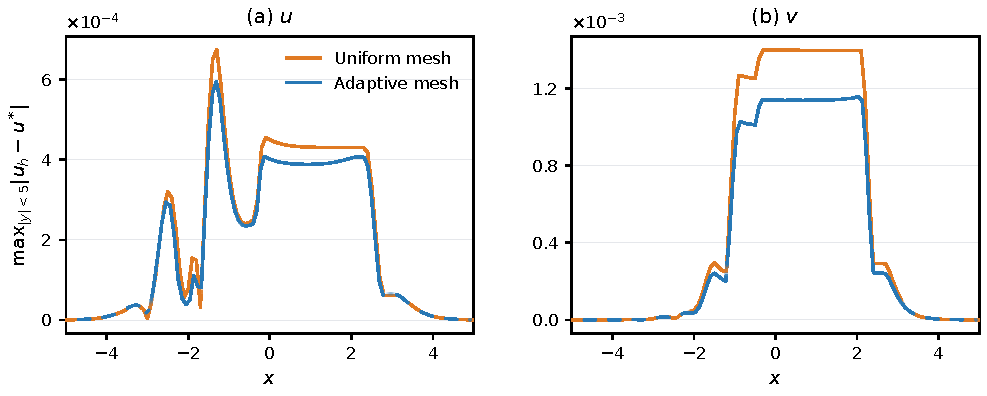
\includegraphics[width=.85\linewidth,height=.72\textheight,keepaspectratio]{images/figure-12.pdf}
\caption*{\textbf{Figure 12.} One-soliton case at \(T=0.01\). Maximum over the transverse layers of the absolute error at each native \(x\) node for the uniform mesh (orange) and the adaptive mesh (blue): (a) \(u\) and (b) \(v\). Both calculations use the mapped centred operators of Section 4.3, the same number of nodes and RK4 with \(\Delta t=10^{-4}\).}
\end{figure}

The mesh experiments show that the semi-discrete conservation density provides a useful basis for allocating spatial resolution. Equidistribution concentrates nodes along the soliton wave bands, where the uniform-grid errors are also largest, and reduces the errors in both physical fields at the same node count. The spatial error profiles further show that this improvement extends across the wave region, connecting the change in node placement with the location of the computed errors.

Over the present time interval, the node distribution changes only slightly, and the calculation with a fixed, initially adapted mesh gives similar error reductions. The main benefit therefore comes from the resolution pattern established by the conservation density. These results give the conservation law a concrete role in numerical computation: it guides the placement of nodes in a way that improves the approximation of the physical fields. The mesh construction thus provides a further connection between the analytical structure of the semi-discrete system and the accurate computation of its waves.

\FloatBarrier
\subsection*{5.5 Evolution of independent physical-field perturbations}

The preceding experiments start from prescribed reference wave fields and examine how accurately their evolution is reproduced. A related question concerns the response of the numerical evolution when the initial physical fields are slightly changed. Such changes may arise when initial data are sampled or prescribed, and their influence develops through the coupling between the two fields. A disturbance introduced into \(u\) can generate a response in \(v\), while a disturbance in \(v\) can also affect the subsequent evolution of \(u\). Understanding this response helps describe how the computed waves depend on their initial physical data.

We examine this dependence on the same four backgrounds by perturbing \(u_0\) and \(v_0\) separately. For each spatial formulation, the perturbed evolution is measured relative to its own unperturbed trajectory. This separates the continuing response in the initially disturbed field from the response generated in the other component, allowing us to follow both processes over time. The two experiments add \(\varepsilon\Phi\) to \(u_0\) or \(v_0\), respectively, with

\paperdisplay{\Phi(x,y)=\sin^2\!\left(\frac{\pi(y-y_L)}{y_R-y_L}\right)\cos(\kappa x),\qquad \varepsilon=10^{-6},\qquad \kappa=\frac{\pi}{2}.}{\tag{133}}

The perturbation is sampled at each field's native sites. The transverse node intervals are \([-9.95,9.95]\) for the one-soliton case, \([-39.95,39.95]\) for the two-soliton case, and \([-2,2]\) for the Gaussian and sinusoidal cases. The envelope and its first derivative vanish at the transverse endpoints. All trajectories use \(h=\Delta x=0.1\), RK4, \(\Delta t=10^{-4}\), and \(T=0.01\), with the prescribed lower \(u\) trace and the boundary closures of Section 4.2.

For each spatial formulation, let \((u_h^\varepsilon,v_h^\varepsilon)\) and \((u_h^0,v_h^0)\) be its perturbed and unperturbed numerical trajectories. We record \(\delta u_h=u_h^\varepsilon-u_h^0\) and \(\delta v_h=v_h^\varepsilon-v_h^0\), and plot their native-node maximum magnitudes divided by \(\varepsilon\) in the observation regions of Section 5.1. The initial ordinates are the maxima of the imposed perturbation sampled at those same sites. The nonlinear difference equations are advanced together with the corresponding background at every RK4 stage.

For the one-soliton background, Figure 13 follows both perturbation directions. With \(u_0\) perturbed, the response in \(u\) remains near its initial amplitude and grows slightly, while the initially unperturbed \(v\) field develops a response from zero. For Endpoint-SD, Centered-SD, and FD, the terminal induced \(v\) responses are \(0.09182\), \(0.09186\), and \(0.09185\) times \(\varepsilon\), respectively. With \(v_0\) perturbed, each formulation produces a growing \(u\) response reaching approximately \(0.225\varepsilon\), alongside a small increase in the initially imposed \(v\) disturbance. The two inputs thus expose both the persistence of the original disturbance and the response generated through coupling.

\FloatBarrier
\noindent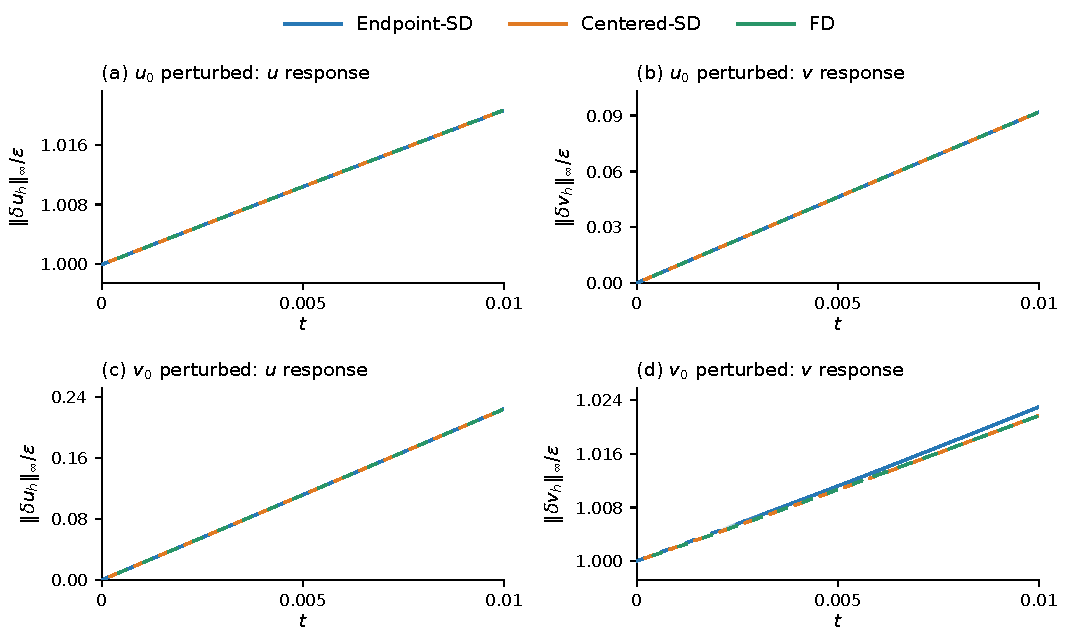
\includegraphics[width=\linewidth,trim=0 141.893bp 0 0,clip]{images/figure-13.pdf}\par
\noindent\begin{minipage}{\linewidth}
\noindent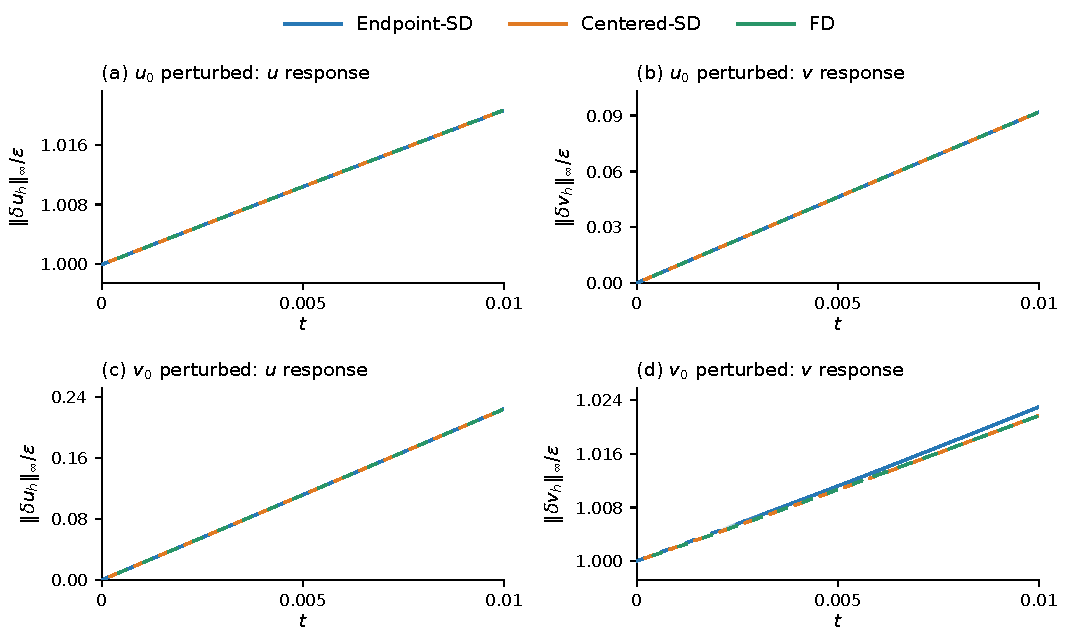
\includegraphics[width=\linewidth,trim=0 0 0 166.000bp,clip]{images/figure-13.pdf}\par
\captionof*{figure}{Figure 13. One-soliton perturbation responses. The upper and lower rows perturb \(u_0\) and \(v_0\), respectively; the columns show the normalized \(u\) and \(v\) responses. Blue: Endpoint-SD; orange: Centered-SD; green: FD. Each curve uses its own unperturbed trajectory and native field sites. Where curves overlap, their colors alternate; separated curves are solid. The Endpoint-SD response in panel (d) is slightly larger than the other two responses.}
\end{minipage}


The two-soliton background produces a substantial induced \(u\) response when the initial perturbation is applied to \(v_0\) (Figure 14). By \(T=0.01\), this response reaches approximately \(0.974\varepsilon\) within each formulation, while the \(v\) response remains close to its initial magnitude. For the reverse input, an initial \(u_0\) perturbation produces terminal \(v\) responses of \(0.10280\varepsilon\), \(0.10278\varepsilon\), and \(0.10277\varepsilon\) for Endpoint-SD, Centered-SD, and FD, respectively. These histories show how a disturbance initially confined to one component develops into a response in both physical fields on the interacting-wave background.

\FloatBarrier
\noindent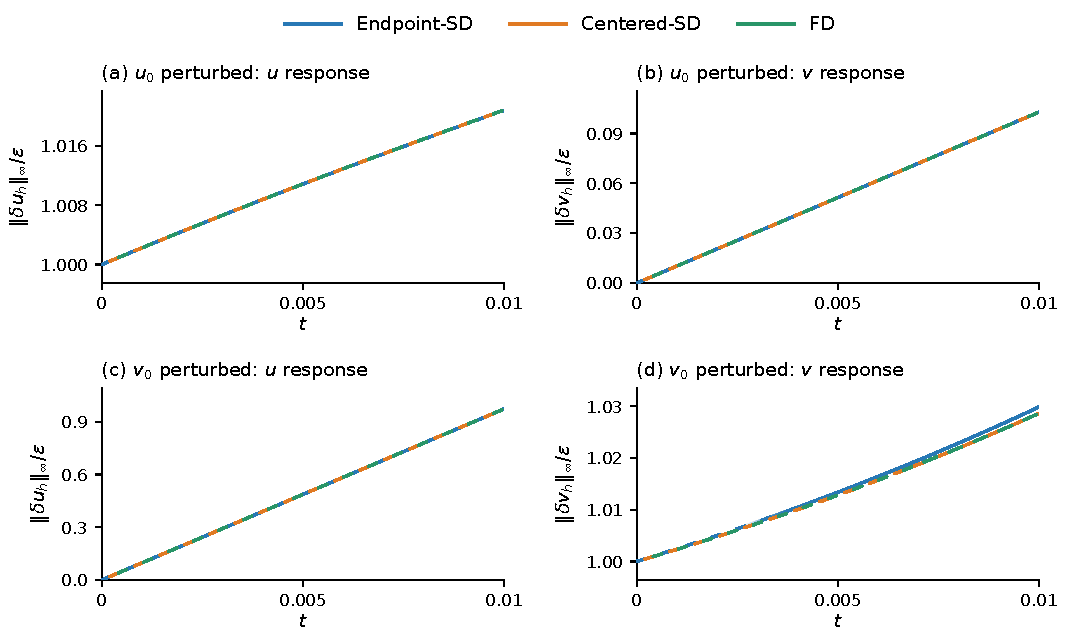
\includegraphics[width=\linewidth,trim=0 141.893bp 0 0,clip]{images/figure-14.pdf}\par
\noindent\begin{minipage}{\linewidth}
\noindent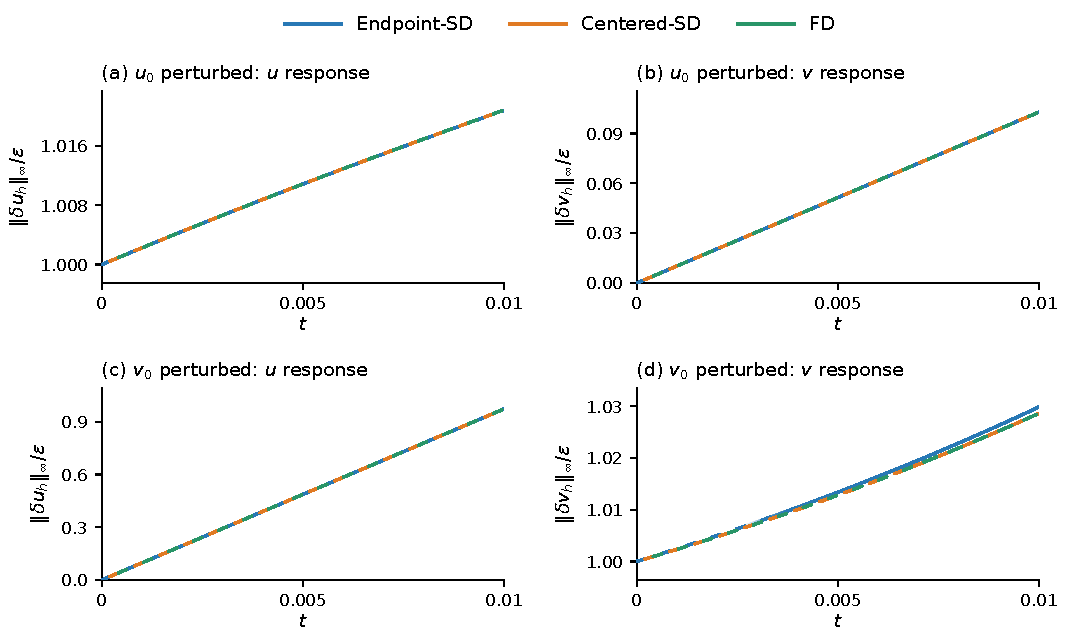
\includegraphics[width=\linewidth,trim=0 0 0 166.000bp,clip]{images/figure-14.pdf}\par
\captionof*{figure}{Figure 14. Two-soliton perturbation responses. The upper and lower rows perturb \(u_0\) and \(v_0\), respectively; the columns show the normalized \(u\) and \(v\) responses. Blue: Endpoint-SD; orange: Centered-SD; green: FD. Each curve uses its own unperturbed trajectory and native field sites. Where curves overlap, their colors alternate; separated curves are solid. The Endpoint-SD response in panel (d) is slightly larger than the other two responses.}
\end{minipage}


On the Gaussian and sinusoidal backgrounds, the initially perturbed component stays close to its initial magnitude over the computed interval, while a smaller response develops in the other field. Table 6 records the terminal responses separately for each formulation. An initial \(u_0\) disturbance induces a \(v\) response of approximately \(0.019\varepsilon\), and a \(v_0\) disturbance induces a \(u\) response of approximately \(0.049\varepsilon\). The full time histories are included in the supplementary response plots.

\begin{table}[!htbp]
\centering
\caption*{Table 6. Terminal normalized responses on the Gaussian and sinusoidal backgrounds at \(T=0.01\). Each pair gives \((\|\delta u_h\|_\infty/\varepsilon,\|\delta v_h\|_\infty/\varepsilon)\) for the indicated initial perturbation.}
\small
\setlength{\tabcolsep}{4pt}
\renewcommand{\arraystretch}{1.22}
\begin{tabularx}{\linewidth}{YYYY}
\toprule
Method & Background & \(u_0\) perturbed & \(v_0\) perturbed \\
\midrule
Endpoint-SD & Gaussian & (0.99837, 0.01935) & (0.04922, 0.99684) \\
 & Sinusoidal & (0.99841, 0.01933) & (0.04922, 0.99687) \\
Centered-SD & Gaussian & (0.99837, 0.01935) & (0.04922, 0.99683) \\
 & Sinusoidal & (0.99841, 0.01933) & (0.04922, 0.99687) \\
FD & Gaussian & (0.99837, 0.01935) & (0.04921, 0.99837) \\
 & Sinusoidal & (0.99841, 0.01933) & (0.04922, 0.99841) \\
\bottomrule
\end{tabularx}
\end{table}

These experiments show how a small change in one initial physical field develops through the coupled numerical evolution. Within each formulation, the initially perturbed component remains close to its original disturbance magnitude over the computed interval, while the other field acquires a response whose magnitude depends on the background and the perturbed component. The substantial induced \(u\) response in the two-soliton case is consistent with the transverse integration in the first field equation, through which the influence of a \(v\) perturbation can accumulate across the domain. Following the two inputs separately therefore helps us understand both the persistence of an initial disturbance and the response generated by the coupling. Alongside the preceding accuracy tests, these histories describe how the computed waves respond to changes in their physical initial data.

\FloatBarrier
\section*{6. Conclusions}

In this work, building on the bilinear formulation and exact solutions of the continuous DLW system, we have developed two related integrable semi-discretizations. A Miwa expansion of the Hirota–Miwa equation gives Endpoint-SD, from which we obtain Centered-SD through a half-step parameter shift and a staggered placement of the \(\tau\) functions. For both formulations, we construct explicit Gram determinant solutions, establish common positivity conditions for regular field reconstruction, and derive Darboux–Lax representations compatible with the nonlinear equations. These shared structures allow us to examine how lattice placement affects the approximation of the physical waves.

We then examine the continuum limits of the equations and exact wave fields to make this dependence explicit. Endpoint-SD is second-order consistent in the first physical-field equation and first-order consistent in the second, whereas Centered-SD is second-order consistent in both. For Endpoint-SD, we identify the leading residual correction associated with its endpoint arrangement. For Centered-SD, matching the Gram solutions to the continuous family establishes second-order approximation of both exact physical fields under the stated regularity and positivity assumptions. The comparison thus traces the effect of lattice placement through the reconstructed equations and, for Centered-SD, through the wave profiles themselves.

Through numerical experiments, we follow these approximation properties from the initial time derivatives to the evolved physical fields. Endpoint-SD gives the smallest initial \(u_t\) error in all four tests and retains the smallest terminal \(u\) error on the Gaussian and sinusoidal backgrounds. In the soliton tests, Centered-SD gives smaller terminal errors in both fields than Endpoint-SD, illustrating the importance of assessing the two components through their coupled evolution. Keeping the spatial formulation fixed, we further examine how time integration modifies these errors. The Euler step-size controls support partial cancellation of spatial and temporal errors in \(u\) and reinforcement in \(v\), showing how their combined effect depends on the physical-field component.

We also use the semi-discrete conservation law to guide the allocation of spatial resolution. Its density concentrates shared longitudinal nodes along the soliton wave bands and improves both field errors at a fixed node count. Over the computed interval, the gain comes mainly from the initial density-adapted placement, demonstrating the usefulness of this quantity for mesh design. To complement these accuracy comparisons, we perturb the initial fields independently and follow both the persistence of the imposed disturbance and the response generated in the other component.

The DLW construction therefore connects a choice made at the bilinear lattice level to the approximation and computation of the physical waves. Exact solutions support the continuum comparison, while the conservation density guides the allocation of spatial resolution. In this way, the integrable structure provides a foundation for understanding and improving the approximation of continuous waves through the design of their discrete representations.

\FloatBarrier
\section*{Appendix A. Determinant identities and alternative solution representations}

Every field used in the main text is a logarithmic derivative of a \(\tau\) function, so its evaluation reduces to an identity for a determinant and for the derivatives of that determinant. This appendix records the three identities on which the reconstruction rests, together with the relation between the two determinant families and the explicit low-order members.

\textbf{Rank-one identity.} Let \(M(\theta)=M_0+\theta\,r\,c^{\mathsf T}\) with \(M_0\) invertible and \(r,c\) column vectors. Factoring \(M_0\) out of the rows of \(M(\theta)\) gives

\paperdisplay{\det M(\theta)=\det M_0\left(1+\theta\,c^{\mathsf T}M_0^{-1}r\right),\qquad \partial_\theta\log\det M(\theta)=c^{\mathsf T}M^{-1}r .}{\tag{A1}}

The second form follows from the first together with the Sherman–Morrison formula for \(M^{-1}\), and it is the only identity needed to differentiate a determinant in a parameter that enters linearly.

\textbf{Shift identity.} The two families (46) and (51) differ only in their phases. Writing \(\xi_i+\eta_j=(z_i+w_j)[x-2at+(w_j-z_i)t]\) for the Endpoint family, the additional factor \(e^{-h(z_i+w_j)t}\) in (51) replaces \(a\) by \(a+h/2\) in the same exponent. Hence

\paperdisplay{\tau_n^{\mathrm C}(k;h)=\tau_n^{\mathrm E}(k;h)\big|_{a\to a+h/2},}{\tag{A2}}

so the two determinant families share their minors and their positivity, and only the reference value of the bilinear parameter changes. This is the determinant counterpart of the shift introduced in Section 2.3, and it is why the centered pairings carry \(a\pm h/2\).

\textbf{Logarithmic fields.} With \(f_k=\tau_0(k)\) and \(g_k=\tau_1(k)\) the definitions (57) and (71) become ratios of neighbouring determinants,

\paperdisplay{U_k=2\partial_x\log\frac{\tau_0(k)}{\tau_1(k)},\qquad V_k=\frac2h\partial_x\log\frac{\tau_0(k)\tau_1(k)}{\tau_0(k-1)\tau_1(k-1)},}{\tag{A3}}

and analogously for \(u_k\), \(v_k\) through (71). Smoothness of the fields is therefore equivalent to positivity of the \(\tau\) functions, which Proposition 2.3 guarantees on the class (53). The same argument applies to the derivatives: since the phase factors are positive on that class, every principal minor of \(M-C\) keeps the sign of the corresponding Cauchy minor (54), and the cofactor identity \(\det M\,(M^{-1})_{ij}=\mathrm{cof}_{ji}M\) shows that the first minors inherit this sign. The reconstructed fields and their \(x\) derivatives are consequently bounded on the region away from the lattice boundary.

\textbf{Low-order members.} For \(N=1\) with \(c_{11}=1\), writing \(A=\alpha\beta/(z+w)\) gives \(\tau_n(k)=1+A(-w/z)^nL(h)^k e^{\xi+\eta}\). Substitution into (A3) reproduces the standard one-soliton field at the node and edge locations, and the two-soliton case used in Section 5 is the same formula with a \(2\times2\) Cauchy matrix. The family with \(c_{ij}=\delta_{ij}\) is the Gram reduction of the usual Casoratian determinants of the hierarchy [15]; we use the Gram form throughout because the Miwa expansion acts on it directly.

\FloatBarrier
\section*{Appendix B. Field transformations and reconstruction conditions}

The numerical state of Centered-SD is the pair \((u_k,\omega_k)\), whereas the physical comparison is made in the fields \((u,v)\). This appendix records the two transformations between them, the conditions under which they are equivalent, and the lower trace required by the computation.

\textbf{Field relation and recurrence.} The definitions (71) imply, for every edge,

\paperdisplay{v_k-\Delta_hu_k=\frac2h\left(\omega_k+\omega_{k-1}\right),\qquad \omega_k=\partial_x\log\frac{g_k}{g_{k-1}},}{\tag{B1}}

where the second expression shows that \(\omega_k\) is the lattice difference of the logarithmic potential and therefore carries a factor \(h\) relative to \(v-u_y\). Rearranging (B1) gives the reconstruction (72),

\paperdisplay{\omega_0=b,\qquad \omega_k=\frac h2\left(v_k-\Delta_hu_k\right)-\omega_{k-1},\qquad k=1,\dots,N .}{\tag{B2}}

The recurrence is linear and lower triangular, so it determines \((\omega_1,\dots,\omega_N)\) uniquely from the physical fields and the single lower value \(b\). Its solution is

\paperdisplay{\omega_k=(-1)^k b+\frac h2\sum_{j=1}^{k}(-1)^{k-j}\left(v_j-\Delta_hu_j\right),}{\tag{B3}}

in which the coefficients have modulus one. An error in the lower trace alone propagates with alternating sign and unchanged magnitude, while errors in the edge differences can accumulate through the sum. The reconstruction is an exact affine relation and requires no branch selection.

\textbf{Conditions on the lower trace.} For the \(\tau\) functions of Theorem 2.1 the compatible trace is fixed by the lattice, namely \(b=\partial_x\log(g_0/g_{-1})\). In a computation the data are prescribed in the physical fields, so the trace is taken instead from the continuous reference, \(\omega_0=h(v^*-u_y^*)/4\) evaluated at the lower node. The two agree to \(O(h^2)\) on the smooth class of Section 3.4, and the resulting discrepancy enters (B3) with alternating sign only, that is without growth along the layer index. During the evolution the lower value is advanced by the same equation as the interior, so the trace is not frozen.

\textbf{Consistency of the initial data.} Equation (B2) reproduces \(v_k\) on every edge by construction. Once the lower trace is supplied, \((u,\omega)\) represents the prescribed physical fields \((u,v)\). Changing the lower trace by \(\delta b\) and repeating the recurrence adds \(\delta\omega_k=(-1)^k\delta b\). Its adjacent values sum to zero, so the reconstructed initial \(v_k\) remains unchanged. This alternating auxiliary component can affect the subsequent evolution; the lower trace is therefore specified together with the physical initial data. All computations in Section 5 use the construction above.

\FloatBarrier
\section*{Appendix C. Operator compatibility and continuum expansions}

Two computations are compressed in the main text: the reduction of the compatibility condition (88) to scalar coefficient relations, and the expansions that yield the residuals (110), (111) and (113). We record both.

\textbf{Coefficient form of the compatibility condition.} Expanding \(L_t+LM-\widetilde ML\) with the rules \(Dq=qD+q_x\) and \(Yq_k=q_{k-1}Y\) produces terms proportional to \(DY\), \(Y\), \(D\) and \(D^0\). The coefficients of \(DY\), \(Y\) and \(D^0\) vanish by (94), (97) and (99), respectively, and the coefficient of \(D\) vanishes identically. Since \(L\) and \(M\) are at most second order in \(D\), the compatibility condition (88) is therefore equivalent to those three scalar relations.

\textbf{Midpoint expansions.} For smooth \(q\) sampled at the nodes and edges of the lattice,

\paperdisplay{\Delta_hq_k=q_y+\frac{h^2}{24}q_{yyy}+O(h^4),\qquad \mathcal M_-q_k=q+\frac{h^2}{8}q_{yy}+O(h^4),}{\tag{C1}}

evaluated at the edge midpoint. Substituting (C1) into the first Endpoint-SD equation gives \(\mathcal R_u+O(h^2)\), since both the difference and the average are second-order accurate there. The second equation carries an additional term from the flux. Expanding its bracket at the midpoint gives

\paperdisplay{(u+2a)v-4u+u_{xy}+\frac h4\left(v^2-u_y^2-8v\right)+O(h^2),}{\tag{C2}}

and applying \(\partial_x\) produces the coefficient \(\tfrac h4\partial_x(v^2-u_y^2-8v)\) recorded in (110).

\textbf{Centered reconstruction.} The relation \(v_k=\Delta_hu_k+\mathcal M_-W_k\) with \(W_k=4\omega_k/h\) expands as

\paperdisplay{v=u_y+W+h^2\left(\frac{u_{yyy}}{24}+\frac{W_{yy}}8\right)+O(h^4),}{\tag{C3}}

so on the smooth family with \(W=v-u_y+O(h^2)\) the reconstructed second field is second-order accurate. The extra flux of the first equation is \(\omega^2/2-h\omega=h^2(W^2/32-W/4)\), whose lattice difference and subsequent \(x\) derivative are \(O(h^2)\), so the first residual is again \(\mathcal R_u+O(h^2)\). Differentiating (C3) in time and using \(W_t=W_{xx}-\partial_x[(u+2a)W-4u]\) from (77) shows that the second residual is \(\mathcal R_v+O(h^2)\), which is the content of (111).

\FloatBarrier
\section*{Appendix D. Numerical implementation and supplementary experiments}

This appendix collects the conventions of the computations, the closures at the transverse ends, and the control runs quoted in Sections 5.3 and 5.4.

\textbf{\(x\) derivatives.} All formulations use the same periodic Fourier operators, with multipliers \(\mathrm i\xi\) for \(\mathcal D_x\) and \(-\xi^2\) for \(\mathcal D_{xx}\). The first-derivative multiplier is set to zero at the Nyquist frequency, the second retains its value there, and products are evaluated pointwise. No filtering, dealiasing or artificial viscosity is applied in any run.

\textbf{Closures.} Endpoint-SD advances \((u_k,v_k)\) with the prescribed lower value of \(u_t\) and a backward chain, so no upper datum is required. FD uses the same lower data and, at the upper end, the rule \(u_{N+1}=u^*_{N+1}+3e_N-3e_{N-1}+e_{N-2}\) with \(e_k=u_k-u^*_k\), together with its differentiated form when \(\dot u\) is needed. Centered-SD advances \((u_k,\omega_k)\), needs no upper ghost, and advances the lower \(\omega\) trace by the same equation as the interior.

\textbf{Implicit step.} Crank–Nicolson is solved by an Euler predictor followed by fixed-point iteration on the trapezoidal residual. The implementation advances \((u,w)\), where \(w=4\omega/h\). In the notation of the field equations, the trapezoidal residual satisfies \(\max\{\|r_u\|_\infty,(4/h)\|r_\omega\|_\infty\}<2\times10^{-14}\) at termination. A control calculation with a stopping level of \(2\times10^{-15}\) changes the terminal error norms of Section 5.3 by at most \(8\times10^{-10}\).

\textbf{Moving mesh.} On a nonuniform mesh the derivatives are mapped to the fixed computational coordinate, with \(D_xf=\partial_\xi f/J\) and \(D_{xx}f=\partial_{\xi\xi}f/J^2-(\partial_\xi J)(\partial_\xi f)/J^3\), where \(J=1+\partial_\xi s\) and \(x_i=\xi_i+s_i\). The three-point formulas of Section 4.3 evaluate \(\partial_\xi\) and \(\partial_{\xi\xi}\) on the uniform computational grid, and the node motion is coupled to the field equations through \(\dot z=F_z+\mathcal V D_xz\). The uniform-mesh results of Table 5 use the same operators with \(s=0\) and \(\mathcal V=0\).

The control runs underlying Sections 5.3 and 5.4 are summarized below. They use the same Centered-SD state, grid and reference as the corresponding main runs, and a single quantity is changed in each row.

\begin{table}[!htbp]
\centering
\caption*{Table 7. Control runs for Section 5. The change column states the only difference from the corresponding main run.}
\small
\setlength{\tabcolsep}{4pt}
\renewcommand{\arraystretch}{1.22}
\begin{tabularx}{\linewidth}{YYYY}
\toprule
Run & Change & \(E_u\) & \(E_v\) \\
\midrule
One soliton\newline Euler & main, \(\Delta t=10^{-4}\) & \(1.664\times10^{-4}\) & \(8.026\times10^{-5}\) \\
 & half step, \(\Delta t=5\times10^{-5}\) & \(1.671\times10^{-4}\) & \(7.880\times10^{-5}\) \\
Two solitons\newline Euler & main, \(\Delta t=10^{-4}\) & \(1.420\times10^{-4}\) & \(1.090\times10^{-4}\) \\
 & half step, \(\Delta t=5\times10^{-5}\) & \(1.560\times10^{-4}\) & \(1.048\times10^{-4}\) \\
All, CN & tight solve, \(2\times10^{-15}\) & terminal error norms change by at most \(8\times10^{-10}\) \\
Mesh\newline one soliton & adaptive, nodes moving & \(5.954\times10^{-4}\) & \(1.157\times10^{-3}\) \\
 & equidistributed, frozen & \multicolumn{2}{>{\raggedright\arraybackslash}p{2\dimexpr\linewidth/4-2\tabcolsep\relax}}{reductions of \(12.8\%\) and \(16.3\%\) relative to the uniform mesh} \\
\bottomrule
\end{tabularx}
\end{table}

The half-step rows show that the first-order temporal defect of forward Euler accounts for the whole displacement of its error level, as discussed in Section 5.3. The tight-solve row shows that the terminal error norms change by less than the reported discrepancies between integrators when the stopping tolerance is reduced. The frozen row separates the two parts of the mesh construction: with the node count fixed, most of the reduction in Table 5 is already obtained by the initial equidistribution, as stated in Section 5.4.

\subsubsection*{Resolving the RK4 and Crank–Nicolson differences}

Table 8 resolves the entries that coincide after rounding in Table 4. It lists twelve significant digits from the saved terminal error norms and their signed difference, C–N minus RK4. A positive difference means that RK4 has the smaller recorded error. Both methods advance the same spatial system with a small time step, so their total physical-field errors are close even though their temporal approximations differ. The extra digits resolve this difference at the parameters used in the main experiment.

\begin{table}[!htbp]
\centering
\caption*{Table 8. Terminal RK4 and Crank–Nicolson error norms at T = 0.01, with h = \(\Delta\)x = 0.1 and \(\Delta\)t = 10\textsuperscript{-}\textsuperscript{4}. The last column compares the two saved main runs.}
\small
\setlength{\tabcolsep}{4pt}
\renewcommand{\arraystretch}{1.22}
\begin{adjustbox}{max width=\linewidth}
\begin{tabular}{llrrrl}
\toprule
Case & Field & RK4 & Crank–Nicolson & C–N - RK4 & Smaller error \\
\midrule
One-soliton & \textit{u} & 1.67723337656 \(\times\) 10\textsuperscript{-4} & 1.67723193356 \(\times\) 10\textsuperscript{-4} & -1.44300 \(\times\) 10\textsuperscript{-10} & C–N \\
 & \textit{v} & 7.73375836247 \(\times\) 10\textsuperscript{-5} & 7.73376020056 \(\times\) 10\textsuperscript{-5} & 1.83809 \(\times\) 10\textsuperscript{-11} & RK4 \\
Two-soliton & \textit{u} & 1.79163370095 \(\times\) 10\textsuperscript{-4} & 1.80474053431 \(\times\) 10\textsuperscript{-4} & 1.31068 \(\times\) 10\textsuperscript{-6} & RK4 \\
 & \textit{v} & 1.00906108654 \(\times\) 10\textsuperscript{-4} & 1.00948746633 \(\times\) 10\textsuperscript{-4} & 4.26380 \(\times\) 10\textsuperscript{-8} & RK4 \\
Gaussian & \textit{u} & 2.89993671090 \(\times\) 10\textsuperscript{-8} & 2.89992077157 \(\times\) 10\textsuperscript{-8} & -1.59393 \(\times\) 10\textsuperscript{-13} & C–N \\
 & \textit{v} & 6.96696389468 \(\times\) 10\textsuperscript{-9} & 6.96879887130 \(\times\) 10\textsuperscript{-9} & 1.83498 \(\times\) 10\textsuperscript{-12} & RK4 \\
Sinusoidal & \textit{u} & 2.00293429689 \(\times\) 10\textsuperscript{-8} & 2.00290237694 \(\times\) 10\textsuperscript{-8} & -3.19200 \(\times\) 10\textsuperscript{-13} & C–N \\
 & \textit{v} & 4.70597516511 \(\times\) 10\textsuperscript{-9} & 4.70499461613 \(\times\) 10\textsuperscript{-9} & -9.80549 \(\times\) 10\textsuperscript{-13} & C–N \\
\bottomrule
\end{tabular}
\end{adjustbox}
\end{table}

For the one-soliton case, Crank–Nicolson gives the smaller \textit{u} error by 1.442999 \(\times\) 10\textsuperscript{-10}, while RK4 gives the smaller \textit{v} error by 1.838085 \(\times\) 10\textsuperscript{-11}. In the two-soliton case, RK4 is smaller in both components, by 1.310683 \(\times\) 10\textsuperscript{-6} and 4.263798 \(\times\) 10\textsuperscript{-8}, respectively. These differences exceed the changes observed in the corresponding RK4 half-step and C–N tighter-tolerance controls, and the recorded ordering is retained under those controls.

The Gaussian main runs favor Crank–Nicolson in \textit{u} and RK4 in \textit{v}; the sinusoidal main runs favor Crank–Nicolson in both components. Their differences range from approximately 1.6 \(\times\) 10\textsuperscript{-13} to 1.8 \(\times\) 10\textsuperscript{-12}. The saved step-size controls show how sensitive these small differences are to temporal resolution. Halving the RK4 time step changes its Gaussian \textit{v} error to 6.969132826384 \(\times\) 10\textsuperscript{-9} and its sinusoidal \textit{v} error to 4.704773459707 \(\times\) 10\textsuperscript{-9}, reversing their ordering relative to the main C–N runs. Thus Table 8 distinguishes the methods at the stated time step, while the controls show that the closest comparisons depend on that step. The displayed digits report the computed norms; they are not a certification of twelve-digit accuracy of the continuous reference.

\FloatBarrier
\section*{References}
 
\begin{enumerate}[label={[\arabic*]},leftmargin=*,itemsep=5pt]
 
\item M. Boiti, J.J.-P. Leon, F. Pempinelli. Spectral transform for a two spatial dimension extension of the dispersive long wave equation. \emph{Inverse Problems} \textbf{3} (1987), 371–387. \href{https://doi.org/10.1088/0266-5611/3/3/007}{DOI}.
 
\item M. Wang, Y. Zhou, Z. Li. A nonlinear transformation of the dispersive long wave equations in (2+1) dimensions and its applications. \emph{Journal of Nonlinear Mathematical Physics} \textbf{5} (1998), 120–125. \href{https://doi.org/10.2991/jnmp.1998.5.2.2}{DOI}.
 
\item K. Sun, B. Tian, W.-J. Liu, M. Li, Q.-X. Qu, Y. Jiang. Symbolic-computation study on the (2+1)-dimensional dispersive long wave system. \emph{SIAM Journal on Applied Mathematics} \textbf{70} (2010), 2259–2272. \href{https://doi.org/10.1137/090774847}{DOI}.
 
\item J. Hu, Z.-W. Xu, G.-F. Yu. Determinant structure for the (2+1)-dimensional dispersive long wave system. \emph{Applied Mathematics Letters} \textbf{62} (2016), 76–83. \href{https://doi.org/10.1016/j.aml.2016.07.003}{DOI}.
 
\item H.-H. Sheng, G.-F. Yu. Solitons, breathers and rational solutions for a (2+1)-dimensional dispersive long wave system. \emph{Physica D} \textbf{432} (2022), 133140. \href{https://doi.org/10.1016/j.physd.2021.133140}{DOI}.
 
\item X.-B. Hu, G.-F. Yu. Integrable discretizations of the (2+1)-dimensional sinh-Gordon equation. \emph{Journal of Physics A: Mathematical and Theoretical} \textbf{40} (2007), 12645–12659. \href{https://doi.org/10.1088/1751-8113/40/42/S10}{DOI}.
 
\item Y. Zhang, X. Chang, J. Hu, X. Hu, H.-W. Tam. Integrable discretization of soliton equations via bilinear method and Bäcklund transformation. \emph{Science China Mathematics} \textbf{58} (2015), 279–296. \href{https://doi.org/10.1007/s11425-014-4952-6}{DOI}.
 
\item G.-F. Yu, Z.-W. Xu. Dynamics of a differential-difference integrable (2+1)-dimensional system. \emph{Physical Review E} \textbf{91} (2015), 062902. \href{https://doi.org/10.1103/PhysRevE.91.062902}{DOI}.
 
\item B.-F. Feng, H.-H. Sheng, G.-F. Yu. Integrable semi-discretizations and self-adaptive moving mesh method for a generalized sine-Gordon equation. \emph{Numerical Algorithms} \textbf{94} (2023), 351–370. \href{https://doi.org/10.1007/s11075-023-01504-1}{DOI}.
 
\item E. Hairer, S. P. Nørsett, G. Wanner. \emph{Solving Ordinary Differential Equations I: Nonstiff Problems}. 2nd revised ed., Springer, 1993. \href{https://link.springer.com/book/10.1007/978-3-540-78862-1}{Publisher}.
 
\item S.-F. Tian, T.-T. Zhang, P.-L. Ma, X.-Y. Zhang. Lie symmetries and nonlocally related systems of the continuous and discrete dispersive long waves system by geometric approach. \emph{Journal of Nonlinear Mathematical Physics} \textbf{22} (2015), 180–193. \href{https://doi.org/10.1080/14029251.2015.1023562}{DOI}.
 
\item B.-F. Feng, K. Maruno, Y. Ohta. A self-adaptive moving mesh method for the Camassa–Holm equation. \emph{Journal of Computational and Applied Mathematics} \textbf{235} (2010), 229–243. \href{https://doi.org/10.1016/j.cam.2010.05.044}{DOI}.
 
\item B.-F. Feng, K. Maruno, Y. Ohta. Self-adaptive moving mesh schemes for short pulse type equations and their Lax pairs. \emph{Pacific Journal of Mathematics for Industry} \textbf{6} (2014), 8. \href{https://doi.org/10.1186/s40736-014-0008-7}{DOI}.
 
\item W. Huang, R. D. Russell. \emph{Adaptive Moving Mesh Methods}. Applied Mathematical Sciences, vol. 174, Springer, 2011. \href{https://doi.org/10.1007/978-1-4419-7916-2}{DOI}.
 
\item R. Hirota. \emph{The Direct Method in Soliton Theory}. Cambridge Tracts in Mathematics, vol. 155, Cambridge University Press, 2004. \href{https://doi.org/10.1017/CBO9780511543043}{DOI}.
 
\end{enumerate}
 
\end{document}

